%%
%% memoria.tex
%% 
%\documentclass[a4paper,12pt,titlepage,halfparskip, cleardoubleempty]{scrbook}
\documentclass[a4paper,12pt]{scrbook}
\pagestyle{headings}

% Referencias externas
\usepackage{xr-hyper}

%\usepackage[pdftex, breaklinks=false]{hyperref}
\usepackage[pdftex, breaklinks=false, colorlinks=true, linkcolor=black, anchorcolor=black, urlcolor=blue, citecolor=red]{hyperref}

%\usepackage[T1]{fontenc}
\usepackage[spanish]{babel}
\usepackage[utf8]{inputenc}

\usepackage[printonlyused]{acronym-custom}

%\usepackage{titlesec}



%%%%%%%%%%%%%%%
% Paquetes para fuentes

% Paquete para la fuente charter
\usepackage{charter}

% Paquete para la fuente helvética
\usepackage[scaled=0.92]{helvet}

% Paquete para la fuente Courier
% \usepackage{courier}

% Guiones de hyphenado
\usepackage{hyphenat}

% Paquete para hacer un índice
\usepackage{makeidx}

% Extra ToC listings
\usepackage{tocbibind}

% Gráficos
\usepackage{graphicx}

% Extensión para el entorno enumerate ¿?
\usepackage{enumerate}

% Paquete para cosas rotatorias ¿?¿?
\usepackage{rotating}

% Paquete de matemáticas
\usepackage{amstext}

% Define el entorno altt, como un verbatim pero se pueden utilizar fórmulas matemáticas
\usepackage{alltt}

% Listados de código
\usepackage{listings}

% Herramientas para alinear las comas decimales en columnas en un entorno tabular o array
\usepackage{dcolumn}
\usepackage{array}

% Extensión para el entorno tabular
\usepackage{tabularx}

% Entornos wrapfigure y wraptable para poner texto alrededor de figuras
\usepackage{wrapfig}



%\usepackage{xspace}

% Inclusión de pequeñas figuras ¿?¿?¿
\usepackage{subfigure}

\makeindex

\begin{document}



%% PRODUCTOS
\newcommand{\nombrepostprocesador}{ACL2:\colonhyp{}Procesador}
\newcommand{\nombrevisor}{XMLEye}
\newcommand{\nombreyaxml}{YAXML:\colonhyp{}Reverse}
\newcommand{\postprocesador}{\texttt{\nombrepostprocesador}\xspace}
\newcommand{\visor}{\nombrevisor\xspace}
\newcommand{\yaxml}{\texttt{\nombreyaxml}\xspace}

\newcommand{\biblioteca}[1]{\index{#1}\texttt{#1}}

% YAML/YAXML
\newcommand{\etiqueta}[1]{{\bfseries \ttfamily #1}}

% ACL2

\newcommand{\orden}[1]{\texttt{#1}}   % Nombre de orden ACL2
\newcommand{\fichero}[1]{\texttt{#1}} % Nombre de fichero
\newcommand{\evento}[1]{\texttt{#1}}  % Nombre de un evento
\newcommand{\lisp}[1]{\textit{#1}}    % Trozo de c�digo Lisp
\newcommand{\libro}[1]{\textsc{#1}}   % Libro ACL2

% PERL

\newcommand{\modulo}[1]{\index{m�dulo Perl!#1}\index{#1|see{m�dulo Perl!#1}}\texttt{#1}}
\newcommand{\funcion}[1]{\textit{#1}}

% JAVA

\newcommand{\clase}[1]{\textit{#1}}   % Clase Java
\newcommand{\metodo}[1]{\texttt{#1}}  % M�todo (tambi�n Perl)
\newcommand{\paquete}[1]{\texttt{#1}}

%% MANUALES

\newcommand{\accesoteclado}[1]{\textsc{#1}} % Acceso de teclado

%% OTROS

\newcommand{\patron}[1]{\emph{#1}}

\newcolumntype{,}{>{$}r<{$}}
\newcommand{\Index}[1]{#1\emph{\index{#1}}}

\newcounter{pasoacept}

\newenvironment{pruebaaceptacion}{
  \setcounter{pasoacept}{0}
  \begin{center}
  \begin{tabular}{| >{\stepcounter{pasoacept}\arabic{pasoacept}. }p{.4\linewidth} | p{.5\linewidth}|}
    \hline
    \multicolumn{1}{| c |}{\textbf{Paso seguido}} & \multicolumn{1}{c|}{\textbf{Resultado esperado}} \\
    \hline
    \hline
}{
  \hline
  \end{tabular}
  \end{center}
}

% http://www.tex.ac.uk/cgi-bin/texfaq2html?label=chngmargonfly

\newenvironment{changemargin}[2]{%
  \begin{list}{}{%
    \setlength{\topsep}{0pt}%
    \setlength{\leftmargin}{#1}%
    \setlength{\rightmargin}{#2}%
    \setlength{\listparindent}{\parindent}%
    \setlength{\itemindent}{\parindent}%
    \setlength{\parsep}{\parskip}%
  }%
  \item[]}{\end{list}}

\newenvironment{nota}{
  \begin{changemargin}{2em}{2em}
    \textbf{\textsc{Nota: }}
}{
  \end{changemargin}
}

\renewcommand{\lstlistlistingname}{Listados}
\renewcommand{\lstlistingname}{Listado}

\newcommand{\CPP}
{\mbox{C\hspace{-.1em}\raise.2ex\hbox{+\hspace{-.1em}+}}\xspace}

\setlength{\extrarowheight}{4pt}

\lstset{
  extendedchars,
  flexiblecolumns,
  stringstyle=\ttfamily,
  showstringspaces=false,
  frame=tb
}

%% PARTE DE DOCBOOK

\newcommand{\application}[1]{\index{#1}\emph{#1}}
\newcommand{\cmdsynopsis}[1]{\nohyphens{\texttt{#1}}}
\newcommand*{\command}[1]{\nohyphens{\textbf{\texttt{#1}}}}
\newcommand{\constant}[1]{\texttt{#1}}
\newcommand{\computeroutput}[1]{#1}
\newcommand*{\email}[1]{\nohyphens{\texttt{#1}}}
\newcommand*{\envar}[1]{\nohyphens{\texttt{#1}}}
\newcommand*{\filename}[1]{\texttt{#1}}
\newcommand*{\guibutton}[2][]{\emph{#2}}
\newcommand*{\guilabel}[2][]{\emph{#2}}
\newcommand*{\guimenuitem}[2][]{\emph{#2}}
\newcommand*{\guimenu}[2][]{\emph{#2}}
\newcommand*{\keycombo}[1]{\textsc{#1}}
\newcommand*{\keysym}[1]{\textsc{#1}}
\newcommand*{\option}[1]{\nohyphens{\texttt{#1}}}
\newcommand{\prompt}[1]{#1}
\newcommand{\varname}[1]{\nohyphens{\texttt{#1}}}

\newcommand{\note}[1]{\vskip 1em
    \fbox{\parbox{\textwidth}{\textsc{Nota}
    \vskip 1em #1}} \vskip 1em}


%%% Local Variables: 
%%% mode: latex
%%% TeX-master: "memoria"
%%% End: 


% Portada
\begin{titlepage}
  \centering
  
\includegraphics[width=.3\textwidth]{logo_uca}

  \bigskip
  \bigskip
  \bigskip
  
%  \begin{changemargin}{3em}{3em}
    \centering

    {\Huge \textsc{\nohyphens{Escuela Superior de Ingeniería}}}
    
    \bigskip
    \bigskip
    \bigskip

    {\huge \nohyphens{Ingeniería Técnica en Informática de Sistemas}}

    \bigskip
    \bigskip
    \bigskip
    \bigskip
    \bigskip
    \bigskip

    {\LARGE \nohyphens{oFlute}}

    \bigskip
    \bigskip
    \bigskip
    \bigskip

    {\large Curso 2009-2010}

    \bigskip
    \bigskip
    \bigskip
    \bigskip
    \bigskip
    \bigskip
    \bigskip
      
%  \end{changemargin}

  {\Large José Tomás Tocino García \\}
  {\large Cádiz, \today}

\end{titlepage}

\cleardoublepage

% Segunda portada ¿?¿?
{
  \thispagestyle{empty}
  \centering
  
\includegraphics[width=.2\textwidth]{logo_uca}

  \bigskip
  \bigskip
  \bigskip
  
  \begin{changemargin}{3em}{3em}

    \begin{center}
      {\Huge \textsc{\nohyphens{Escuela Superior de Ingeniería}}}
      
      \bigskip
      \bigskip
      
      {\huge \nohyphens{Ingeniería Técnica en Informática de Sistemas}}
      
      \bigskip
      \bigskip
      \bigskip
      \bigskip
      
      {\LARGE \nohyphens{oFlute}}
      
      \bigskip
      \bigskip
      \bigskip
      \bigskip
      
    \end{center}
  \end{changemargin}
  \begin{changemargin}{3em}{1em}
  \begin{flushleft}
    \Large

    \textsc{Departamento}: \nohyphens{Lenguajes y Sistemas Informáticos.} \\
    \textsc{Director del proyecto}: \nohyphens{Manuel Palomo Duarte.} \\
    \textsc{Autor del Proyecto}: \nohyphens{José Tomás Tocino García}. \\
  \end{flushleft}

  \end{changemargin}  

  \bigskip
  \bigskip
  \bigskip
  
  \begin{flushright}
    \large
    Cádiz, \today
    
    Fdo.: José Tomás Tocino García
    
  \end{flushright}

}


\cleardoublepage
\bigskip
\bigskip

Este documento se halla bajo la licencia \ac{FDL}. Según estipula la
licencia, se muestra aquí el aviso de copyright. Se ha usado la
versión inglesa de la licencia, al ser la única reconocida
oficialmente por la \ac{FSF}.

\begin{quote}
  Copyright \copyright  2010 José Tomás Tocino García.
  
  Permission is granted to copy, distribute and/or modify this document
  under the terms of the GNU Free Documentation License, Version 1.2
  or any later version published by the Free Software Foundation;
  with no Invariant Sections, no Front-Cover Texts, and no Back-Cover Texts.
  A copy of the license is included in the section entitled "GNU
  Free Documentation License".
\end{quote}

\cleardoublepage

\section*{Agradecimientos}

A Julian Raschke por crear y mantener Gosu.

\cleardoublepage

\tableofcontents
\listoffigures
\listoftables

\setlength{\parskip}{1.2ex plus 0.5ex minus 0.2ex}

\chapter{Introducción}
\section{Contexto y motivación}
Las nuevas tecnologías van filtrándose gradualmente en los centros
educativos, y las técnicas de enseñanza se están adaptando a las
opciones que ofrecen. El reparto de ordenadores portátiles a los
alumnos andaluces de 5º y 6º de primaria, dentro del marco de la
Escuela TIC 2.0, es buena muestra de ello. 

Por otro lado, las nuevas generaciones están en plena simbiosis con
las tecnologías de la información, cada vez más acostumbradas al
empleo de dispositivos electrónicos, y su uso ya les es prácticamente
instintivo. Por tanto, es beneficioso buscar nuevos métodos educativos
que hagan uso de las nuevas tecnologías.

En la búsqueda de materias educativas en las que aplicar el uso de las
nuevas tecnologías, la música, parte fundamental del programa
curricular en la educación primaria, ofrece una gran variedad de
aspectos que podrían desarrollarse utilizando tecnologías de la
información. Es ahí donde este proyecto hace su aportación.

\section{Objetivos}
A la hora de definir los objetivos de un sistema, podemos agruparlos
en dos tipos diferentes: \textbf{funcionales} y
\textbf{transversales}. Los primeros se refieren a \textit{qué} debe
hacer la aplicación que vamos a desarrollar, e inciden
directamente en la experiencia del usuario y de potenciales
desarrolladores.

Por otro lado, los objetivos transversales son aquellos invisibles al
usuario final, pero que de forma inherente actúan sobre el resultado
final de la aplicación y sobre la experiencia de desarrollo de la misma.

\subsection{Funcionales}
\begin{itemize}
\item Crear un módulo de análisis del sonido en el dominio de la
  frecuencia para poder identificar las notas capturadas por el
  micrófono en tiempo real.
\item Crear una aplicación de usuario que identifique y muestre en
  pantalla las notas que toca el usuario en cada momento.
\item Reutilizar el módulo de análisis en un juego en el que el
  usuario debe tocar correctamente las notas que aparecen en pantalla
  siguiendo un pentagrama.
\item Incluir un sistema de lecciones multimedia individuales que
  sirvan al alumno de referencia y fuente de aprendizaje.
\item Potenciar el uso de interfaces de usuario amigables, con un
  sistema avanzado de animaciones que proporcione un aspecto fluido y
  evite saltos bruscos entre secciones.
\end{itemize}

\subsection{Transversales}
\begin{itemize}
\item Obtener una base teórica sobre cómo se representa y caracteriza
  digitalmente el sonido.
\item Conocer las bases del \ac{DSP}, y su uso en aplicaciones de
  reconocimiento básico de sonidos, tales como sintonizadores y
  afinadores de instrumentos.
\item Introducirme en la programación de audio en sistemas GNU/Linux.
\item Entender las bases del análisis de sonidos en el dominio de la
  frecuencia. 
\item Utilizar un enfoque de análisis, diseño y codificación orientado
  a objetos, de una forma lo más clara y modular posible, para
  permitir ampliaciones y modificaciones sobre la aplicación por
  terceras personas.
\item Hacer uso de herramientas básicas en el desarrollo de software,
  como son los \textbf{Sistemas de Control de Versiones} para llevar
  un control realista del desarrollo del software, así como hacer de
  las veces de sistema de copias de seguridad.
\end{itemize}


\section{Alcance}
\textbf{oFlute} se modela como una herramienta lúdico-educativa para
alumnos que comiencen a aprender a usar la flauta dulce,
proporcionando un entorno atractivo y ameno para el estudiante. Éstos
tendrán la posibilidad de recorrer una serie de pequeñas lecciones
sobre música en general, y el uso de la flauta dulce en particular.

Además, el usuario tendrá la posibilidad de comprobar sus
conocimientos sobre el uso de la flauta practicando, gracias a las
secciones de análisis de notas y de canciones, en las que la
aplicación valorará la pericia del estudiante con la flauta.  

\subsection{Limitaciones del proyecto}
El proyecto se limita al uso de la flauta dulce y no a otros
instrumentos por la enorme variabilidad de timbre entre ellos, lo que
supondría un enorme esfuerzo a la hora de generalizar el analizador de
frecuencias.

El sistema de lecciones se basa en plantillas XML en las que es
posible definir imágenes y texto para formar una pantalla
de información. En un futuro se ampliará para incluir otros elementos
multimedia así como lecciones con varias pantallas consecutivas.

Los sistemas de audio son una de las áreas en las que menos consenso hay entre
plataformas informáticas, por lo que la transportabilidad de las aplicaciones
suele ser compleja. El presente proyecto utiliza la API Simple de PulseAudio
como subsistema de sonido, que es en teoría compatible con plataformas Win32,
pero en la práctica su complejidad hace prácticamente inviable la portabilidad
de la aplicación.

\subsection{Licencia}
El proyecto está publicado como software libre bajo la licencia
\ac{GPL} versión 2. El conjunto de bibliotecas y módulos utilizados
tienen las siguientes licencias:
\begin{itemize}

\item A lo largo del proyecto se utilizan diferentes partes de las
  bibliotecas \textbf{Boost}~\cite{boost}, que utilizan la licencia
  \textit{Boost Software License}~\footnote{\url{http://www.boost.org/LICENSE_1_0.txt}}.
  Se trata de una licencia de software libre, compatible con la GPL, y
  comparable en permisividad a las licencias BSD y MIT.

\item \textbf{Gosu}~\cite{gosu}, la biblioteca de desarrollo de
  videojuegos que ha proporcionado el subsistema gráfico, utiliza la
  licencia \ac{MIT}. Cuando se compila en sistemas Windows, utiliza la
  biblioteca FMOD que es gratuita pero de código cerrado; en sistemas
  GNU/Linux, utiliza SDL\_mixer, que utiliza la licencia \ac{LGPL}.

\item \textbf{Kiss FFT}~\cite{kissfft}, la biblioteca utilizada para
  hacer el análisis de frecuencias, utiliza una licencia \ac{BSD}.

\item \textbf{PugiXML}~\cite{pugixml}, biblioteca de procesamiento de
  ficheros XML, se distribuye bajo al licencia MIT.

\item \textbf{PulseAudio}~\cite{pulseaudio} utiliza una licencia LGPL 2.1.
\end{itemize}

\section{Estructura del documento}
El presente documento se rige según la siguiente estructura:

\begin{itemize}
\item \textbf{Introducción}. Se exponen las motivaciones y objetivos detrás del
  proyecto \textbf{oFlute}, así como información sobre las licencias de sus
  componentes, glosario y estructura del documento.
\item \textbf{Desarrollo del calendario}, donde se explica la planificación del
  proyecto, la división de sus etapas, la extensión de las etapas a lo largo del
  tiempo y los porcentajes de esfuerzo.
\item \textbf{Investigación preliminar}, que explica las labores de
  documentación y experimentación previas al desarrollo, que han servido para
  labrar una base de conocimientos que nos diera las suficientes garantías para
  afrontar el proyecto.
\item \textbf{Análisis}. Se detalla la fase de análisis del sistema, explicando
  los requisitos funcionales del sistema, los diferentes casos de uso, así como
  las principales operaciones con sus diagramas de secuencia y contratos.
\item \textbf{Diseño}. Seguido del análisis, se expone en detalle la etapa de
  diseño del sistema, con los diagramas de clases.
\item \textbf{Implementación}. Una vez analizado el sistema y definido su
  diseño, en esta parte se detallan las decisiones de implementación más
  relevantes que tuvieron lugar durante el desarrollo del proyecto.
\item \textbf{Pruebas}. Listamos y describimos las pruebas que se han llevado a
  cabo sobre el proyecto para garantizar su fiabilidad y consistencia.
\marginpar{RELLENAR}
\end{itemize}

Tras una revisión del calendario seguido, detallaremos a lo largo del
resto de la memoria el proceso de análisis, diseño, codificación y
pruebas que se siguió al realizar el proyecto.  

Los manuales de usuario y de instalación se incluyen tras un resumen
de los aspectos más destacables de proyecto y las conclusiones. En
dicho manual, se hallan dos apartados dirigidos a la ampliación de la
aplicación mediante la creación de nuevas lecciones y de nuevas
canciones, respectivamente.



%Para poder enfrentarnos con garantías al desarrollo del proyecto es
necesario conocer una serie de conceptos relacionados con el sonido y
la música en general, y conceptos sobre análisis de señales que
explicaremos a lo largo de este capítulo.

\section{El sonido}
Un \textbf{sonido} es una vibración que se propaga por un medio
elástico en forma de onda. Estas vibraciones se transmiten de forma
longitudinal, esto es, en la misma dirección en la que se propaga la
onda. El medio más común para la transmisión del sonido es el
\textbf{aire}. 

El sonido, en su forma más simple, se compone de una sola onda
sinusoidal básica, con las características tradicionales: amplitud,
frecuencia y fase. Una \textbf{onda sinusoidal} es aquella cuyos
valores se calculan utilizando funciones seno.

\subsection{Frecuencia y tono}
La \textbf{frecuencia} mide el número de oscilaciones de la onda por
unidad de tiempo. Por regla general, se utiliza el \textbf{hercio}
como unidad de medida de frecuencia, que indica la cantidad de
repeticiones por segundo. La frecuencia determinará la \textbf{altura}
del sonido, es decir, cómo de grave o agudo es. Los sonidos graves
tienen una frecuencia baja, mientras que los sonidos agudos tienen una
frecuencia alta.

A lo largo de los años se ha establecido un estándar de referencia que
establece que la nota \textit{la} que se encuentra encima del
\textit{do} central del piano debe sonar a 440 hercios de
frecuencia. Esta medida se utiliza a la hora de afinar los
instrumentos, de modo que si al tocar la nota \textit{la} se detecta
un tono con una frecuencia de 440 hercios, entonces el instrumento
estará bien afinado.

El espectro audible por las personas lo conforman las
\textbf{audiofrecuencias}, esto es, el conjunto de frecuencias que
pueden ser percibidas por el oído humano. 

\begin{figure}[h]
  \centering
  \includegraphics[scale=0.8]{conceptos/rango_freq}
  \caption{Rango de frecuencias de sonido}
\end{figure}


Un oído sano y joven es capaz de detectar sonidos a partir de los 20
hercios. Los sonidos por debajo de esa frecuencia se conocen como
\textbf{infrasonidos}. Por otro lado, el límite auditivo en
frecuencias altas varía mucho con la edad: un adolescente puede oir
sonidos con frecuencias hasta los 18kHz, mientras que un adulto de
edad media solo suele llegar a captar sonidos de hasta 13kHz. El
límite genérico superior se establece en 20kHz, por encima de los
cuales los sonidos se denominan \textbf{ultrasonidos}.


\subsection{Amplitud}
La \textbf{amplitud} representa la energía que transporta la
onda. Cuando un instrumento u otro objeto genera una vibración, la
amplitud es la cantidad de movimiento que esa vibración genera.
Podría equipararse (de forma no estricta) a la intensidad del sonido:
cuanto mayor sea la amplitud, más fuerte se oirá el sonido.

\subsection{Fase}
Por último, la \textbf{fase} ($\varphi$) indica el desplazamiento
horizontal de la onda respecto del origen. Si la fase de una onda no
es cero, entonces parecerá que está \textit{desplazada} hacia la
derecha, si la fase es positiva, y hacia la izquierda si la fase es
negativa.
\begin{figure}[h]\centering
    \includegraphics[scale=0.7]{conceptos/onda}
    \caption{Componentes de una señal senoidal básica}
\end{figure}
\section{Descomposición de sonidos}
Para desarrollar oFlute nos interesa conocer la altura de la nota que
está tocando la flauta en un instante concreto. Para un tono puro,
podríamos conocer la altura fijándonos en su frecuencia. El problema
es que, en la naturaleza, \textbf{no existen} los tonos puros, sino
que los sonidos se componen de multitud de tonos de diferentes
amplitudes, frecuencias y fases. 

Afortunadamente, la teoría dicta que cualquier tono complejo puede
descomponerse como suma de tonos puros de distintas amplitudes, fases
y frecuencias, llamados \textbf{parciales}. La menor de todas las
frecuencias de los parciales se conoce como \textbf{frecuencia
  fundamental}, y es la que que dicta la altura general del sonido --
\textit{general}, ya que aunque el resto de frecuencias puede
corresponder a otras notas, es la altura de la frecuencia fundamental
la que mayor relevancia tiene en el sonido.

Un subconjunto de esos parciales, conocidos como \textbf{armónicos},
tienen frecuencias múltiplos de la frecuencia fundamental. Estos
armónicos sirven para enriquecer el sonido y, sobre todo, determinar
el \textbf{timbre musical} del origen del sonido: dos instrumentos (o
personas) pueden estar tocando la misma nota y emitir la misma
frecuencia fundamental, pero será el conjunto total de armónicos el
que nos ayude a distinguir qué instrumento está emitiendo el sonido.

Así pues, el objetivo es encontrar una forma de descomponer una señal
(el sonido) en sus componentes y analizar sus frecuencias, buscando la
frecuencia fundamental, que nos informará de la nota que se está tocando. 

\subsection{Representación gráfica de sonidos}

Las representación habitual de las señales se hace en el
\textbf{dominio del tiempo}, es decir, podemos observar cómo la señal
cambia a lo largo del tiempo, viendo el valor de su \textbf{amplitud}
en cada instante. Por otro lado, la representación en el
\textbf{dominio de la frecuencia} nos permite analizar una señal
respecto a las frecuencias que la componen, dividiendo la señal en sus
componentes.

En la figura \ref{fig:wavespectral} podemos comparar la representación de
un sonido en el dominio del tiempo, en \textbf{forma de ondas}, tal y
como aparecería en un osciloscopio, frente a su representación en
\textbf{forma espectral}, en la que el eje vertical indica la
frecuencia, y la intensidad del color indica la intensidad de esa
componente frecuencial en el sonido.

\begin{figure}[h!]
  \centering
  \includegraphics[scale=0.8]{conceptos/wave_spectral}
  \caption{Forma de ondas vs representación espectral}
  \label{fig:wavespectral}
\end{figure}

\subsection{Herramientas de descomposición de señales}

La herramienta fundamental a la hora de descomponer una señal
periódica como puede ser un sonido en sus parciales o armónicos es el
\textbf{análisis armónico} o \textbf{análisis de Fourier}. Esta rama
del análisis matemático estudia la representación de funciones o
señales como superposición de ondas básicas, y hoy en día se aplica en
innumerables campos de la ciencia, desde el procesamiento de señales,
como es nuestro caso, a la neurociencia. 

Una de las herramientas más conocidas de este área es la
\textbf{transformada de Fourier}, que nos permite pasar una señal del
dominio del tiempo al de la frecuencia. La transformada de Fourier es
una aplicación matemática


\chapter{Desarrollo del calendario}
El proyecto no se ha desarrollado siguiendo un calendario estricto,
dado que era imposible cuantificar el tiempo que tomaría el adquirir
las bases teóricas necesarias para poder afrontarlo con garantías. Su
desarrollo se ha compaginado con los estudios del último curso de
Ingeniería Técnica en Informática de Sistemas y las labores como
becario en la Oficina de Software Libre y Conocimiento Abierto de la
Universidad de Cádiz~\cite{osluca}.

\section{Iteraciones}

Para la realización del presente proyecto se ha utilizado un modelo de
desarrollo iterativo incremental. A continuación se detallan cada una
de las etapas por las que ha ido pasando el software, y se observará
como conforme se iba avanzando se añadían nuevas funcionalidades y se
pulían las existentes.

\section{Diagrama de Gantt}

\section{Porcentajes de esfuerzo}


 
%\chapter{Descripción general del proyecto}
%
\section{Perspectiva del producto}

\section{Funciones}

Lista de funciones

\section{Características de los usuarios}

\section{Restricciones generales}

\section{Suposiciones y dependencias}


\section{Requisitos para futuras versiones}








 
\chapter{Investigación preeliminar}
\section{Adquisición de conocimientos}
Para poder enfrentarnos con garantías al desarrollo del proyecto fue necesario
adquirir una \textbf{base de conocimientos} que nos permitiera entender los
conceptos que se iban a usar y las herramientas para trabajar con ellos. Así,
fuimos guiándonos por la intuición y, sobre todo, por las necesidades que iban
surgiendo. 

Los conceptos que se presentan a continuación son básicos para comprender cómo
funciona el módulo de análisis del proyecto.

\subsection{El sonido}
Un \textbf{sonido} es una vibración que se propaga por un medio
elástico en forma de onda. Estas vibraciones se transmiten de forma
longitudinal, esto es, en la misma dirección en la que se propaga la
onda. El medio más común para la transmisión del sonido es el
\textbf{aire}. 

El sonido, en su forma más simple, se compone de una sola onda
sinusoidal básica, con las características tradicionales: amplitud,
frecuencia y fase. Una \textbf{onda sinusoidal} es aquella cuyos
valores se calculan utilizando funciones seno.

\subsubsection{Frecuencia y tono}
La \textbf{frecuencia} mide el número de oscilaciones de la onda por
unidad de tiempo. Por regla general, se utiliza el \textbf{hercio}
como unidad de medida de frecuencia, que indica la cantidad de
repeticiones por segundo. La frecuencia determinará la \textbf{altura}
del sonido, es decir, cómo de grave o agudo es. Los sonidos graves
tienen una frecuencia baja, mientras que los sonidos agudos tienen una
frecuencia alta.

A lo largo de los años se ha establecido un estándar de referencia que
establece que la nota \textit{la} que se encuentra encima del
\textit{do} central del piano debe sonar a 440 hercios de
frecuencia. Esta medida se utiliza a la hora de afinar los
instrumentos, de modo que si al tocar la nota \textit{la} se detecta
un tono con una frecuencia de 440 hercios, entonces el instrumento
estará bien afinado.

El espectro audible por las personas lo conforman las
\textbf{audiofrecuencias}, esto es, el conjunto de frecuencias que
pueden ser percibidas por el oído humano. 

\begin{figure}[h]
  \centering
  \includegraphics[scale=0.8]{desarrollo/rango_freq}
  \caption{Rango de frecuencias de sonido}
\end{figure}


Un oído sano y joven es capaz de detectar sonidos a partir de los 20
hercios. Los sonidos por debajo de esa frecuencia se conocen como
\textbf{infrasonidos}. Por otro lado, el límite auditivo en
frecuencias altas varía mucho con la edad: un adolescente puede oir
sonidos con frecuencias hasta los 18kHz, mientras que un adulto de
edad media solo suele llegar a captar sonidos de hasta 13kHz. El
límite genérico superior se establece en 20kHz, por encima de los
cuales los sonidos se denominan \textbf{ultrasonidos}.


\subsubsection{Amplitud}
La \textbf{amplitud} representa la energía que transporta la
onda. Cuando un instrumento u otro objeto genera una vibración, la
amplitud es la cantidad de movimiento que esa vibración genera.
Podría equipararse (de forma no estricta) a la intensidad del sonido:
cuanto mayor sea la amplitud, más fuerte se oirá el sonido.

\subsubsection{Fase}
Por último, la \textbf{fase} ($\varphi$) indica el desplazamiento
horizontal de la onda respecto del origen. Si la fase de una onda no
es cero, entonces parecerá que está \textit{desplazada} hacia la
derecha, si la fase es positiva, y hacia la izquierda si la fase es
negativa.
\begin{figure}[h]\centering
    \includegraphics[scale=0.7]{desarrollo/onda}
    \caption{Componentes de una señal senoidal básica}
\end{figure}
\subsection{Descomposición de sonidos}
Para desarrollar oFlute nos interesa conocer la altura de la nota que
está tocando la flauta en un instante concreto. Para un tono puro,
podríamos conocer la altura fijándonos en su frecuencia. El problema
es que, en la naturaleza, \textbf{no existen} los tonos puros, sino
que los sonidos se componen de multitud de tonos de diferentes
amplitudes, frecuencias y fases. 

Afortunadamente, la teoría dicta que cualquier tono complejo puede
descomponerse como suma de tonos puros de distintas amplitudes, fases
y frecuencias, llamados \textbf{parciales}. La menor de todas las
frecuencias de los parciales se conoce como \textbf{frecuencia
  fundamental}, y es la que que dicta la altura general del sonido --
\textit{general}, ya que aunque el resto de frecuencias puede
corresponder a otras notas, es la altura de la frecuencia fundamental
la que mayor relevancia tiene en el sonido.

Un subconjunto de esos parciales, conocidos como \textbf{armónicos},
tienen frecuencias múltiplos de la frecuencia fundamental. Estos
armónicos sirven para enriquecer el sonido y, sobre todo, determinar
el \textbf{timbre musical} del origen del sonido: dos instrumentos (o
personas) pueden estar tocando la misma nota y emitir la misma
frecuencia fundamental, pero será el conjunto total de armónicos el
que nos ayude a distinguir qué instrumento está emitiendo el sonido.

Así pues, el objetivo es encontrar una forma de descomponer una señal
(el sonido) en sus componentes y analizar sus frecuencias, buscando la
frecuencia fundamental, que nos informará de la nota que se está tocando. 

\subsubsection{Representación gráfica de sonidos}

Las representación habitual de las señales se hace en el
\textbf{dominio del tiempo}, es decir, podemos observar cómo la señal
cambia a lo largo del tiempo, viendo el valor de su \textbf{amplitud}
en cada instante. Por otro lado, la representación en el
\textbf{dominio de la frecuencia} nos permite analizar una señal
respecto a las frecuencias que la componen, dividiendo la señal en sus
componentes.

En la figura \ref{fig:wavespectral} podemos comparar la representación de
un sonido en el dominio del tiempo, en \textbf{forma de ondas}, tal y
como aparecería en un osciloscopio, frente a su representación en
\textbf{forma espectral}, en la que el eje vertical indica la
frecuencia, y la intensidad del color indica la intensidad de esa
componente frecuencial en el sonido.

\begin{figure}[h!]
  \centering
  \includegraphics[scale=0.8]{desarrollo/wave_spectral}
  \caption{Forma de ondas vs representación espectral}
  \label{fig:wavespectral}
\end{figure}

\subsubsection{Herramientas de descomposición de señales}

La herramienta fundamental a la hora de descomponer una señal periódica, como
puede ser un sonido, en sus parciales o armónicos es el \textbf{análisis
  armónico} o \textbf{análisis de Fourier}. Esta rama del análisis matemático
estudia la representación de funciones o señales como superposición de ondas
básicas, y hoy en día se aplica en innumerables campos de la ciencia, desde el
procesamiento de señales para el reconocimiento de patrones, como es nuestro
caso, a la neurociencia.

Una de las herramientas más conocidas de este área es la \textbf{transformada de
  Fourier}. Se trata de una aplicación matemática que descompone una función en
su espectro de frecuencias a lo largo del dominio. Al aplicarla sobre una
función $f$, se define de la siguiente manera:

\[
g(\xi ) = \frac{1}{\sqrt{2\pi}} \int_{-\infty}^{+\infty} f(x)e^{-i\xi\,x} dx
\]

De cualquier modo, al estar tratando con un sistema digital como es una
computadora, no es viable aplicar esta definición de la transformada de Fourier,
ya que se basa en funciones continuas y derivables, y en nuestro caso
dispondremos de datos discretos.

De ahí, aparece la \textbf{transformada discreta de Fourier} o \textbf{DFT}, que
tiene el mismo uso que la transformada tradicional pero requiere que la función
de entrada sea una secuencia discreta y de duración finita.

Existe un gran número de aproximaciones al cálculo de la transformada de
Fourier, pero claramente el algoritmo más utilizado y eficiente es el
\textbf{FFT}, \textbf{Fast Fourier Transform}. A pesar de imponer algunas
limitaciones para mantener la eficiencia, el algoritmo FFT es la implementación
que más habitualmente se encuentra en los chips DSP. Por regla general, computar
la transformada de Fourier para $N$ puntos usando FFT tardaría un tiempo $O(N
\cdot log(N))$, mientras que hacerlo utilizando la definición estándar de la DFT
llevaría un tiempo $O(N^2)$.

A pesar de que fue el \textbf{DFT} el algoritmo que se utilizó finalmente en el
proyecto, se estudiaron otras posibles herramientas para la detección de la
frecuencia fundamental, como por ejemplo la \textbf{función de autocorelación},
que también suele utilizarse en análisis de señales para encontrar patrones
repetitivos, como señales enmascaradas por ruido. A pesar de ello, dada la poca
bibliografía encontrada sobre estas técnicas secundarias y la conocida
eficiencia de la transformada de Fourier, se decidió optar por la técnica más
conocida.

\subsection{Digitalización de sonidos}

Antes de poder aplicar ninguna técnica sobre los sonidos, es necesario
transformarlos de forma que el ordenador pueda trabajar con ellos.

\subsubsection{Captación de sonidos}
Lo más habitual a la hora de digitalizar un sonido es, primeramente, utilizar
algún dispositivo que transforme las ondas sonoras en algo que pueda
transmitirse al computador en forma de ondas eléctricas. Este dispositivo es el
\textbf{micrófono}, en nuestro caso de tipo \textbf{electret}, que es el más
utilizado en ordenadores personales, teléfonos móviles y demás dispositivos de
consumo con requisitos de audio de media o baja fidelidad.

Estos micrófonos constan de una membrana que vibra libremente cuando capta
cualquier onda acústica o de sonido, ya sea voz, música o ruidos, convirtiéndola
en una señal eléctrica de baja frecuencia y de muy poca tensión o voltaje,
semejante a la del sonido captado. Una vez que esta señal eléctrica llega a la
tarjeta de sonido, comienza la siguiente parte del proceso.

Curiosamente, el proceso es el inverso del que ocurre en un altavoz. Es por eso
que en el caso de algunos auriculares intrauditivos, como los que habitualmente
acompañan a los reproductores MP3 de bolsillo, es posible utilizarlos como
micrófonos de baja fidelidad. También es posible, aunque bastante más difícil,
utilizar ciertos micrófonos de escritorio como altavoces improvisados, limitados
a la reproducción de altas frecuencias.

\subsubsection{Muestreo de la señal}

El siguiente paso es el \textbf{muestreo} (o \textit{sampling}) de la señal. El
proceso consiste en medir la amplitud de la señal analógica en diferentes
puntos, uniformemente espaciados, a lo largo del tiempo. El número de veces que
se muestrea la señal por unidad de tiempo es conocido como \textbf{frecuencia de
  muestreo}, e influye directamente en la calidad de la digitalización del sonido.

La elección de la frecuencia de muestreo no suele ser trivial y tiene un impacto
importante en el rendimiento y calidad del sistema, ya que el número de
elementos a procesar es directamente proporcional a la frecuencia. 

Otro factor importante es la clase de sonidos que vamos a digitalizar. Por regla
general, los sonidos que se captan son los audibles por el oído humano. Tal y
como se comentó en la sección anterior, estos sonido son aquellos cuyas
frecuencias se encuentran por debajo de los 20 kHz. Existe un teorema dictado
por el ingeniero sueco \textbf{Harry Nyquist} que defiende que \textit{``la
  frecuencia de muestreo mínima requerida para muestrear una señal debe ser
  igual al doble de la máxima frecuencia contenida en la señal''}. En nuestro
caso, como la máxima frecuencia audible es de 20 kHz, lo normal será utiliar una
frecuencia de muestreo de 40 kHz. El estándar de CD, que normalmente se utiliza
como base de muestreo en la mayoría de tarjetas de sonido, amplía la tasa un
10\% con objeto de contemplar el uso de filtros no ideales, quedando la
frecuencia de muestreo en 44,1 kHz.

\subsubsection{Cuantificación de las muestras}

Una vez decidida la frecuencia de muestreo de la señal, será necesario acordar
qué utilizaremos para representar sus niveles de amplitud de forma digital. Este
proceso se conoce como \textbf{cuantificación}, y de él se desprenderá el número
de bits de cada muestra. Cabe notar que tanto el muestreo como la cuantificación
son procesos con \textbf{pérdidas}, ya que es imposible discretizar con total
fidelidad un rango continuo de tensiones.

Existen diferentes métodos para decidir los niveles a los que se ajustarán las
muestras. El más utilizado es el \textbf{PCM - modulación por impulsos
  codificados} en su variante \textit{uniforme}, que utiliza una escala uniforme
para digitalizar los valores de amplitud, a diferencia de la versión \textit{no
  uniforme}, que utiliza escalas como la logarítmica.

La \textbf{resolución de cuantificación} (o \textit{resolución digital}) más
habitual es de 16 bits, que es la utilizada en los CDs de audio. Esto nos
permite tener $2^{16} = 65536$ niveles distintos con los que cuantizar cada
muestra.

\subsubsection{Codificación de las muestras}

El último paso antes de tener los datos listos para el procesamiento es la
\textbf{codificación} en forma de bits. Aunque podría parecer un proceso trivial
-- convertir los valores digitales de las muestras en binario -- existen
multitud de parámetros que influyen a la hora de representar estas señales:
\begin{itemize}
\item \textbf{Tamaño de la muestra}: decidido en la cuantificación, la muestra
  puede tener tamaños desde los 8 a los 64 bits.
\item \textbf{Orden de los bytes}: para muestras de más de un byte, es
  importante decidir el orden de los mismos --
  \textbf{\textit{endianness}}. Popularmente, la mayoría de computadoras basadas
  en procesadores Intel utilizan \textit{little endian} -- esto es, se almacena
  primero los bytes de menos relevancia.
\item \textbf{Signo}: cualquier señal en forma de ondas pasa constantemente por
  el origen, de forma que la amplitud toma valores positivos y negativos a cada
  momento. Puede parecer intuitivo usar un entero con signo para la
  representación, pero también es posible utilizar uno sin signo, de forma que
  el origen se represente como la mitad del rango, ahorrándonos así posibles
  complicaciones en la representación de números negativos.
\item \textbf{Canales}: la mayoría de micrófonos de baja calidad producen sonido
  monoaural, de forma que solo es necesario utilizar un canal para su
  reproducción, a diferencia de los micrófonos estereofónicos que utilizan dos o
  más canales. En este aspecto, el flujo que se genera durante la digitalización
  de una señal estéreo es más complejo de procesar en tanto en cuanto los datos
  de cada canal vienen entrelazados en el flujo y, a veces, es difícil
  distinguirlos.
\end{itemize}

\section{Estudio del software disponible}

Existen algunas soluciones de software, juegos en la amplia mayoría de los
casos, que explotan la idea del análisis de sonido en tiempo real como principal
modo de interactuar con el usuario. En esta sección vamos a conocer algunas de
estas soluciones y las ideas que adquirimos de su estudio.

\subsection{Aplicaciones comerciales}

\subsubsection{SingStar}
\textbf{SingStar} fue el primer videojuego en explotar el uso de un micrófono
para que el usuario cantase y la aplicación reconociese el sonido. Apareció por
primera vez en mayo de 2004 para sistemas PlayStation 2, y desde entonces han
aparecido nada menos que 23 ediciones para este sistema y otras 6 para
PlayStation 3.

La ventaja de SingStar es la que da ser el primero en explotar una idea
atractiva, que rápidamente consiguió adeptos, principalmente entre el público
más joven. Este éxito se vio fortalecido por la firma de una gran cantidad de
contratos con discográficas a lo largo del tiempo, que permitió el lanzamiento
de ediciones regulares con los \textit{singles} más populares.

Las últimas ediciones de SingStar incluyen algoritmos avanzados que permiten,
entre otras opciones, añadir efectos a las voces de los usuarios ó
automáticamente limpiar las pista vocales de las canciones que los jugadores
carguen mediante almacenamiento externo.

\subsubsection{Lips}
\textbf{Lips} fue la respuesta de Microsoft a SingStar para sus sistemas
\textbf{Xbox 360}. El planteamiento es similar al de la versión de PlayStation,
aunque incluye una serie de mejoras bastante atractivas.

Los micrófonos utilizados en Lips son inalámbricos e incluyen un sistema de
detección de movimientos, de forma que es posible utilizarlos en secciones sin
pista vocal pero con percusión, siguiendo el ritmo a modo de maracas, o imitando
movimientos que aparecen en pantalla.

Desde el principio, Lips ha permitido utilizar canciones de terceros mediante la
conexión de un reproductor MP3. Esta opción solo estuvo disponible en sus
competidores después de la aparición de Lips. 

Además, Lips introdujo un sistema de juego colaborativo en forma de duetos, y
competitivo, en el que los jugadores cantaban secciones consecutivas de una
canción en busca de conseguir la mejor interpretación.

\subsubsection{Apariciones menores en otros títulos}
Aunque Lips y SingStar han sido los dos principales juegos del género, muchos
otros juegos musicales han incluido pequeñas pruebas y minijuegos que han hecho
uso de micrófonos. Por ejemplo, \textbf{DJ Hero}, \textbf{Guitar Hero },
\textbf{Band Hero} y \textbf{Def Jam Rapstar} permiten utilizar el micrófono
para añadir acompañamiento vocal al juego. La ventaja es que en la mayoría de
los casos, es posible utilizar los micrófonos de Lips y SingStar con estos
juegos de terceros, evitando tener que adquirir más dispositivos.

\subsection{Aplicaciones libres}

\subsubsection{UltraStar}
\textbf{UltraStar} fue el primer clon libre de SingStar. Fue desarrollado por
Patryk Cebula en 2007 y ha servido como base para diferentes forks
posteriores. El juego permite a varias personas jugar a la vez mediante la
conexión de varios micrófonos a una tarjeta de sonido, así como la adición de
nuevas canciones de forma sencilla mediante ficheros de configuración en formato
texto.

Aunque las versiones iniciales se liberaron bajo una licencia GNU GPL,
desgraciadamente en la actualidad UltraStar se encuentra con licencia
\textit{freeware}, utilizando como excusa inválida que así \textit{``[...] se
  protegen los datos privados de los usuarios al ser enviados al servidor
  mediante SSL''}. Realmente no existe razón para no utilizar software de código
abierto con SSL.

\subsubsection{UltraStar Deluxe}

\textbf{UltraStar Deluxe} nació como una modificación básica de UltraStar, pero
consiguió atraer la atención de muchos usuarios y desarrolladores, y finalmente
se constituyó como un producto indepèndiente. Los desarrolladores de UltraStar
Deluxe decidieron trabajar en varios aspectos que vieron mejorables respecto al
UltraStar original. Primero, mejorar la fiabilidad del programa, arreglando
numerosos bugs y aumentando el rendimiento. Segundo, trabajar la apariencia
visual, basándose en gran medida en los efectos del SingStar de PlayStation
3. Finalmente, facilitar la expansibilidad del sistema, permitiendo un gran
número de formatos para los ficheros de vídeo y audio, y creando un sistema de
scripting basado en Lua para los modos de juego colaborativos.

\subsubsection{Performous}

\textbf{Performous} es uno de los juegos musicales open source más
populares. Nació como una reescritura del UltraStar original, aunque
posteriormente lo superó con creces. La fortaleza de Performous reside en su
capacidad de reconocimento de voces, basado en la \textit{transformada rápida de
  Fourier (FFT)} y en una serie de algoritmos de post-procesamiento. 

Performous ha evolucionado con el tiempo, naciendo como un juego de cante pero
añadiendo características colectivas como Guitar Hero o Rock Band, permitiendo
el uso de controladores adicionales, como guitarras o baterías
electrónicas. Además, en las últimas versiones Performous incluye un modo de
baile, muy similar a los clásicos \textbf{DDR} o \textbf{StepMania}.

\section{Desarrollo con audio en GNU/Linux}

El desarrollo de aplicaciones que realicen tareas de sonido en sistemas
GNU/Linux es uno de los casos en los que más \textbf{dificultades} se
encuentran. Tradicionalmente, el soporte del hardware de sonido en estos
sistemas siempre ha sido de lo más básico, incluso limitándose, en ciertas
ocasiones, a la reproducción de sonido, ignorando por completo la
grabación. Afortunadamente, con el paso de los años el soporte ha ido mejorando
gracias a la colaboración de los fabricantes y a la proliferación del sonido
integrado en placa base.

A nivel de software, existen bastantes componentes diferentes, algunos
alternativos y otros complementarios entre sí, que pueden conducir a
confusiones. En otros sistemas operativos, como Windows o Mac OS, el programador
cuenta con una interfaz de sonido común, que se encarga de la mezcla y de la
comunicación de bajo nivel con la tarjeta de sonido. En GNU/Linux, dada su
naturaleza modular, esa misma tarea se descompone en diferentes sistemas, por lo
que una misma tarea puede realizarse de muchas formas distintas.

Buena muestra de ello es el artículo \textit{Welcome To The Jungle}
\footnote{\url{http://blogs.adobe.com/penguinswf/2007/05/welcome_to_the_jungle.html}},
en el que el desarrollador de Adobe, Mike Melanson, hace un repaso sobre la
\textit{jungla} que supone la programación de audio en Linux. El artículo es
antiguo y las cosas han mejorado desde entonces, pero aún así es muy fácil que
los no iniciados se sientan abrumados por la cantidad de opciones disponibles.

La organización de las capas de software se asemeja al siguiente diagrama.

\marginpar{PONER DIAGRAMA}

\subsection{Interfaces de bajo nivel, OSS y ALSA}
El elemento de menor nivel en esta \textit{escala} de componentes son las
interfaces de hardware, que podrían equipararse al \textit{driver de audio} de
Windows. En ambos casos se encuentran como módulos del kernel de Linux.

\subsubsection{OSS}
\textbf{Open Sound System} (OSS) fue durante muchos años la interfaz de audio
por defecto en todos los sistemas GNU/Linux. Está basada en el stándard UNIX
para la comunicación con dispositivos mediante las funciones POSIX habituales
(\texttt{open}, \texttt{read}, etc), lo que la hace relativamente sencilla de
utilizar.

Antiguamente, la mayor parte de los ordenadores personales con capacidades
multimedia utilizaban tarjetas de sonido basadas en la Creative Sound Blaster
16. De hecho, las tarjetas de la competencia incluían modos de emulación de esta
tarjeta. Su popularidad hizo que todos los esfuerzos en el desarrollo de audio
en Linux se concentraran en dar soporte a esta tarjeta, surgiendo unos drivers
de buena calidad. Finalmente, a la API generada se le dió el nombre de
\textit{Linux Sound API} y posteriormente, junto a los controladores de otras
tarjetas, se empaquetó en lo que hoy es conoce por OSS.

Por desgracia, los desarrolladores de OSS decidieron privatizar el
código. Aunque finalmente, en 2008, se volvió a liberar todo el código, para
entonces su mayor rival, ALSA, ya había tomado su lugar como API predeterminada
en el kernel de Linux.

\subsubsection{ALSA}
Como alternativa a OSS surgió \textbf{Advanced Linux Sound Architecture} (ALSA),
que acabó colocándose como la alternativa por defecto en todos los sistemas
GNU/Linux a partir de la versión 2.6 del kernel.

Entre sus características, ALSA permite la síntesis de sonidos MIDI mediante
hardware, soporte multiprocesador, configuración automática de tarjetas de
sonido, etcétera. En gran parte, los objetivos de ALSA fueron las deficiencias
de OSS en aquella época.

ALSA está estructurada en tres componente. La primera parte son los
controladores en el kernel. La segunda parte es una API para los
desarrolladores. Esta API es de muy bajo nivel, y es utilizada principalmente
por middlewares y frameworks en lugar de por aplicaciones de usuario. Por
último, el tercer componente es un mezclador que permite el multiplexado del
sonido.

Curiosamente, tanto ALSA como OSS han incluído una capa de emulación del otro
módulo, por lo que en un sistema con ALSA, los programas basados en OSS pueden
funcionar, aunque la calidad varíe enormemente de un caso a otro.

\subsection{Servidores de sonido}

Como se comentó previamente, uno de los problemas principales de OSS es que no
tenía mezclador, por lo que era imposible que varias aplicaciones emitieran
sonido a la vez. Para arreglar este problema surgieron los \textbf{servidores de
  sonido}. La principal tarea de estos servidores es la de gestionar el acceso a
los subsistemas de sonido, mezclando los flujos de sonido de las diferentes
aplicaciones en uno solo, de forma que sea posible escuchar el sonido de varios
programas al mismo tiempo.

Por otro lado, los servidores de sonido ofrecen una API más amigable, siendo más
sencillo programar a través de ellos. Aunque existen multitud de servidores de
sonido, los más conocidos son JACK y PulseAudio.

Aunque actualmente tanto ALSA como OSSv4 ofrece mezcla de audio, los servidores
de sonido siguen usándose por sus otras características, aunque varios autores
han declarado que en la mayoría de los casos son inútiles y solo empeoran el
rendimiento en general y la latencia en particular.

\subsubsection{JACK}

\textbf{JACK} es un servidor de sonido de uso profesional que proporciona
servicios de audio en tiempo real, consiguiendo latencias muy pequeñas. 

Su nombre (\textit{enchufe} en inglés) se debe a su arquitectura en forma de
conexiones, subtitulándose a menudo \textit{``Connection kit''}. Así, es posible
hacer conexiones de flujo de audio entre aplicaciones y la interfaz de audio de
igual forma que entre dos clientes, o con servidores de streaming online,
etcétera.

Hay gran cantidad de aplicaciones que ofrecen JACK como forma de comunicación de
audio, aunque su uso no está lo suficientemente extendido como para formar parte
por defecto de ninguna distribución mayoritaria.

\subsubsection{PulseAudio}
\textbf{PulseAudio} es otro servidor de sonido, multi-plataforma, que ha ganado
mucha popularidad en los últimos tiempos. Ofrece funcionalidades avanzadas, como
audio por red, control de volumen independiente por aplicación, ecualización del
sonido a nivel global, etcétera.

Se utiliza de forma oficial en muchas distribuciones, como Ubuntu o Fedora, e
incluso en dispositivos móviles de Nokia. Es de uso muy sencillo y se integra
fácilmente con muchos back-ends, tanto ALSA y OSS, ya comentados previamente,
como túneles RTP para la emisión por red.

PulseAudio permite también servir como reemplazo transparente de OSS, emulando
el acceso directo a los dispositivos (como \texttt{/dev/dsp}) mediante la
utilidad \texttt{padsp}. Además, existen muchas otras utilidades de línea de
comandos para controlar PulseAudio. Por ejemplo, \texttt{pacmd} nos permite
enviar comandos al demonio para 

PulseAudio fue la opción que finalmente se ha utilizado en este proyecto,
comentaremos los detalles más adelante.

\subsection{Otras APIs}

A los anteriores elementos, que en la mayoría de los casos son suficientes, hay
que sumarles una serie de APIs y frameworks independientes que, en mayor o menor
medida, han ido estableciéndose en distintos ámbitos: 

\begin{itemize}
\item \textbf{GStreamer} es un framework basado en GObject muy ligado al
  proyecto GNOME. Su funcionamiento se basa en complementos cuyas salidas y
  entradas es posible conectar, de modo que podemos comenzar con un módulo de
  lectura de ficheros, pasar a un decodificador, luego a un módulo de efectos y
  finalmente a la salida (o \textit{sink}). 

  La herramienta \texttt{gst-launch} permite probar el funcionamiento de estos
  módulos desde la línea de comandos. Por ejemplo, podemos hacer un
  \textit{loopback} (esto es, escuchar por los altavoces la entrada de audio,
  como el micrófono) mediante el siguiente comando:

\begin{verbatim}
gst-launch-0.10 alsasource ! alsasink
\end{verbatim}

\item \textbf{SDL Mixer} es una biblioteca que forma parte de SDL
  (\textit{Simple DirectMedia Layer}, un framework multimedia muy
  popular). Provee una API básica de reproducción de sonidos, y es muy utilizada
  en videojuegos por su facilidad de uso. El principal inconveniente es,
  precisamente, que su facilidad de uso se basa en un muy limitado rango de
  funciones. SDL Mixer no presenta ninguna capacidad de grabación o lectura de
  flujos de entrada, por lo que es imposible trabajar con micrófonos.

\item \textbf{RtAudio, PortAudio}. Ambas bibliotecas de entrada y salida de
  audio, escritas en C/C++, multi-plataforma pero con algunos
  fallos. Inicialmente, el proyecto se basó en RtAudio, pero se encontraron
  bastantes problemas con la biblioteca. A partir de ahí, se empezó a utilizar
  PortAudio, que funcionó bastante bien en las pruebas
  iniciales. Desafortunadamente, al comienzo del trabajo en el resto del
  proyecto se descubrieron problemas de estabilidad y finalmente se desechó.

\end{itemize}


\chapter{Análisis}

\section{Metodología}
\textbf{oFlute} ha seguido una metodología de desarrollo ágil en la que, mediante fases
de desarrollo rápidas y ligeras, se intenta evitar los formales caminos de las
metodologías tradicionales, enfocándose en las personas y los resultados.

\section{Especificación de requisitos del sistema}

\subsection{Requisitos de interfaces externas}
En esta sección describiremos los requisitos que deben cumplir las interfaces
con el hardware, el software y el usuario.

En cuanto a la comunicación con el subsistema gráfico y de E/S, utilizaremos la
biblioteca Gosu~\cite{gosu}, un proyecto de software libre que proporciona un
framework de desarrollo de videojuegos 2D, multiplataforma y muy sencillo de
usar. Para el acceso al subsistema de audio, tal y como se ha comentado en la
sección anterior, optamos por utilizar la API simple de PulseAudio.

\textbf{oFlute} dispondrá de una resolución fija de 800 por 600 píxeles,
requisito fácilmente alcanzable en cualquier ordenador actual. Al tratar con un
público objetivo joven, los gráficos y la interactividad deberán ser sencillos y
fáciles de interpretar. Así, se ha trabajado en limitar la interacción del
usuario con la aplicación al uso del ratón y, obviamente, del instrumento
musical, en este caso la flauta dulce. La navegación resultante de este
planteamiento queda reflejada en el siguiente diagrama:

\begin{figure}[h!]
  \centering
  \includegraphics[width=0.9\textwidth]{desarrollo/diagrama_de_flujo}
  \caption{Diagrama de flujo de las pantallas de oFlute}
\end{figure}

\pagebreak

Inicialmente, deberán aparecer unas pantallas de crédito con información sobre
el desarrollador y sobre el propio videojuego. Tras las mismas, que deberá ser
posible omitir, habrá de aparecer el \textbf{menú principal}, con las cinco
opciones posibles.

\begin{figure}[h!]
  \centering
  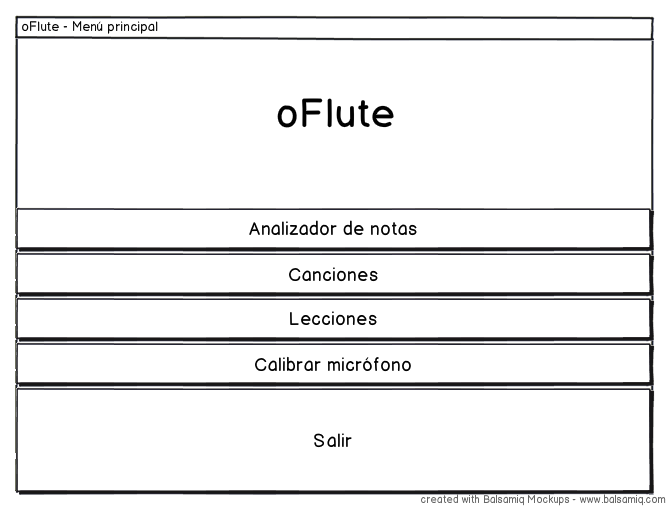
\includegraphics[width=0.6\textwidth]{desarrollo/mockup_menu_principal}
  \caption{Maqueta del menú principal}
\end{figure}

\pagebreak

Las opciones que se incluirán son:
\begin{itemize}
\item \textbf{Analizador de notas}: comprobar las notas que tocamos sobre un
  pentagrama.
\item \textbf{Canciones}: sección principal del juego, en el que aparecerán las
  canciones a tocar.
\item \textbf{Lecciones}: sección de lecciones de aprendizaje.
\item \textbf{Calibrar micrófono}, para ajustarse al nivel de ruido ambiental.
\item \textbf{Salir} al sistema operativo.
\end{itemize}

La siguiente pantalla a modelar será el \textbf{analizador de
  notas}. Simplemente mostrará el logotipo del videojuego a un lado, y un
pentagrama al otro, que se actualizará con la nota detectada por el
micrófono. También contendrá un botón \textit{volver} para ir al menú principal.

\begin{figure}[h!]
  \centering
  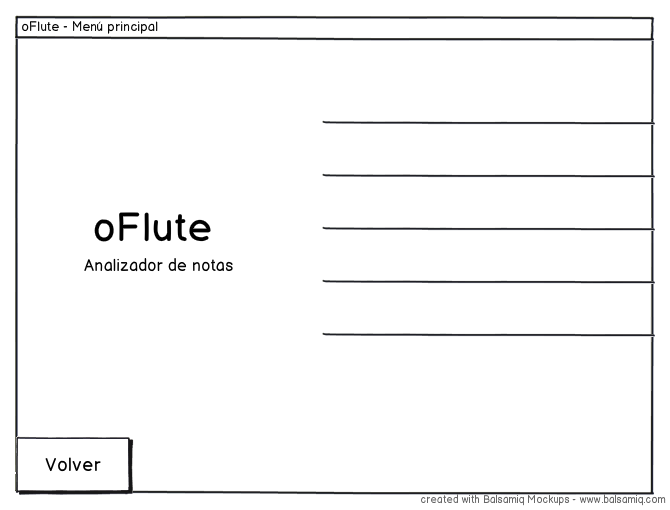
\includegraphics[width=0.6\textwidth]{desarrollo/mockup_analizador}
  \caption{Maqueta de la sección \textit{analizador de notas}}
\end{figure}

La segunda sección a la que se podrá ir desde el menú principal será la de
\textbf{canciones}. Inicialmente, la primera pantalla será la de
\textbf{selección de canción}, que contendrá el logotipo del juego, un botón
para volver al menú principal, y un menú dinámico de canciones que nos permitirá
elegir el tema a interpretar.

\begin{figure}[h!]
  \centering
  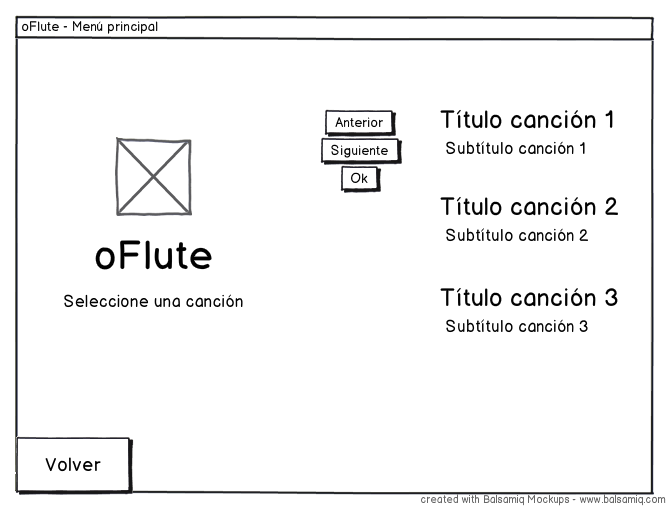
\includegraphics[width=0.6\textwidth]{desarrollo/mockup_seleccionar_cancion}
  \caption{Maqueta del menú de selección de canción}
\end{figure}

Una vez seleccionada la canción, pasaremos a la zona de \textbf{interpretación
  de canción}. Contendrá un pentagrama que ocupará todo el ancho de la pantalla,
con una línea que indicará la zona donde empezar a tocar las notas que
aparezcan. Además, en la parte superior habrá un indicador con la puntuación
obtenida y, abajo, una barra de progreso que nos indicará cuánto queda de
canción.

\begin{figure}[h!]
  \centering
  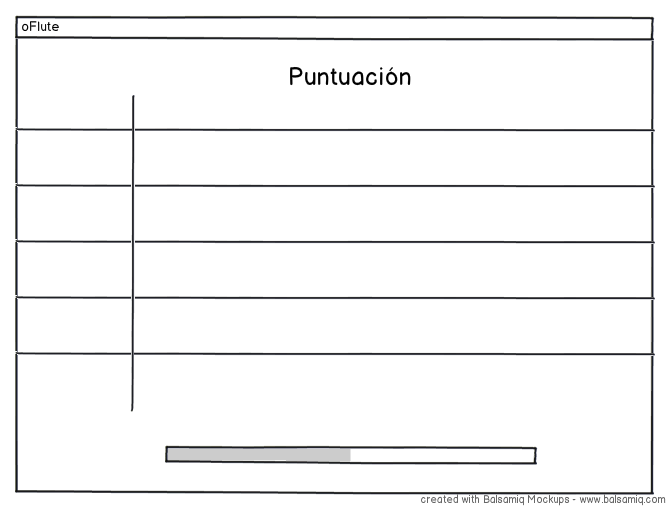
\includegraphics[width=0.6\textwidth]{desarrollo/mockup_reproducir_cancion}
  \caption{Maqueta de la pantalla de interpretación de canción}
\end{figure}

\pagebreak

Al completar la interpretación de la canción, aparecerá la \textbf{sección de
  resultados}. Contendrá el logotipo del juego, el título y subtítulo de la
canción, y un cuadro con información sobre nuestra interpretación, representada
en forma de porcentaje de aciertos. Además, en la zona inferior aparecerá un
mensaje de ánimo dependiendo del resultado obtenido.

\begin{figure}[h!]
  \centering
  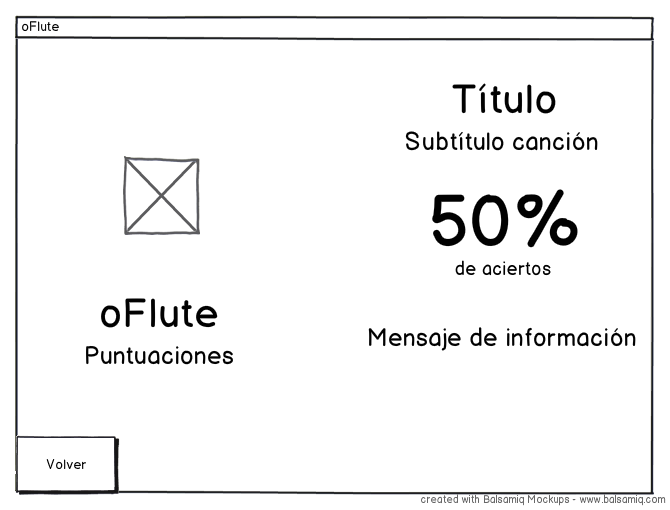
\includegraphics[width=0.6\textwidth]{desarrollo/mockup_puntuaciones}
  \caption{Maqueta de la pantalla de puntuaciones}
\end{figure}

La pantalla de \textbf{selección de lecciones}, a la que se llega desde el menú
principal, contendrá el título, una imagen decorativa, y varios botones para
navegar entre las lecciones cargadas en el sistema. Se mostrará el título y la
descripción de cada lección, así como un botón para comenzar.

\begin{figure}[h!]
  \centering
  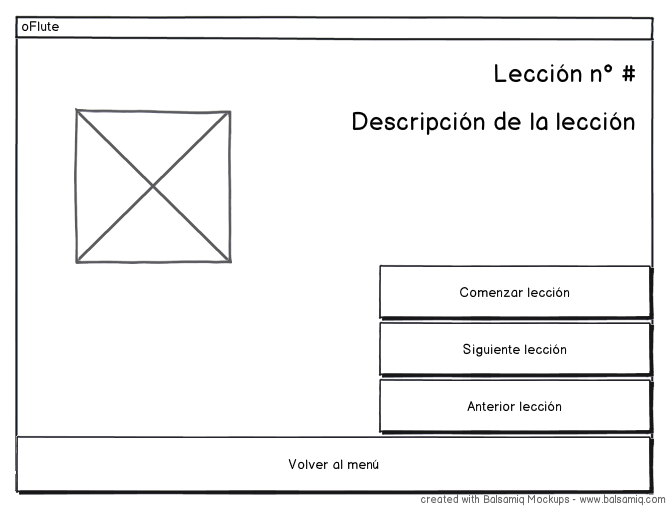
\includegraphics[width=0.6\textwidth]{desarrollo/mockup_seleccionar_leccion}
  \caption{Maqueta del menú de selección de lecciones}
\end{figure}

Una vez elegida una lección, pasaremos a la pantalla de reproducción de
lecciones. Dada la naturaleza \textbf{dinámica} de esta sección, cada lección
podrá tener una apariencia y elementos distintos. El único elemento común entre
todas las lecciones será el botón de \textbf{volver al menú}.

\subsection{Requisitos funcionales}

\textbf{oFlute} se basa en los siguientes requisitos funcionales:
\begin{itemize}
\item Poder terminar la aplicación pulsando el botón de cierre en cualquier
  instante.
\item Comprobar la correcta interpretación de notas individuales mediante el
  analizador de notas.
\item Calibrar el micrófono de forma que el sistema se pueda adaptar al ruido
  ambiental del entorno.
\item Navegar por toda la aplicación de forma sencilla utilizando solo el ratón.
\item Elegir entre varias canciones a interpretar, cada una con su título y
  subtítulo informativos.
\item Interpretar las canciones mediante el uso de la flauta, siguiendo el
  pentagrama en pantalla.
\item Elegir entre bastantes lecciones informativas, poder ejecutarlas y
  seguirlas.
\item Capacidad de añadir nuevas lecciones y canciones de forma sencilla.
\end{itemize}

\subsection{Requisitos de rendimiento}

La aplicación \textbf{oFlute} precisa de unos requisitos bastante básicos,
que en su mayor parte se reducen a cuatro puntos principales:
\begin{itemize}
\item Posesión de una tarjeta de sonido o subsistema de audio similar con un
  micrófono, para poder captar el sonido de la flauta.
\item Pantalla con una resolución de, al menos, 800 por 600 píxeles.
\item Sistema gráfico compatible con OpenGL.
\item Dispositivo apuntador, como un ratón.
\end{itemize}

La práctica totalidad de los ordenadores personales de la actualidad cumplen los
citados requisitos.

\subsection{Requisitos de diseño}
\marginpar{¿?¿?¿?}

\subsection{Requisitos del sistema software}
El sistema de software deberá cumpliar los requisitos siguientes:
\begin{itemize}
\item Deberá funcionar en cualquier sistema \textbf{GNU/Linux} con los
  requisitos anteriormente indicados.
\item Deberá limitarse el número de dependencias, así como facilitar al máximo
  la instalación de las que resultasen imprescindibles.
\item El uso del teclado quedará en segundo plano, haciendo posible utilizar la
  aplicación completamente con el ratón.
\item Al tratarse de un público objetivo juvenil, la aplicación deberá ser
  dinámica, intuitiva y fácil de usar, y la apariencia debe ser agradable.
\item Se evitará el uso de constantes y recursos dentro del código de la
  aplicación, utilizando como alternativa ficheros para representar las
  lecciones y las canciones.
\end{itemize}

\section{Modelo de casos de uso}

A la hora de modelar los casos de uso del sistema, hemos optado por utilizar
notación \textit{UML}, siguiendo los siguientes pasos:
\begin{itemize}
\item Identificación de los usuarios del sistema y sus roles.
\item Para cada rol, determinar las formas de interactuar con el sistema.
\item Creación de casos de uso para los objetivos que debe cumplir la aplicación.
\item Modularización de los casos de usos mediante la implementación de
  relaciones de inclusión o extensión.
\end{itemize}

\subsection{Diagrama de casos de uso}

\begin{figure}[h!]
  \centering
  \includegraphics[width=0.81\textwidth]{desarrollo/diagrama_de_casos_de_uso}
  \caption{Diagrama de casos de uso}
\end{figure}


\subsection{Descripción de los casos de uso}

\subsubsection{Caso de uso: inicio del juego}
\begin{description}
\item [Descripción] Se muestran los créditos del juego, la pantalla de
  presentación, y finalmente el menú principal, desde donde se accederá al
  resto de secciones del juego.
\item [Actores] \jugador.
\item [Precondiciones] Ninguna.
\item [Postcondiciones] Ninguna.
\item [Escenario principal] $\quad$
  \begin{enumerate}
  \item El \jugador\ inicia la aplicación.
  \item El \sistema\ inicializa el subsistema gráfico.
  \item El \sistema\ muestra la pantalla de créditos y la pantalla de
    presentación de la aplicación.
  \item El \sistema\ muestra el menú principal en la pantalla.
  \item El \jugador\ selecciona la opción \textit{Canciones}.
  \item El \sistema\ accede a la pantalla de \textit{Selección de canción}.
  \end{enumerate}
\item[Extensiones --- flujo alternativo] $\quad$
  \begin{description}
  \item [*a] El \jugador\ cierra la ventana.
    \begin{enumerate}
    \item El \sistema\ libera los recursos y sale de la aplicación.
    \end{enumerate}
  \item [4a] El \jugador\ selecciona la opción \textit{Analizador de Notas}.
    \begin{enumerate}
    \item El \sistema\ accede a la pantalla del analizador de notas.
    \end{enumerate}

  \item[4b] El \jugador\ selecciona la opción \textit{Lecciones}.
    \begin{enumerate}
    \item El \sistema\ accede a la pantalla de \textit{Selección de lecciones}.
    \end{enumerate}
  \item[4c] El \jugador\ selecciona la opción \textit{Calibrar micrófono}.
    \begin{enumerate}
    \item El \sistema\ accede a la pantalla de calibración de micrófono.
    \end{enumerate}
  \item [4d] El \jugador\ selecciona la opción Salir.
    \begin{enumerate}
    \item El \sistema\ libera los recursos y sale de la aplicación.\\
    \end{enumerate}
  \end{description}  
\end{description}


\subsubsection{Caso de uso: selección de canción}

\begin{description}
\item [Descripción] Al \jugador\ se le muestra una lista de las canciones
  detectadas, y éste debe elegir entre ellas la que desea interpretar, o volver
  al menú princial.
\item [Actores] \jugador.
\item [Precondiciones] Ninguna.
\item [Postcondiciones] Una canción queda seleccionada.
\item [Escenario principal] $\quad$
  \begin{enumerate}
  \item El \jugador\ accede, desde el menú principal, al panel de selección de canciones.
  \item El \sistema\ busca las canciones dadas de alta en el juego y muestra un menú con las mismas.
  \item El \jugador\ navega entre las canciones listadas y selecciona una de ellas, pulsando finalmente el botón \textit{Ok}.
  \item El \sistema\ carga la canción y pasa a la pantalla de interpretación de canciones.
  \end{enumerate}
\item[Extensiones --- flujo alternativo] $\quad$
  \begin{description}
  \item [*a] El \jugador\ cierra la ventana.
    \begin{enumerate}
    \item El \sistema\ libera los recursos y sale de la aplicación.
    \end{enumerate}
  \item [3a] El \jugador\ selecciona la opción \textit{Volver}.
    \begin{enumerate}
    \item El \sistema\ muestra la animación de cierre y vuelve al menú principal.
    \end{enumerate}
  \end{description}  
\end{description}


\subsubsection{Caso de uso: interpretación de canción}

\begin{description}
\item [Descripción] Tras haber elegido la canción a interpretar, se muestra una
  partitura con las notas que el \jugador\ deberá tocar para conseguir la puntuación deseada.
\item [Actores] \jugador.
\item [Precondiciones] Se ha elegido una canción.
\item [Postcondiciones] Se completa la interpretación de la canción, obteniendo una calificación
\item [Escenario principal] $\quad$
  \begin{enumerate}
  \item El \sistema\ carga la canción, leyendo las notas, y muestra en pantalla,
    mediante animaciones, el marcador de puntos y el pentagrama.
  \item El \sistema\ comienza a mostrar notas en el pentagrama, que van
    deslizándose hacia el lado izquierdo, en el que se encuentra la aguja de
    reproducción, e inicia el análisis del sonido.
  \item El \jugador\, al llegar la nota a la aguja de reproducción, toca la
    flauta con la altura y la duración correcta, de forma que el micrófono sea
    capaz de captar el sonido.
  \item El \sistema\ analiza el sonido que captura el micrófono y detecta la nota que toca el usuario.
  \item El \sistema\ determina que la nota es la correcta y suma los puntos correspondientes.
  \item Mientras existan más notas, se vuelve al punto 2.
  \item El \sistema\ determina que no hay más notas que mostrar, e inicia las
    animaciones para ocultar los elementos en pantalla.
  \item El \sistema\ pasa a la sección de \textit{Resultados de la interpretación}.
  \end{enumerate}
\item[Extensiones --- flujo alternativo] $\quad$
  \begin{description}

  \item [*a] El \jugador\ cierra la ventana.
    \begin{enumerate}
    \item El \sistema\ libera los recursos y sale de la aplicación.
    \end{enumerate}

  \item[*b] El \jugador\ pulsa la tecla \texttt{escape}.
    \begin{enumerate}
    \item El \sistema\ vuelve a la pantalla de \textit{selección de canción}.
    \end{enumerate}

  \item [3a] El \jugador\ toca el instrumento con intensidad insuficiente o nula
    y el sonido no llega al sistema.
    \begin{enumerate}
    \item El \sistema\ representa esta inconsistencia como un silencio.
    \end{enumerate}

  \item [4a] El \sistema\ no es capaz de determinar fehacientemente la nota que
    toca el usuario.
    \begin{enumerate}
    \item El \sistema\ representa esta inconsistencia como un silencio.
    \end{enumerate}

  \item[5a] El \sistema\ determina que la nota tocada por el usuario no es la
    que corresponde a la partitura.
    \begin{enumerate}
    \item El \sistema\ ignora esta situación y no suma los puntos al marcador.
    \end{enumerate}

  \end{description}  
\end{description}

\subsubsection{Caso de uso: resultados de la interpretación}

\begin{description}
\item [Descripción] Después de interpretar las notas de la partitura, se
  muestran los datos obtenidos del análisis de las notas tocadas por el \jugador.
\item [Actores] \jugador.
\item [Precondiciones] Se ha elegido e interpretado una canción.
\item [Postcondiciones] Se completa la partida actual.
\item [Escenario principal] $\quad$
  \begin{enumerate}
  \item El \sistema\ compara la puntuación conseguida con la máxima puntuación
    obtenible, y genera un porcentaje de aciertos.
  \item El \sistema\ muestra, mediante animaciones, un mensaje con información
    sobre la canción y sobre la interpretación del \jugador\, representada
    mediante un porcentaje de aciertos.
  \item El \sistema\ muestra un mensaje variable en función del número de
    aciertos conseguido.
  \item El \jugador\ revisa su puntuación y pulsa el botón \textit{volver} para
    ir de vuelta al menú de \textit{selección de canción}.
  \end{enumerate}
\item[Extensiones --- flujo alternativo] $\quad$
  \begin{description}

  \item [*a] El \jugador\ cierra la ventana.
    \begin{enumerate}
    \item El \sistema\ libera los recursos y sale de la aplicación.
    \end{enumerate}

  \item[4a] El \jugador\ pulsa la tecla \texttt{escape}.
    \begin{enumerate}
    \item El \sistema\ vuelve a la pantalla de \textit{selección de canción}.
    \end{enumerate}

  \end{description}  
\end{description}


\subsubsection{Caso de uso: analizador de notas}

\begin{description}
\item [Descripción] El \jugador\ elige la opción \textit{analizador de notas} en
  el menú principal y es llevado a esta sección, en la que el sistema
  representará gráficamente la nota que esté tocando con la flauta en cada
  instante, sin otra interacción
\item [Actores] \jugador.
\item [Precondiciones] Ninguna.
\item [Postcondiciones] Ninguna
\item [Escenario principal] $\quad$
  \begin{enumerate}
  \item El \jugador\ accede, desde el menú principal, al panel del analizador de notas.
  \item El \sistema\ muestra, mediante animaciones, la pantalla de la sección,
    representada mediante una fracción de partitura en la que se representará la
    nota que esté tocando el \jugador\ en cada momento.
  \item El \sistema\ inicia el análisis del sonido.
  \item El \jugador\ toca la nota que desee con su flauta, de forma que el
    micrófono sea capaz de captar el sonido.
  \item El \sistema\ analiza el sonido que captura el micrófono y detecta la
    nota que toca el usuario.
  \item El \sistema\ muestra en pantalla la nota, sobre la partitura,
    correspondiente a lo que ha tocado el usuario.
  \item Se repite el flujo desde el punto 4, mientras el \jugador\ no pulse en
    el botón volver.
  \item El \jugador\ pulsa en el botón \textit{volver}.
  \item El \sistema\ inicia las animaciones para ocultar los elementos en pantalla.
  \item El \sistema\ vuelve al menú principal.
  \end{enumerate}
\item[Extensiones --- flujo alternativo] $\quad$
  \begin{description}

  \item [*a] El \jugador\ cierra la ventana.
    \begin{enumerate}
    \item El \sistema\ libera los recursos y sale de la aplicación.
    \end{enumerate}

  \item[*b] El \jugador\ pulsa la tecla \texttt{escape}.
    \begin{enumerate}
    \item El \sistema\ vuelve al menú principal.
    \end{enumerate}

  \item [4a] El \jugador\ toca el instrumento con intensidad insuficiente o nula
    y el sonido no llega al sistema.
    \begin{enumerate}
    \item El \sistema\ representa esta inconsistencia como un silencio.
    \end{enumerate}

  \item [5a] El \sistema\ no es capaz de determinar fehacientemente la nota que
    toca el usuario.
    \begin{enumerate}
    \item El \sistema\ representa esta inconsistencia como un silencio.
    \end{enumerate}
  \end{description}  
\end{description}

\subsubsection{Caso de uso: calibración de micrófono}
\begin{description}
\item [Descripción] El \jugador\ elige la opción \textit{calibrar micrófono} en
  el menú principal y es llevado a esta sección, en la que el \sistema\ calibrará
  el micrófono de forma que sea posible aislar el sonido de la flauta del ruido
  ambiental.
\item [Actores] \jugador.
\item [Precondiciones] Ninguna.
\item [Postcondiciones] El \sistema\ obtiene un valor umbral con el que
  discernir entre el sonido del instrumento y el ruido ambiente.
\item [Escenario principal] $\quad$
  \begin{enumerate}
  \item El \jugador\ accede, desde el menú principal, al panel de calibración del micrófono.
  \item El \sistema\ muestra la sección, indicando con un mensaje que el usuario
    debe pulsar la tecla \texttt{escape} para iniciar la calibración.
  \item El \jugador\ pulsa la tecla \texttt{escape} y se mantiene en silencio.
  \item El \sistema\ inicia el análisis del sonido, guardando durante dos
    segundos los valores de ruido que lee del micrófono.
  \item El \sistema\ calcula, a partir de los valores leídos, el umbral de
    ruido, y muestra un mensaje informando del final del proceso.
  \item El \jugador\ pulsa la tecla \texttt{escape} y el \sistema\ vuelve al
    menú principal.
  \end{enumerate}
\item[Extensiones --- flujo alternativo] $\quad$
  \begin{description}

  \item [*a] El \jugador\ cierra la ventana.
    \begin{enumerate}
    \item El \sistema\ libera los recursos y sale de la aplicación.
    \end{enumerate}

  \item[*b] El \jugador\ pulsa la tecla \texttt{escape}.
    \begin{enumerate}
    \item El \sistema\ cancela la calibración y vuelve al menú principal.
    \end{enumerate}

  \item [5a] El \sistema\ encuentra valores inválidos al leer el ruido
    ambiental.
    \begin{enumerate}
    \item El \sistema\ informa al usuario del fallo del proceso de calibración.
    \item El \jugador\ pulsa la tecla \texttt{escape} y el \sistema\ vuelve al
      menú principal.
    \end{enumerate}
  \end{description}  
\end{description}

\subsubsection{Caso de uso: selección de lecciones}
\begin{description}
\item [Descripción] El \jugador\ elige la opción \textit{lecciones} en el menú
  principal y es llevado a esta sección, en la que el \sistema\ mostrará una
  lista de lecciones cargadas, entre las que el usuario deberá elegir.
\item [Actores] \jugador.
\item [Precondiciones] Ninguna.
\item [Postcondiciones] Se ha elegido una lección
\item [Escenario principal] $\quad$
  \begin{enumerate}
  \item El \jugador\ accede, desde el menú principal, al panel de selección de lecciones.
  \item El \sistema\ carga la lista de secciones y muestra, mediante
    animaciones, el panel, preseleccionando por defecto la primera lección.
  \item El \jugador\ utiliza los botones de la sección para elegir una de las
    lecciones, y activarla pulsando \textit{comenzar lección}.
  \item El \sistema\ oculta de forma animada el panel de selección de lecciones.
  \item El \sistema\ lee el fichero \texttt{xml} asociado a la lección indicada,
    cargando los elementos que la componen y las animaciones que se ejecutarán.
  \item El \sistema\ ejecuta las animaciones correspondientes a los elementos
    multimedia de la lección.
  \end{enumerate}
\item[Extensiones --- flujo alternativo] $\quad$
  \begin{description}

  \item [*a] El \jugador\ cierra la ventana.
    \begin{enumerate}
    \item El \sistema\ libera los recursos y sale de la aplicación.
    \end{enumerate}

  \item[2a] El \sistema\ detecta que una de las lecciones leídas no está
    correctamente construída.
    \begin{enumerate}
    \item El \sistema\ informa del error en el \textit{log} del programa y omite
      la carga de esa lección.
    \end{enumerate}

  \item[3a] El \jugador\ pulsa la tecla \texttt{escape}.
    \begin{enumerate}
    \item El \sistema\ vuelve al menú principal.
    \end{enumerate}

  \item[6a] El \jugador\ pulsa la tecla \texttt{escape}.
    \begin{enumerate}
    \item El \sistema\ vuelve al menú de selección de lecciones.
    \end{enumerate}

  \end{description}  
\end{description}

\section{Modelo conceptual de datos}

El modelo conceptual de datos representa, de forma esquemática, las clases que
modelan el sistema y las relaciones que existen entre ellas, además de una
pequeña introducción a su utilidad. 


%\chapter{Resumen}
%\documentclass[a4paper,11pt]{article}

\usepackage{estiloBase}
\usepackage{colores}
\usepackage{bera}
\usepackage{comandos}

\addto\captionsspanish{
\renewcommand\bibname{Bibliografía y referencias}
}

\def \titulo{oFlute: reconocimiento de señales aplicado al aprendizaje de la flauta dulce}
\def \autor{Alumno: José Tomás Tocino García\\Tutores: Manuel Palomo Duarte, Antonio García Domínguez}
\def \fecha{Agosto de 2010}

%\margenes

% Directorio de imágenes
%\graphicspath{{../img/}}

\begin{document}
\portada

\abstract{\textbf{oFlute} se modela como una herramienta lúdico-educativa para
  alumnos que comiencen a aprender a usar la flauta dulce, proporcionando un
  entorno atractivo y ameno para el estudiante. Éstos tendrán la posibilidad de
  comprobar sus conocimientos sobre el uso de la flauta de forma totalmente
  práctica, gracias a un motor de análisis del sonido capaz de detectar las
  notas que emite el jugador con la flauta, capturadas por un micrófono,
  mediante el que la aplicación valorará la pericia del estudiante con la
  flauta.

  Además, los jugadores podrán recorrer una serie de pequeñas lecciones sobre
  música en general, y el uso de la flauta dulce en particular. Estas lecciones
  son totalmente ampliables, dando al usuario la posibilidad de crear las suyas
  propias. Liberado bajo una licencia open-source y desarrollado utilizando
  software libre, oFlute está abierto a cualquier clase de ampliación o aporte
  de terceros, facilitando para ello el código fuente y sus recursos de manera
  libre. }

\vspace{0.5cm}

\begin{center}
{\footnotesize Este documento se halla bajo la licencia FDL de GNU (Free Documentation
  License)\\ \url{http://www.gnu.org/licenses/fdl.html} }   
\end{center}



\tableofcontents

\lstset{style=C++}

%\setlength{\parskip}{0.3cm plus 3mm}
\setlength{\parindent}{0.3cm}
\setlength{\parskip}{1.2ex plus 0.4ex minus 0.2ex}

\section{Introducción}

\subsection{Contexto y motivación}
Las nuevas tecnologías van filtrándose gradualmente en los centros
educativos, y las técnicas de enseñanza se están adaptando a las
opciones que ofrecen. El reparto de ordenadores portátiles a los
alumnos andaluces de 5º y 6º de primaria, dentro del marco de la
Escuela TIC 2.0, es buena muestra de ello. 

Por otro lado, las nuevas generaciones están en plena simbiosis con las
tecnologías de la información, cada vez más acostumbradas al empleo de
dispositivos electrónicos interactivos, y su uso ya les es prácticamente
instintivo. Por tanto, es beneficioso buscar nuevos métodos educativos que hagan
uso de las nuevas tecnologías.

En la búsqueda de materias educativas en las que aplicar el uso de las nuevas
tecnologías, la música, parte fundamental del programa curricular en la
educación primaria, ofrece una gran variedad de aspectos que podrían
desarrollarse utilizando tecnologías de la información. Es ahí donde este
proyecto hace su aportación, en la flauta dulce, un instrumento económico y
fácil de aprender que se usa tradicionalmente en la educación musical
obligatoria en España.

\textbf{oFlute} se modela como una herramienta lúdico-educativa para alumnos que
comiencen a aprender a usar la flauta dulce, proporcionando un entorno atractivo
y ameno para el estudiante. Éstos tendrán la posibilidad de comprobar sus
conocimientos sobre el uso de la flauta de forma totalmente práctica, gracias a
un motor de análisis del sonido capaz de detectar las notas que emite el jugador
con la flauta, capturadas por un micrófono, mediante el que la aplicación
valorará la pericia del estudiante con la flauta.

\subsection{Objetivos}
Los principales objetivos a alcanzar con \textbf{oFlute} son los siguientes:

\begin{itemize}
\item Crear un \textbf{módulo de análisis del sonido} en el dominio de la
  frecuencia para poder identificar las notas emitidas por una flauta dulce y
  capturadas mediante un micrófono en tiempo real.
\item Crear una \textbf{aplicación} de usuario que identifique y muestre en
  pantalla las notas que toca el usuario con la flauta dulce en cada momento.
\item Reutilizar el módulo de análisis en un juego en el que el usuario debe
  \textbf{ interpretar una canción} tocando correctamente las notas que aparecen
  en pantalla sobre un pentagrama.
\item Incluir un \textbf{sistema de lecciones} multimedia individuales que
  sirvan al alumno de referencia y fuente de aprendizaje.
\item Potenciar el uso de \textbf{interfaces de usuario amigables}, con un
  sistema avanzado de animaciones que proporcione un aspecto fluido y evite
  saltos bruscos entre secciones.
\item Obtener una \textbf{base teórica} sobre cómo se representa y caracteriza
  digitalmente el sonido.
\item Conocer las \textbf{bases del DSP}, y su uso en aplicaciones de
  reconocimiento básico de sonidos, tales como sintonizadores y afinadores de
  instrumentos.
\item Adquirir soltura en la \textbf{programación de audio} bajo sistemas
  GNU/Linux.
\item Utilizar un enfoque de análisis, diseño y codificación \textbf{orientado a
    objetos}, de una forma lo más clara y modular posible, para permitir
  ampliaciones y modificaciones sobre la aplicación por terceras personas.
\item Hacer uso de herramientas básicas en el desarrollo de software, como son
  los Sistemas de Control de Versiones para llevar un control realista del
  desarrollo del software, así como hacer de las veces de sistema de copias de
  seguridad.

\end{itemize}

\section{Planificación}
El proyecto se ha desarrollado siguiendo un calendario basado en fases,
utilizando un modelo de desarrollo iterativo incremental.

\subsection{Primera iteración: conocimientos preliminares}
En esta etapa se adquirieron los fundamentos teóricos para poder afrontar el
desarrollo con todas las garantías. Se llevaron a cabo labores de documentación
y aprendizaje autodidacta con las que se asentaron los conocimientos necesarios.

\subsection{Segunda iteración: analizador básico}
La segunda iteración se basó en el diseño de un analizador de notas básico, que
sería el corazón del programa. Del éxito del desarrollo temprano del módulo que
se encargaría del análisis de sonidos dependería la viabilidad completa del
proyecto.

\subsection{Tercera iteración: interfaz gráfica de usuario}
En esta tercera iteración se propusieron numerosos diseños para la interfaz
gráfica de usuario y se comenzó el desarrollo de los elementos de la interfaz,
haciendo énfasis en conseguir un aspecto dinámico y jovial.

\subsection{Cuarta iteración: motor de lecciones}
En esta iteración se llevó a cabo el motor de lecciones, que presenta una serie
de unidades didácticas en formato multimedia, compuestas de imágenes y
textos. El sistema resultante es muy sencillo de ampliar y utilizar.

\subsection{Quinta iteración: motor de canciones}
Durante la quinta iteración se elaboró el sistema de canciones, encargado de
listar y cargar las diferentes canciones, y puntuar al usuario según cómo
interprete, mediante la flauta, las canciones que aparece en pantalla.. Es la
parte de la aplicación con mayor interactividad.

\subsection{Diagrama de Gantt}
Se ha diseñado un diagrama de Gantt para reflejar la distribución de las tareas
a lo largo del tiempo (figura~\ref{fig:gantt} en la página~\pageref{fig:gantt}).

\section{Descripción general}
\textbf{oFlute} se modela como una herramienta lúdico-educativa para alumnos que
comiencen a aprender a usar la flauta dulce, proporcionando un entorno atractivo
y ameno para el estudiante. Éstos tendrán la posibilidad de comprobar sus
conocimientos sobre el uso de la flauta de forma totalmente práctica, gracias a
un motor de análisis del sonido capaz de detectar las notas que emite el jugador
con la flauta, capturadas por un micrófono, mediante el que la aplicación
valorará la pericia del estudiante con la flauta.

Además, los jugadores podrán recorrer una serie de pequeñas lecciones sobre
música en general, y el uso de la flauta dulce en particular. Estas lecciones
son totalmente ampliables, dando al usuario la posibilidad de crear las suyas
propias.

La aplicación cuenta con varias funcionalidades bien diferenciadas. A
continuación se detallan cada una de ellas.

\begin{figure}[htp!]
  \vspace{1cm}
  \centering
  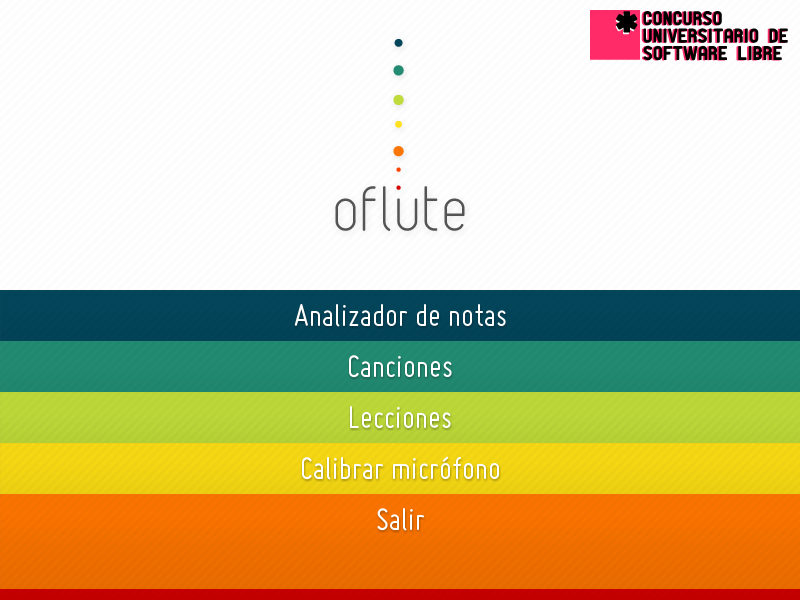
\includegraphics[width=0.8\textwidth]{imagen_menuPrincipal}
  \caption{Pantalla del menú principal}
\end{figure}

\pagebreak

\begin{figure}[htp!]
  \centering
  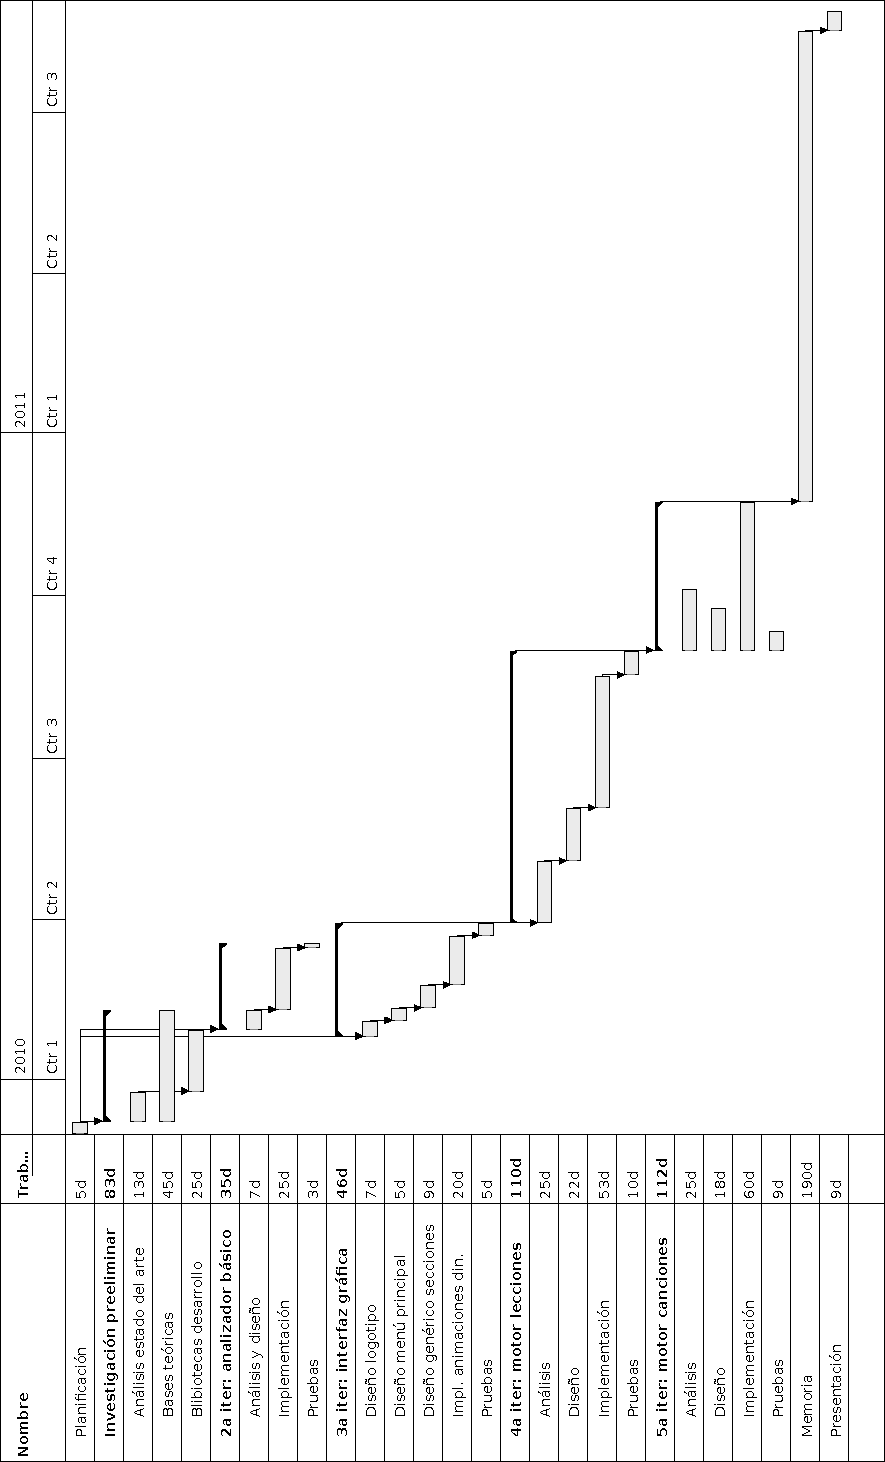
\includegraphics[width=0.95\textwidth]{imagen_diagrama_gantt}
  \caption{Diagrama Gantt de iteraciones}
  \label{fig:gantt}
\end{figure}

\pagebreak

\subsection{Análisis de notas}
Permite a los usuarios comprobar, de manera individual y pausada, que la
interpretación de cada una de las notas en la flauta es correcta. Para ello, se
presenta un pequeño analizador que responderá al sonido emitido por el usuario
con la flauta mostrando la nota tocada en pantalla.

\begin{figure}[h!]
  \centering
  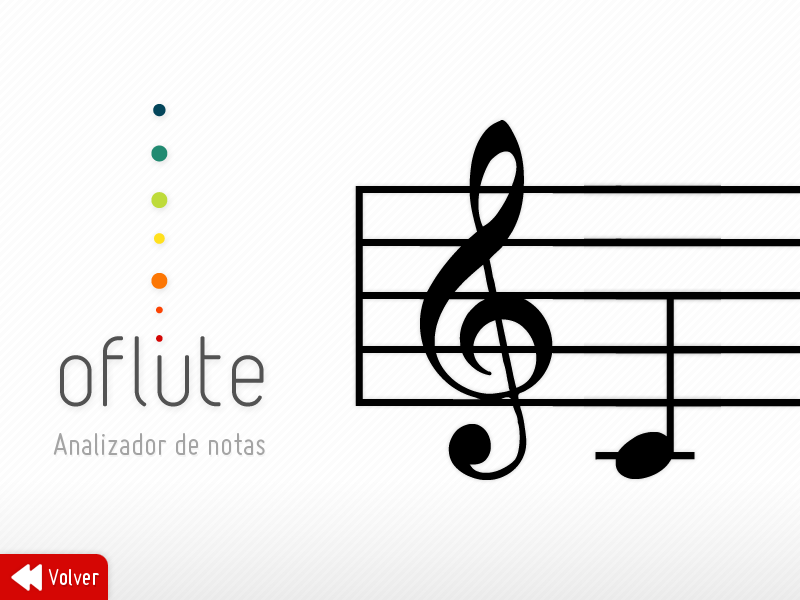
\includegraphics[width=0.8\textwidth]{imagen_seccionAnalizador}
  \caption{Pantalla del analizador de notas}
\end{figure}

\subsection{Motor de canciones}
Mediante este sistema, el usuario tendrá la oportunidad de interpretar canciones
completas a la vez que el computador analiza la eficacia del jugador,
otorgándole una puntuación en tiempo real. Además, el motor de canciones es
fácilmente expansible mediante ficheros de definición de canciones.

\subsection{Motor de lecciones}
Este sistema ofrece al usuario una serie de lecciones multimedia, con las que
podrá aprender sobre diferentes aspectos de la música en general y la flauta en
particular. Las lecciones cuentan con imágenes, texto y animaciones, que harán
que el aprendizaje sea entretenido y ameno. También es posible añadir nuevas
lecciones al sistema de forma sencilla.

\begin{figure}[h!]
  \centering
  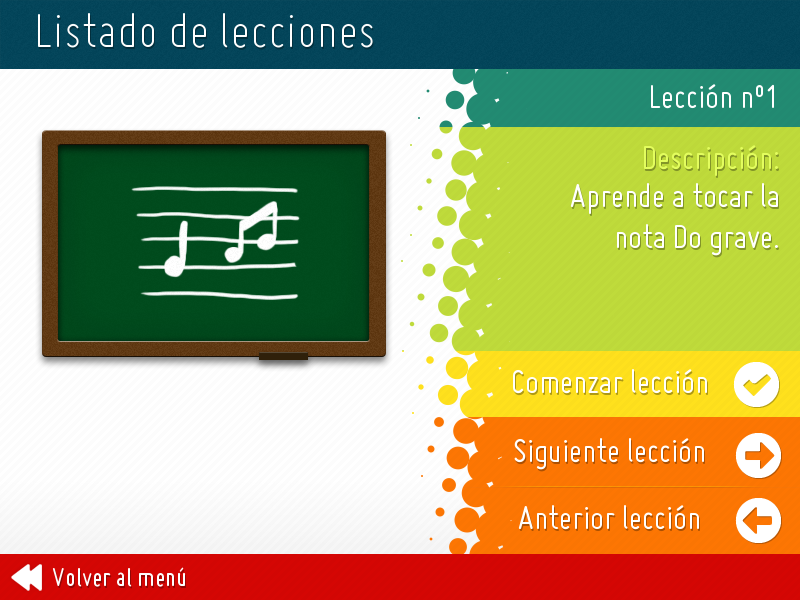
\includegraphics[width=0.8\textwidth]{imagen_seccionLecciones1}
  \caption{Pantalla del menú de selección de lecciones}
\end{figure}

\subsection{Calibración del micrófono}
\textbf{oFlute} ofrece la posibilidad de calibrar el micrófono, de forma que el
sistema se adapte al ruido ambiental y el análisis del sonido capturado sea lo
más exacto posible

\section{Implementación}
Durante el desarrollo del proyecto surgieron numerosas cuestiones y decisiones
de implementación. A continuación se presenta una selección de las que más
interés han generado. En la memoria del proyecto se desarrollan en mayor
extensión.

\subsection{Implementación del analizador básico}
La creación del analizador básico de notas era crucial para el buen transcurso
del resto del proyecto, por lo que fue uno de los objetivos que antes se
abordaron. El desarrollo se dividió en dos partes. Por un lado, había que
iniciar la captura de audio, lanzando el subsistema de sonido y empezando a
capturar datos. Por otro lado, se tenía que hacer el análisis de los datos
leídos para determinar qué nota se estaba tocando.

La gestión del subsistema de audio se hizo mediante la \textit{Simple API} de
PulseAudio, la biblioteca de audio que se empleó en oFlute. Se utilizó para la
configuración y creación de un flujo de audio de entrada que permitiera captar,
muestrear y samplear el sonido del micrófono, ofreciéndolo en forma de datos en
punto flotante en un búffer.

El siguiente paso fue el análisis del audio capturado. Para ello, utilizamos la
Transformada Rápida de Fourier mediante su implementación en la biblioteca
KissFFT. De forma iterativa, se iba analizando el búffer de sonido cada vez que
éste se llenaba, dando lugar a una aproximación de la frecuencia fundamental
capturada y, por ende, la nota que se estaba interpretando con la flauta.

Una vez implementado y probado el sistema, se dió por bueno el analizador y se
siguió construyendo el resto de la aplicación

\subsection{Carga y uso de fuentes TrueType en Gosu}
La biblioteca principal utilizada en la implementación del proyecto es Gosu, una
librería de desarrollo de videojuegos 2D, multi-plataforma y con numerosas
características. Desafortunadamente, no era posible utilizar fuentes TrueType
cuando se utilizaba la biblioteca en GNU/Linux.

Utilizando los conocimientos de otra popular biblioteca, SDL, se consiguió
implementar un sistema para cargar y usar fuentes TrueType en Gosu de forma
eficiente. Esta implementación finalmente acabó formando parte oficial de la
biblioteca Gosu.

\subsection{Animaciones dinámicas}
Una de las decisiones iniciales de diseño fue la de hacer la interfaz gráfica de
usuario lo más atractiva posible, intentando utilizar gráficos amigables y, en
la medida de lo posible, animaciones y efectos dinámicos.

Con esto, se tornaba necesario crear un sistema de animaciones lo más versátil
posible, de forma que dotar a los elementos de la interfaz de movimiento fuera
un proceso sencillo. 

Para satisfacer este objetivo se ideó una serie de clases de animación que
permiten animar las propiedades de los objetos de manera muy sencilla. Mediante
el uso de las ecuaciones de animación de Robert Penner, el sistema creado cuenta
con un gran número de opciones y diferentes formas de movimiento, según el tipo
de función utilizada para calcular los valores: cuadrático, cúbico, etcétera.

Gracias a este sistema, la interfaz de usuario de oFlute cuenta con un gran
dinamismo y vistosidad.

\subsection{Gestión de estados}
La gestión de estados es uno de los retos principales a la hora de desarrollar
un videojuego. Es necesario contar un sistema de gestión de estados robusto, que
permita pasar de un estado a otro de forma sencilla, sin errores, y manteniendo
información entre transiciones si fuera necesario.

En el caso de oFlute, se creó un gestor de estados que permitió modularizar
fácilmente el programa, haciendo una clara división entre secciones y
facilitando la transición entre ellas. Además, mediante pruebas exhaustivas y el
uso de herramientas de depuración, el gestor está implementado de forma que la
carga y descarga de estados sea limpia y sin errores, evitando fugas de memoria.

\subsection{Internacionalización}
Durante el desarrolllo del proyecto surgió la necesidad de preparar el proyecto
para su traducción. Inicialmente se optó por utilizar un sistema propio de
traducción, basado en un script en Python y en una pequeña clase que generaba un
diccionario según el idioma elegido. Sin embargo, esta opción resultó
ineficiente y, sobre todo, alejada del resto de soluciones estándar a la hora de
traducción de proyectos. 

Por ello, se decidió investigar sobre las tecnologías de traducción más
utilizadas en el panorama del software libre, y finalmente se optó por
\textbf{GNU Gettext}~\cite{refgettext}. Para afianzar los conocimientos y
facilitar el aprendizaje a otros desarrolladores, se editó un conciso manual
sobre internacionalización de proyectos, presente como apéndice en la memoria del proyecto fin de



\section{Conclusiones y difusión}
Durante el transcurso del desarrollo de oFlute, y sobre todo al término del
mismo, se han obtenido unas conclusiones y unos resultados, tanto de forma
personal como para con la comunidad, que se resumen en esta sección y se tratan
más en profundidad en el capítulo dedicado a tal efecto en la memoria principal.

\subsection{Objetivos}
Al término del desarrollo del proyecto, el proyecto ha completado todos los
objetivos a cumplir, detallados en el planteamiento inicial. En particular:

\begin{itemize}
\item Se llevó a cabo la creación del módulo de análisis de sonido, consiguiendo
  una efectividad en la detección de las notas muy alta.
\item Se hizo uso del módulo en una sección de análisis de notas y en el propio
  juego de interpretación de canciones, con resultados muy satisfactorios y
  funcionamiento correcto.
\item Además, el sistema de lecciones planteado se llevó a cabo correctamente,
  consiguiendo un motor dinámico bastante potente y fácilmente ampliable, con
  opción a añadir nuevas lecciones al sistema.
\item Finalmente, todos los objetivos se llevaron a cabo respetando la premisa
  de mantener una interfaz de usuario amigable y fluida, agradable a la vista y
  sencilla de usar.
\end{itemize}

\subsection{Posibles mejoras}
Hay un gran número de posibles mejoras y extensiones de la funcionalidad de
oFlute, en unos casos descubiertas de forma personal y en otros casos aportadas
por terceras personas. Algunas de las más interesantes son las siguientes:
\begin{itemize}
\item Extensión del sistema de lecciones para permitir lecciones de varios
  pasos, así como integrar las lecciones con el analizador de audio para
  comprobar los conocimientos in-situ.
\item Mejora de la jugabilidad del sistema de canciones, añadiendo bonus y
  puntos extra.
\item Intentar extender el sistema a otros instrumentos o a la voz humana.
\item Portar el videojuego a la plataforma Windows.
\end{itemize}

\subsection{Conclusiones personales}

oFlute ha sido el proyecto más longevo al que me he enfrentado hasta ahora. A
pesar de tener conciencia de la envergadura del mismo desde el principio, el
tiempo para completarlo ha superado todas mis expectativas, sobre todo en lo que
a documentación se refiere. 

Gracias a oFlute he aprendido las técnicas básicas de la programación de audio,
sobre todo en la parte técnica más que teórica. Es esta parte teórica, sobre
todo la de análisis, la que me gustaría reforzar en un futuro, ahora que cuento
con las bases para conseguirlo. Los videojuegos relacionados con el audio
son un nicho aún poco explorado y que puede dar muchas satisfacciones, sobre
todo cuando el producto se orienta a un público joven.

Por otro lado, oFlute también me ha ayudado a aprender a usar bastantes
tecnologías auxiliares, en algunos casos meras herramientas que han facilitado
el trabajo y, en otros casos, elementos que resultaron ser de inestimable ayuda
e imprescindible uso al término del proyecto.

Una de estas tecnologías es \textbf{Boost}~\cite{boost}, un conjunto de
bibliotecas para C++ que amplían en gran medida la biblioteca estándar del
lenguaje. Un amplio número de componentes de Boost formarán parte del nuevo
estándar C++0x, por lo que me ha servido para ponerme al día en las novedades
que están por llegar.

Al tratarse de la principal biblioteca utilizada durante el desarrollo, oFlute
me ha provisto de un profundo conocimiento de \textbf{Gosu}~\cite{gosu},
permitiéndome implementar videojuegos con mucha más fluidez y labrándome un
pequeño \textit{framework} personal que utilizar de base en próximos
proyectos. 

Otra de las tecnologías que he aprendido ha sido \textbf{GNU Gettext}, que ha
servido para internacionalizar el proyecto. Aunque inicialmente se pensó en
utilizar una solución propia para la internacionalización el proyecto,
posteriormente se decidió usar esta tecnología, ampliamente conocida y
utilizada.

\subsection{Difusión}

\subsubsection{Conocimiento generado}

Además de servir como recurso para el correcto transcurso del proyecto, los
conocimientos adquiridos me permitieron, en numerosos casos, generar
documentación adicional e impartir talleres relacionados las tecnologías
previamente mencionadas.

En cuanto a Boost, se llevó a cabo un taller durante los \textit{Cursos de
  Verano de la OSLUCA}~\cite{cursosverano}, en el que se explicaron las partes
más importantes de esta colección de bibliotecas, con numerosos ejemplos de
muchas de ellas. Toda la documentación es libre~\cite{materialesCursoBoost}.

Por otro lado, impartí un taller~\cite{tallergosu} sobre la biblioteca Gosu en
colaboración con la ADVUCA~\cite{advuca}, cuya afluencia superó las 50
personas. Los materiales pueden descargarse
libremente~\cite{tallergosumateriales}.

Por último, tras la aplicación de GNU Gettext en oFlute, escribí una guía
concisa sobre traducción de proyectos con esta herramienta, que se puede
encontrar en uno de los apéndices de la memoria, así como de forma online en la
url \url{http://hdl.handle.net/10498/10772}.


\subsubsection{Freegemas}

Uno de los proyectos \textit{``hijos''} de oFlute ha sido
\textbf{Freegemas}~\cite{freegemas}, un clon libre del popular juego tipo puzzle
\textit{Bejeweled}. Freegemas es multiplataforma, funciona tanto en GNU/Linux
como en Windows, y además forma parte oficial de Guadalinex~\cite{guadalinex},
por lo que es posible encontrarlo en los repositorios oficiales.

Además, Freegemas sirvió como base para una serie de tres artículos que
publiqué, junto al director del presente PFC, en la revista Linux
Magazine~\cite{linuxmagazine} sobre desarrollo de videojuegos en C++. Es posible
encontrar estos artículos en el archivo de la
revista~\cite{refarticulo1}~\cite{refarticulo2}~\cite{refarticulo3} bajo una
licencia Creative Commons.

\subsubsection{IV Concurso Universitario de Software Libre}

Por otro lado, gracias a oFlute tuve la oportunidad de participar en el IV
Concurso Universitario de Software Libre~\cite{cusl}. En el transcurso del
concurso formé parte de una comunidad muy unida, en la que reinó el apoyo y la
ayuda entre los concursantes. La final del concurso se celebró en la Escuela
Superior de Ingeniería de Cádiz, en la que oFlute obtuvo una mención
especial~\cite{cusl2}.

Previa a la final nacional tuvo lugar la fase local del concurso, en el que el
proyecto también recibió un accésit al mejor proyecto de
innovación~\cite{cusllocal}.

\bibliographystyle{hispa-annote}
\bibliography{bibliografia}

\end{document}

 
%\chapter{Conclusiones}
%\begin{frame}{Conclusiones a nivel de proyecto}
  \begin{block}{Objetivos cumplidos}
    Se completaron todos los objetivos propuestos:
    \begin{itemize}
    \item Se creó un módulo de análisis de notas eficiente.
    \item El sistema de canciones integró el módulo de análisis de forma
      efectiva.
    \item Desarrollamos un sistema de lecciones muy completo.
    \item Se mantuvo en todo momento una interfaz agradable y fluida.
    \end{itemize}    
  \end{block} 
\end{frame}

\begin{frame}{Conclusiones a nivel de proyecto}
  \begin{block}{Posibles mejoras}
    Hay lugar para ampliar el proyecto:
    \begin{itemize}
    \item Extender el sistema de lecciones para añadir, por ejemplo, vídeos y
      otros elementos multimedia.
    \item Mejorar la jugabilidad del sistema de canciones.
    \item Portar el juego a otras plataformas.
    \end{itemize}
  \end{block}  
\end{frame}

\begin{frame}{Conclusiones a nivel personal}
  \begin{itemize}
  \item Proyecto muy longevo.
  \item Mucho conocimiento nuevo adquirido: DSP, programación de audio, hilos,
    matemáticas...
  \item Mucho conocimiento generado.
  \item Cercano a proyectos comerciales.
  \end{itemize}
\end{frame}

\begin{frame}{Conocimiento generado}
  \pause

  \begin{block}{Taller de Boost}
    Se explicaron las partes más importantes de esta colección de bibliotecas,
    con numerosos ejemplos.
  \end{block}

  \pause

  \begin{block}{Taller de Gosu}
    Más de 50 asistentes, desarrollo de un clon del Arkanoid.
  \end{block}

  \pause

  \begin{block}{Tutorial de Gettext}
    Completo manual de internacionalización de proyectos. También se hizo un
    taller sobre el mismo tema.
  \end{block}
\end{frame}

\begin{frame}{Proyectos derivados}

  \begin{center}
    A partir del código de oFlute se desarrolló \textbf{Freegemas}, clon
    libre y multiplataforma de Bejeweled.

    \medskip

    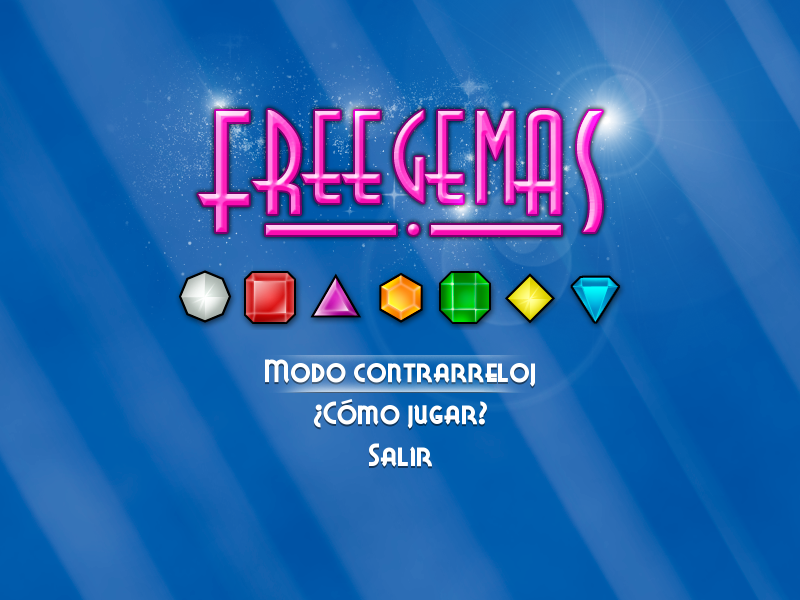
\includegraphics[width=0.49\textwidth]{imagenes/imagen_freegemas1}\hspace{0.1cm}
    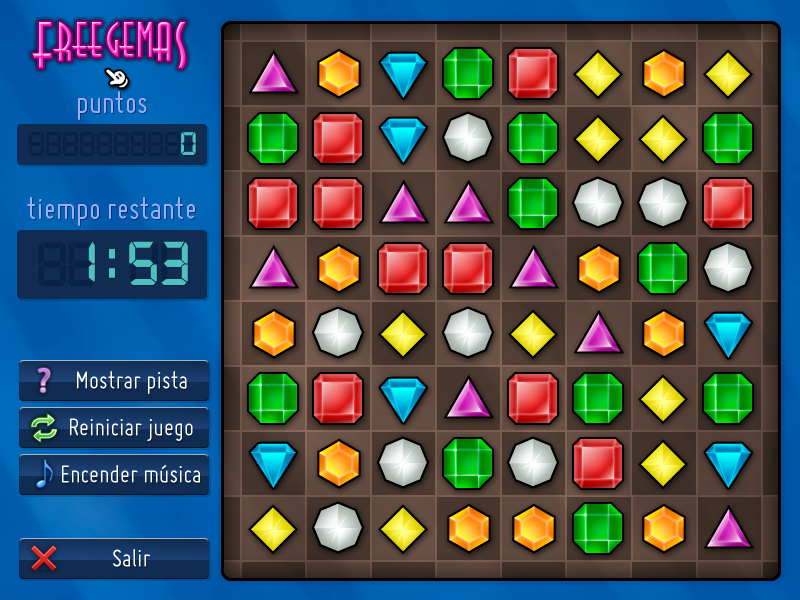
\includegraphics[width=0.49\textwidth]{imagenes/imagen_freegemas2}

    \medskip

    \begin{itemize}
    \item \textbf{Tres publicaciones} en Linux Magazine.
    \item \textbf{Inclusión oficial} en Guadalinex v8.
    \end{itemize}
  \end{center}
\end{frame}

\begin{frame}{Difusión}
  \begin{block}{Social media}
    \begin{itemize}
    \item Blog: \url{oflute.wordpress.com}, 5500 visitas en total.
    \item 3 vídeos en YouTube, aprox. 700 reproducciones.
    \end{itemize}    
  \end{block}

  \pause

  \begin{block}{Forja}
    \begin{itemize}
    \item \url{http://oflute.googlecode.com}
    \item Más de 270 revisiones.
    \item Aprox. 8000 líneas de código.
    \end{itemize}
  \end{block}

  \pause

  \begin{block}{Referencia del código}
    \begin{itemize}
    \item Generada con \textbf{Doxygen}.
    \item Disponible en la forja.
    \item Accesible en \url{http://www.josetomastocino.com/oflute}.
    \end{itemize}
  \end{block}
\end{frame}

\begin{frame}{Difusión}
  \begin{block}{Concurso Universitario de Software Libre}
    \begin{itemize}
    \item Mención especial a nivel nacional.
    \item Accésit al mejor proyecto de innovación en la fase local.
    \end{itemize}
  \end{block}
  
  \pause

  \begin{block}{Guadalinex}
    \begin{itemize}
    \item oFlute se encuentra  en los repositorios de \textbf{Guadalinex}.
    \end{itemize}
  \end{block}
\end{frame}
%%% Local Variables: 
%%% mode: latex
%%% TeX-master: "../presentacion"
%%% End: 


%\chapter{Manual del usuario}
%%
% Generado autom�ticamente por las hojas de estilo XSLT
% Modificado posteriormente a mano
%
% Antonio Garc�a Dom�nguez, (C) 2008
% nyoescape@gmail.com
% $Id$
%

\section{Instalaci�n de XMLEye}
\label{instPrograma}

 En este apartado cubrir� la instalaci�n de XMLEye en sus diferentes formas, tanto a nivel de usuario local como a nivel de sistema. Para instalar los conversores asociados y sus hojas de usuario y descriptores de formato, referirse al apartado~\ref{instHojas} (p�gina~\pageref{instHojas}). 

\subsection{Requisitos previos}

 Se necesita tener instalado un entorno Java compatible con J2SE 5.0 o superior. Su instalaci�n se realiza autom�ticamente si utilizamos los paquetes Debian. 

\subsubsection{Windows}

 Tendremos que ir a \url{http://java.sun.com/javase/downloads/index.jsp} y descargar una edici�n reciente del JRE de acuerdo a nuestro sistema operativo. Tanto si hemos obtenido la versi�n que no requiere conexi�n como la que descarga s�lo lo necesario a trav�s de Internet, todo lo que tendremos que hacer es ejecutar el instalador y seguir las instrucciones. 

\subsubsection{GNU/Linux}

 Si utilizamos una distribuci�n basada en Debian, podemos probar a instalar los paquetes \filename{icedtea\hyp{}7\hyp{}jre} o \filename{openjdk\hyp{}6\hyp{}jre}. OpenJDK es la iniciativa de Sun, que a fecha de hoy (03/07/2008) es pr�cticamente 100 \% libre salvo por algunas peque�as partes que el proyecto IcedTea ha reemplazado utilizando c�digo del proyecto GNU Classpath. Podemos instalar una versi�n de OpenJDK 6.0 con los reemplazos de IcedTea en Ubuntu 8.04 "Hardy Heron" y usarla como entorno Java por defecto con estas �rdenes: 

\begin{alltt}
	\command{sudo aptitude install openjdk-6-jre}
	\command{sudo update-alternatives --config java}
\end{alltt}

 Escogeremos la entrada de \filename{openjdk\hyp{}6\hyp{}jre} y pulsaremos Intro, terminando con este paso. Si estamos utilizando openSUSE 10.3, podemos usar sin problemas el entorno J2SE 5.0 de Sun que incluye de f�brica. En caso de que no estuviera instalado por alguna raz�n, tendr�amos que instalar los paquetes \filename{java\hyp{}1\_5\_0\hyp{}sun*} a trav�s del gestor de paquetes de YaST. 

\note{ Actualmente, OpenJDK sigue teniendo peque�os defectos en la forma en que sit�a los componentes Swing. Es posible que algunos di�logos tengan un aspecto distinto al normal, con botones demasiado grandes, por ejemplo. El JRE original de Sun no tiene estos problemas, pero no es 100 \% libre. De todas formas, los efectos de este problema son puramente est�ticos. }

\subsection{Instalaci�n desde distribuciones precompiladas}

\note{ Si se usa una distribuci�n basada en Debian, se deber�a considerar el uso de los paquetes Debian, que son mucho m�s c�modos de usar. }

\subsubsection{Un �nico usuario, GNU/Linux}

 El proceso es muy sencillo: s�lo hay que descargar el \filename{\hyp{}dist\hyp{}tar.gz} m�s reciente de XMLEye de \url{https://forja.rediris.es/frs/?group_id=233} y descomprimirlo bajo nuestro directorio personal. Para ejecutar XMLEye, basta con ejecutar el gui�n \filename{/home/\-\emph{usuario}/\-xmleye/\-xmleye} tras pulsar la combinaci�n \keycombo{ALT + F2}. Una opci�n m�s c�moda para los habituales de la l�nea de �rdenes es a�adir la siguiente l�nea a \filename{\~\{\}/\-.bashrc}: 

\begin{alltt}
export PATH=\$PATH:\~{}/xmleye
\end{alltt}

 Haciendo esto, se puede abrir cualquier documento compatible desde la l�nea de �rdenes mediante: 

\begin{alltt}
xmleye \emph{(ruta absoluta o relativa)}
\end{alltt}

 Seg�n este procedimiento, las hojas de usuario se instalar�n en \filename{/home/\-\emph{usuario}/\-xmleye/\-xslt}, y los descriptores de formatos en \filename{/home/\-\emph{usuario}/\-xmleye/\-formats}. Las opciones se guardar�n en \filename{/home/\-\emph{usuario}/\-xmleye}. 

\subsubsection{M�ltiples usuarios, GNU/Linux}

 Un caso m�s complejo es cuando queremos instalarlo para varios usuarios, pero queremos tener ajustes distintos para cada usuario (las hojas son comunes a todos). Al igual que en el caso anterior, deberemos tener instalado un JRE compatible con J2SE 5.0 o superior antes que nada, pero despu�s usaremos una distribuci�n diferente de los ficheros. 

 La distribuci�n "ideal" ser�a la del paquete Debian, pero como es un poco m�s compleja de lo que necesitamos, nos limitaremos a un t�rmino medio. Primero descomprimiremos la �ltima distribuci�n de XMLEye (el enlace de descarga est� en la secci�n anterior) a \filename{/opt}, que crearemos si no existe ya: 

\begin{alltt}
sudo mkdir /opt
cd /opt
sudo tar xjf \emph{(ruta a distribuci�n)}

\end{alltt}

 Tendremos que retocar el gui�n de lanzamiento un poco. XMLEye cuenta con dos variables de entorno, \envar{XMLEYE\_PREF\_DIR} y \envar{XMLEYE\_FORMATS\_DIR}, que indican la ruta en la que se guardar�n las preferencias y los formatos personalizados por el usuario. Adem�s, XMLEye supone que las hojas de usuario se hallan bajo el subdirectorio \filename{xslt} de la ruta sobre la cual es lanzado. 

 Teniendo todo esto en cuenta, habr� que sustituir las l�neas que afectan a \envar{PROGRAM\_DIR} y \envar{PROGRAM\_JAR} por: 

\begin{alltt}
PROGRAM\_DIR=/opt/xmleye
PROGRAM\_JAR=xmleye.jar
export XMLEYE\_PREF\_DIR=\${HOME}/.xmleye
export XMLEYE\_FORMATS\_DIR=\${HOME}/.xmleye
mkdir -p \${XMLEYE\_PREF\_DIR}
\end{alltt}

 De forma similar a la secci�n anterior, los usuarios podr�an directamente ejecutar XMLEye a trav�s de la ruta completa. Para que todos los usuarios puedan ejecutar XMLEye por nombre, se puede a�adir esta l�nea a \filename{/etc/\-environment}: 

\begin{alltt}
export PATH=\$PATH:/opt/xmleye
\end{alltt}

 Si queremos que aparezca una entrada de men� y que se asocien los ficheros XML con XMLEye, entonces tendremos que, adem�s de seguir el paso anterior, crear el fichero \filename{/usr/\-share/\-applications/\-xmleye.desktop} con este contenido: 

\begin{alltt}
[Desktop Entry]
Encoding=UTF-8
Version=1.0
Type=Application
Terminal=false
Exec=xmleye  \%U
Comment[es]=Visor gen�rico de XML dirigido por datos
Name=XMLEye
Comment=Generic data-driven XML Viewer
GenericName=Generic XML viewer
GenericName[es]=Visor gen�rico de XML
Icon=accessories-text-editor
Categories=Utility;TextEditor;
MimeType=application/xml;
\end{alltt}

 Actualizaremos las bases de datos y reiniciaremos los men�s de GNOME con: 

\begin{alltt}
sudo update-desktop-database
sudo update-menus
sudo killall gnome-panel nautilus
\end{alltt}

 Ya deber�a de aparecer la entrada de XMLEye en el men� principal de GNOME. 

 Las hojas de usuario estar�n bajo \filename{/opt/\-xmleye/\-xslt}, y los descriptores de formato en \filename{/opt/\-xmleye/\-formats}. 

\subsubsection{Windows}

 Descargamos y descomprimimos en alguna carpeta el \filename{\hyp{}dist\hyp{}tar.gz} m�s reciente de XMLEye de \url{https://forja.rediris.es/frs/?group_id=233}. 

 Para ejecutar XMLEye, haremos doble clic en el fichero \filename{xmleye.jar} de la carpeta en que hemos descomprimido la distribuci�n. 

\subsection{Instalaci�n desde paquetes Debian}

 Esta es la opci�n a seguir siempre que sea posible, ya que adem�s de ser m�s sencilla, permitir� recibir actualizaciones de forma autom�tica. 

 Los paquetes han sido desarrollados para Ubuntu Gutsy, pero deber�an funcionar en cualquier distribuci�n basada en Debian reciente. 

 Los pasos a seguir son: 

\begin{enumerate}
\item Descargaremos la firma digital de los paquetes disponible bajo \url{http://www.shoyusauce.org/packages/claveDebian.asc}.

\item  A�adiremos la firma al anillo de confianza de Apt. En primer lugar lanzaremos la opci�n \emph{Sistema $\rightarrow$ Administraci�n $\rightarrow$ Or�genes
	  de software} bajo el men� principal de GNOME. 

 Hecho esto, seleccionaremos la pesta�a \guilabel[moreinfo = none]{Autentificaci�n} y pulsaremos en el bot�n \guibutton[moreinfo = none]{Importar clave...}, tras lo cual seleccionaremos la firma que antes descargamos. 

 A�n no cerraremos la ventana: nos queda una cosa por hacer. 

\item  Ahora a�adiremos los repositorios de paquetes binarios y paquetes de fuentes de \application{XMLEye} y sus hojas de estilos. Esta vez iremos a la pesta�a \guilabel[moreinfo = none]{Software de terceros}. 

 Pulsaremos en \guibutton[moreinfo = none]{A�adir} e introduciremos esta l�nea tal y como est�: 

\begin{alltt}
deb http://www.shoyusauce.org/packages/ubuntu/ gutsy main
\end{alltt}

 Volvemos a pulsar en \guibutton[moreinfo = none]{A�adir}, pero esta vez introducimos esta l�nea: 

\begin{alltt}
deb-src http://www.shoyusauce.org/packages/ubuntu/ gutsy main
\end{alltt}

 Ya podemos pulsar en \guibutton[moreinfo = none]{Cerrar} para cerrar este di�logo, y solicitar la actualizaci�n de nuestras listas de paquetes en el di�logo subsecuente pulsando en \guibutton[moreinfo = none]{Recargar}. Una vez haya terminado, estaremos listos para instalar \application{XMLEye} y otros paquetes de apoyo, como \application{pprocACL2}. 

\item  Lanzaremos \emph{Sistema $\rightarrow$ Administraci�n $\rightarrow$ Gestor
	  de paquetes Synaptic} y pulsaremos en el bot�n \guibutton[moreinfo = none]{Buscar} de la barra de herramientas. 

 Introduciendo "xmleye" en el campo de b�squeda obtendremos un �nico resultado en el que podremos hacer doble clic para marcar para su instalaci�n. Tambi�n podr�amos seleccionar otros paquetes con los conversores, descriptores y hojas de estilos espec�ficas de otros formatos, como "libacl2-procesador-perl" o "libyaxml-reverse-perl", de la misma forma. 

 Una vez todos los paquetes que deseamos instalar se hallen marcados, pulsaremos en \guibutton[moreinfo = none]{Aplicar} de la barra de herramientas para confirmar los cambios. 

\item  �Listo! Ya podemos lanzar XMLEye a trav�s de \emph{Aplicaciones $\rightarrow$ Accesorios $\rightarrow$ XMLEye} del men� principal de GNOME. 

\note{ S�lo un detalle: todas las opciones que establezcamos ir�n a parar al subdirectorio \filename{.xmleye} bajo nuestro directorio personal, es decir, \filename{/home/\-\emph{nombredeusuario}}. }

\end{enumerate}

 La ruta bajo la cual tendremos que instalar las hojas de usuario ser� \filename{/usr/\-share/\-xmleye/\-xslt}, y en \filename{/usr/\-share/\-xmleye/\-formats} se hallar�n los descriptores de formato. 

\subsection{Compilaci�n del c�digo fuente}

\note{ Aunque hay instant�neas disponibles del c�digo fuente, �stas son m�s para los usuarios que los desarrolladores. En caso de querer participar como desarrollador, recomiendo encarecidamente usar una copia de trabajo del repositorio Subversion. Bastar� con instalar el paquete \filename{subversion} y seguir algunas instrucciones sencillas. Para m�s informaci�n, v�ase el excelente libro~\cite{svnhandbook}. }

 Tras obtener un JDK compatible con J2SE 5.0 o superior, como el de OpenJDK 6.0 o 7.0, IcedTea 6.0 o 7.0, o los originales de Sun, tendremos que instalar adem�s la herramienta Apache Ant y el entorno de pruebas de unidad JUnit, en una de sus versiones 3.X. En Ubuntu 8.04 "Hardy Heron", esto se puede hacer mediante: 

\begin{alltt}
sudo aptitude install openjdk-6-jdk ant junit
\end{alltt}

 Ahora tendremos que crear una copia de trabajo local de la �ltima revisi�n de la rama principal de desarrollo del repositorio de RedIris: 

\begin{verbatim}
svn checkout \
  https://forja.rediris.es/svn/csl2-xmleye/XMLEye/trunk \
  xmleye
\end{verbatim}

 Ya podemos introducirnos en \filename{xmleye} y aprovechar los objetivos ya definidos en el fichero \filename{build.xml} de Ant. Si se desea instalar \filename{xmleye} a partir de fuentes, se recomienda usar el objetivo \varname{dist} e instalar la distribuci�n seg�n alguno de los m�todos antes expuestos. 

\begin{description}
\item[clean] \mbox{}
Limpia el �rbol de directorios existente.

\item[compile] \mbox{}
Compila todo el c�digo fuente.

\item[dist] \mbox{}
Compila las fuentes ,ejecuta las pruebas de unidad y genera una distribuci�n autocontenida en el subdirectorio \filename{dist}.

\item[dist-jar] \mbox{}
Tras compilar y ejecutar las pruebas de unidad, genera un fichero \filename{.jar} bajo \filename{dist}, pero no llega a empaquetarlo con todo lo dem�s.

\item[docs] \mbox{}
Genera la documentaci�n del API en formato HTML en el subdirectorio \filename{docs} a trav�s de Javadoc.

\item[run] \mbox{}
Se trata del objetivo por defecto (ejecutado a trav�s de \command{ant}). Compila el c�digo y ejecuta la versi�n as� compilada de XMLEye.

\item[run-about] \mbox{}
Compila el c�digo y ejecuta �nicamente la ventana de "Acerca de". �til a la hora de dise�ar la interfaz.

\item[run-find] \mbox{}
Como la anterior, pero para el di�logo de b�squeda.

\item[run-types] \mbox{}
M�s de lo mismo, pero para el di�logo de edici�n de tipos.

\item[test] \mbox{}
Ejecuta las pruebas de unidad. La salida de cada conjunto de pruebas se halla bajo el fichero \filename{TEST\hyp{}*} correspondiente.

\end{description}

 M�s cosas a tener en cuenta: esta aplicaci�n depende de InfoNode Tabbed Panel 1.5.0 (licenciado bajo la GPL para uso no comercial) y del look and feel JGoodies Looks 2.1.4 (licenciado bajo BSD), disponibles en \url{http://www.infonode.net/index.html?itp} y \url{https://looks.dev.java.net/} respectivamente. De todas formas, los ficheros \filename{.jar} necesarios se hallan en el propio repositorio, por lo que no hay que hacer nada al respecto. 

 Adem�s, el desarrollo puede hacerse mucho m�s c�modamente si se emplea el plugin Subclipse para Eclipse, disponible en \url{http://subclipse.tigris.org/}, y se importa a trav�s de �l el proyecto Eclipse desde el repositorio. As� podemos contar con sus funcionalidades de refactorizaci�n y notificaci�n de errores y avisos de compilaci�n en directo. 

\section{Instalaci�n de conversores asociados}

\label{instHojas}

\subsection{\nombrepostprocesador{}: convertidor de demostraciones de ACL2}

 Como muestra de las capacidades de XMLEye, desarroll� en paralelo un conjunto de hojas de usuario de preprocesado y visualizaci�n, junto con un tipo de documento para ACL2. Esto nos permite demostraciones para dicho sistema en formato \filename{.lisp} siguiendo una estructura arb�rea donde cada nodo se muestra como un hipertexto con enlaces a otras partes de la demostraci�n. 

 La subcarpeta \filename{t/\-testInputs} del fichero de fuentes con nombre de la forma \filename{ACL2\hyp{}Procesador\hyp{}*.tar.gz} m�s reciente contiene algunos ejemplos de inter�s, extra�dos de tutoriales reales de aprendizaje del uso de ACL2. 

 Primero nos ocuparemos de las dependencias, y luego veremos tres formas de instalar el convertidor, el descriptor de formato y las hojas de usuario. 

\subsubsection{Dependencias}

Las dependencias a instalar variar�n seg�n el m�todo de instalaci�n.

\paragraph{ACL2 2.9 o superior}

 Se ha depurado \postprocesador{} tambi�n con ACL2 3.1 y 3.3. 

\subparagraph{GNU/Linux}

En una distribuci�n basada en Debian, instalar ACL2 es tan sencillo como ejecutar la siguiente orden (necesitamos \application{gcc} para poder certificar libros):

\begin{alltt}
\command{sudo aptitude install acl2 gcc}
\end{alltt}

Otras distribuciones requerir�n del proceso manual de instalaci�n, documentado bajo \url{http://www.cs.utexas.edu/users/moore/acl2/v3-3/installation/installation.html}. Es sencillo, pero la compilaci�n de los libros puede llevar mucho tiempo (alrededor de 8-10 horas).

\subparagraph{Windows}

Descargaremos e instalaremos la distribuci�n completa de ACL2 preparada por Jared Davis, disponible en \url{http://www.cs.utexas.edu/users/moore/acl2/v3-3/distrib/windows/}. Incluye todo lo que podr�amos necesitar para trabajar con ACL2:

\begin{itemize}
\item ACL2 3.3

\item GCL 2.6.7, el entorno Lisp que necesitamos, junto con el compilador GCC necesario para certificar libros.

\item El editor GNU Emacs en su versi�n 21.3.

\item Documentaci�n de ACL2.

\item Una colecci�n de libros previamente certificados.

\end{itemize}

\paragraph{Perl 5.8.6 o superior}
\label{inst_perl}
\subparagraph{GNU/Linux}

 La gran mayor�a de las distribuciones lo incluyen de f�brica, pero en el caso en que no lo tuvi�ramos, podr�amos instalarlo en una distribuci�n basada en Debian con: 

\begin{alltt}
\command{sudo aptitude install perl}
\end{alltt}

Otra opci�n ser�a descargar el c�digo fuente de \url{http://www.perl.com/download.csp} y compilarlo, pero no se cubrir� dicha alternativa aqu�.

\subparagraph{Windows}

 Utilizaremos la edici�n 5.10 m�s reciente de Strawberry Perl, disponible bajo \url{http://strawberryperl.com/}. S�lo hemos de seguir los pasos del instalador. 

\paragraph{M�dulos Perl: \application{PAR}}
\label{inst_par}
 Una vez hayamos instalado Perl (v�ase la secci�n ), s�lo necesitamos ejecutar una orden m�s. No es necesario seguir la configuraci�n manual del acceso a CPAN en ninguno de los dos casos. 

\subparagraph{GNU/Linux}

\begin{alltt}
\command{sudo cpan PAR}
\end{alltt}

\subparagraph{Windows}

\begin{alltt}
\command{cpan PAR}
\end{alltt}

\paragraph{M�dulos Perl: \application{PAR::Packer}}
\label{inst_parpacker}
\subparagraph{GNU/Linux}

 Si estamos usando una distribuci�n basada en Debian reciente, podemos ejecutar: 

\begin{alltt}
\command{sudo aptitude install libpar-packer-perl}
\end{alltt}

 De lo contrario, ejecutaremos: 

\begin{alltt}
\command{sudo cpan PAR::Packer}
\end{alltt}

\subparagraph{Windows}

 Tendremos que obtener la �ltima copia del c�digo fuente de \application{PAR::Packer} del repositorio SVN, ya que la versi�n m�s reciente en el CPAN a d�a de hoy (03/07/2008), la 0.980, no incluye el arreglo de un defecto que imposibilitaba su instalaci�n en Strawberry Perl. Para ello, instalaremos el cliente Subversion TortoiseSVN, disponible bajo \url{http://tortoisesvn.tigris.org/}, y haremos un \emph{checkout} de la direcci�n \url{http://svn.openfoundry.org/par/PAR-Packer/trunk/}. 

 Una vez hayamos descargado el c�digo, abriremos una ventana del int�rprete de �rdenes, y dentro del directorio con el c�digo fuente, ejecutaremos: 

\begin{alltt}
\computeroutput{perl Makefile.PL
dmake
dmake test
dmake install
}
\end{alltt}

 Si se nos pide instalar alguna dependencia en alguno de los pasos, aceptaremos. 

\paragraph{Biblioteca \application{libxml2}}
\label{inst_xml}
\subparagraph{GNU/Linux}

 Si estamos usando una distribuci�n basada en Debian, ejecutaremos esta orden: 

\begin{alltt}
\command{sudo aptitude install libxml2-dev}
\end{alltt}

\subparagraph{Windows}

 No hay que hacer nada: viene ya incluida con Strawberry Perl. 

\subsubsection{Instalaci�n mediante paquetes Debian}

 Si instalamos XMLEye mediante el paquete Debian, s�lo tendremos que instalar el paquete \filename{libacl2\hyp{}procesador\hyp{}perl}. La pr�xima vez que iniciemos XMLEye tendremos todo lo necesario a nuestra disposici�n, incluido ACL2. 

\subsubsection{Instalaci�n desde distribuci�n monol�tica}
\label{inst_distrib_monolit}
 Necesitaremos previamente haber instalado ACL2, y haber instalado XMLEye descomprimiendo la distribuci�n de la forja. Descargaremos del �rea de ficheros (\url{http://forja.rediris.es/frs/?group_id=233}) de la forja de XMLEye el fichero \filename{ACL2\hyp{}Procesador\hyp{}*\hyp{}standalone\hyp{}*.tar.gz} m�s reciente que se corresponda con la microarquitectura de nuestra CPU y nuestro sistema operativo, y lo descomprimiremos sobre el directorio en el que instalamos XMLEye. 

\subsubsection{Instalaci�n desde distribuci�n basada en PAR}
\label{inst_distrib_par}
 Necesitaremos ACL2, Perl y el m�dulo PAR. El proceso es id�ntico al de~\ref{inst_distrib_monolit} (p�gina~\pageref{inst_distrib_monolit}), pero en este caso el fichero a descargar y descomprimir es \filename{ACL2\hyp{}Procesador\hyp{}*\hyp{}par\hyp{}noarch.tar.gz}, que es independiente de la CPU y el sistema operativo escogido. 

\subsubsection{Instalaci�n manual a partir de fuentes}
\label{inst_fuentes}
 Los pasos, tras instalar todas las dependencias, son los siguientes: 

\begin{enumerate}
\item Descomprimimos el fichero de fuentes bajo \filename{/tmp}, y nos introducimos en sus contenidos:

\begin{alltt}
cd /tmp
tar xzf \emph{(ruta a las fuentes)}
cd ACL2-Procesador-*
\end{alltt}

\item Instalamos el preprocesador tal y como instalar�amos cualquier paquete Perl. Este proceso resultar� muy familiar a cualquier usuario de las \application{autotools}:

\begin{alltt}
perl Makefile.PL
sudo make
make test
sudo make install
\end{alltt}

 Es muy probable que Perl nos solicite en la primera orden instalar algunas dependencias. Siempre le diremos que s�. La �ltima orden se podr�a sustituir por \command{sudo checkinstall} si deseamos poder desinstalarlo f�cilmente, instalando \postprocesador{} como un paquete Debian. 

\item  Lo siguiente es instalar las hojas de usuario, que es tan f�cil (suponiendo que la ruta de hojas de usuario es \filename{/home/\-\emph{tunombredeuaurio}/\-xmleye/\-xslt} como: 

\begin{alltt}
cp -r xslt/* \$HOME/xmleye/xslt
\end{alltt}

\item  Terminaremos instalando el descriptor de tipo a su sitio: 

\begin{alltt}
cp types/* \$HOME/xmleye/types
\end{alltt}

\end{enumerate}

\subsubsection{Ejecuci�n independiente de XMLEye}
\label{ejecucion}
 Podemos comproabr que todo va bien ejecutando el gui�n principal. La forma de hacerlo variar� seg�n el m�todo de instalaci�n usado: 

\begin{itemize}
\item Desde el paquete Debian, o desde fuentes: \command{pprocACL2} desde cualquier ruta.

\item Desde la distribuci�n monol�tica: \command{\emph{(ruta)}/\-pprocACL2}, utilizando la ruta bajo la cual se halla instalado XMLEye. Podr�amos a�adir esta ruta al PATH si quisi�ramos.

\item Desde la distribuci�n basada en PAR: \command{perl -MPAR (ruta)/\-pprocACL2.par}, utilizando la ruta bajo la cual se halla instalado XMLEye.

\end{itemize}

 Deber�amos obtener una salida como la que viene a continuaci�n. Por razones t�cnicas, es posible que en ciertos entornos la distribuci�n basada en PAR no produzca ninguna salida, pero esto no es un problema: seguir� funcionando de forma normal una vez le pasemos un fichero de entrada, imprimi�ndose el XML resultante por salida est�ndar, y los mensajes de estado por la salida de errores. 

\begin{alltt}
\computeroutput{Usage:
  pprocACL2 [opciones] [entrada Lisp ACL2]

Options:
  --help, -h, -?
          Se limita a mostrar un mensaje corto de ayuda.

  --man, -m
          Muestra un mensaje detallado de ayuda en formato man.}
\end{alltt}

\subsection{\nombreyaxml{}: conversor de documentos YAML a XML}

 Este otro conversor se desarroll� para abrir con XMLEye la familia completa de documentos con lenguajes basados en YAML 1.1 o JSON. Al igual que \postprocesador{}, incorpora las hojas de usuario y descriptores de formatos necesarios para su funcionamiento. Incluye soporte para anclias y alias de YAML. 

 Tambi�n en este caso se pueden ver algunos ejemplos de entradas aceptadas en \filename{t/\-testInputs} de las fuentes, disponibles como ficheros con nombres del estilo de \filename{YAXML\hyp{}Reverse\hyp{}*.tar.gz} en el �rea de ficheros de la forja (\url{http://forja.rediris.es/frs/?group_id=233}). 

 Para evitar repeticiones innecesarias, aprovecharemos las instrucciones de instalaci�n de algunas de las dependencias y algunos de los pasos de los m�todos de instalaci�n de \postprocesador{}. Comentaremos �nicamente los aspectos que cambian. 

\subsubsection{Dependencias}

Hay algunas dependencias de \application{YAXML::Reverse} cuyos m�todos
de instalaci�n ya se han mencionado en la secci�n \S\ref{inst_perl}
an�loga de \postprocesador{}:

\begin{description}
\item[Perl] \mbox{}
V�ase la p�gina~\pageref{inst_perl}.

\item[PAR] \mbox{}
V�ase la p�gina~\pageref{inst_par}.

\item[PAR::Packer] \mbox{}
V�ase la p�gina~\pageref{inst_parpacker}.

\item[Bibliotecas XML] \mbox{}
V�ase la p�gina~\pageref{inst_xml}.

\end{description}

\paragraph{Bibliotecas XSLT}

 Tambi�n puede que nos hagan falta las bibliotecas para XSLT. Dependiendo del sistema operativo sobre el que trabajemos, los m�todos de instalaci�n cambiar�n. 

\subparagraph{GNU/Linux}

 Necesitaremos instalar los paquetes de desarrollo para las bibliotecas \application{exslt}, \application{gdbm} y \application{gcrypt}. En una distribuci�n basada en Debian, usaremos: 

\begin{alltt}
\computeroutput{sudo aptitude install libexslt-dev \textbackslash{}
                      libgdbm-dev  \textbackslash{}
                      libgcrypt-dev}
\end{alltt}

\subparagraph{Windows}

 Como instalar manualmente las bibliotecas es demasiado complejo, usaremos una distribuci�n precompilada del m�dulo \application{XML::LibXSLT}. Para ello, ejecutaremos esta orden bajo la interfaz de l�nea de �rdenes: 

\begin{alltt}
\computeroutput{ppm install XML::LibXSLT}
\end{alltt}

\subsubsection{Instalaci�n mediante paquetes Debian}

Una vez instalemos XMLEye mediante el paquete Debian, s�lo habr� que instalar el paquete \filename{libyaxml\hyp{}reverse\hyp{}perl}, cerrar y volver a abrir XMLEye y todo quedar� listo.

\subsubsection{Instalaci�n desde distribuci�n monol�tica}

 En este caso utilizaremos el fichero m�s reciente que concuerde con nuestro entorno que siga el patr�n \filename{YAXML\hyp{}Reverse\hyp{}*\hyp{}standalone\hyp{}*.tar.gz}. 

\subsubsection{Instalaci�n desde distribuci�n basada en PAR}

 Esta vez las distribuciones (que siguen el patr�n \filename{YAXML\hyp{}Reverse\hyp{}*\hyp{}par\hyp{}*.tar.gz}) ser�n espec�ficas del entorno, pero por lo dem�s es todo igual. 

\subsubsection{Instalaci�n manual a partir de fuentes}

 El patr�n del nombre de fichero cambia a \filename{YAXML\hyp{}Reverse\hyp{}*.tar.gz} m�s reciente, y no se necesita ACL2, sino las bibliotecas de XSLT. El resto de las dependencias siguen siendo necesarias.

\subsubsection{Ejecuci�n independiente de XMLEye}

 El proceso es an�logo al de la secci�n~\ref{ejecucion} (p�gina~\pageref{ejecucion}), pero esta vez el gui�n principal es \filename{yaml2xml} (y el PAR es \filename{yaml2xml.par}), y la salida que deber�amos obtener tendr�a que ser similar a �sta: 

\begin{alltt}
\prompt{\$ yaml2xml}

\computeroutput{yaml2xml, using YAXML::Reverse 0.3.4
Usage: yaml2xml [path to .yaml]}
\end{alltt}

\subsection{Instrucciones gen�ricas}

 Estas instrucciones son las m�s detalladas, y sirven para cualquier hoja de usuario disponible actualmente y en el futuro, siempre que no var�e el dise�o de XMLEye. 

\subsubsection{Instalaci�n de hojas de usuario}

 Una hoja de usuario nos permite mejorar XMLEye en una de las siguientes formas: 

\begin{itemize}
\item Ver la estructura de un documento XML de otra forma. Un ejemplo ser�a ver s�lo un resumen del documento, cambiar el orden para su preprocesamiento, o decorar los nodos del �rbol con nuevas etiquetas e iconos.

\item Ver el contenido de un nodo del documento de otra forma. Podemos hacer cualquier cosa que se nos ocurra con XHTML 1.1 y CSS (no hay soporte para Javascript), y establecer v�nculos entre nodos del �rbol y nodos de otros documentos.

\end{itemize}

 Realmente, no son m�s que conjuntos de hojas XSLT que siguen una determinada estructura para permitir su localizaci�n y su integraci�n con otras hojas, ya que una hoja de usuario puede ser una especializaci�n de otra hoja. 

 La ruta donde se guardan las hojas de usuario variar� dependiendo del m�todo de instalaci�n que hayamos seguido. Para m�s detalles, referirse al apartado~\ref{instPrograma} (p�gina~\pageref{instPrograma}). Nos encontraremos bajo dicha ruta una serie de ficheros (s�lo de inter�s para desarrolladores) y dos subdirectorios, \filename{preproc} y \filename{view}, en cuyo interior habr� un subdirectorio por hoja de usuario de preprocesado o visualizaci�n, respectivamente. 

 Instalar una hoja de usuario no es m�s entonces que asegurarnos que su subdirectorio se halle en el lugar correcto, y reiniciar XMLEye. Encontraremos entradas con los mismo nombres que los subdirectorio correspondientes en las entradas \emph{Preferencias $\rightarrow$ Preprocesamiento} y \emph{Preferencias $\rightarrow$ Visualizaci�n} de XMLEye. Por defecto tendremos instalado como m�nimo las hojas de usuario de preprocesado y visualizaci�n \filename{xml}, y la hoja de visualizaci�n \filename{xmlSource} a partir de la versi�n 1.22. 

\subsubsection{Instalaci�n de nuevos formatos de documentos}

 A pesar de su nombre, XMLEye puede visualizar documentos de cualquier formato, usando un conversor si no se trata de un documento XML originalmente, e integrarse con su editor (monitorizando el fichero en busca de cambios) siempre que se le d� la informaci�n correspondiente. Esa informaci�n viene integrada en un \emph{descriptor de formato de documento}. 

 Dichos descriptores se nombran usando la extensi�n \filename{.format} y siguen un formato XML sencillo, en cuyos detalles no entraremos aqu� (v�ase el Manual del Desarrollador). Lo �nico que nos importa es su instalaci�n, que es tan sencilla como copiar el fichero \filename{.format} correspondiente a la ruta de tipos que le corresponde seg�n el tipo de instalaci�n que hayamos realizado. 

 Una vez instalado y reiniciado XMLEye, podremos abrir cualquier documento que tenga las extensiones especificadas en el tipo de documento instalado sin m�s problemas, siempre que su editor y preprocesador (si tiene alguno) se hallen debidamente instalados y tengan �rdenes que puedan ejecutarse desde el directorio principal de XMLEye (posiblemente usando ejecutables bajo los directorios dentro de la variable de entorno \envar{PATH}). 

\section{Uso y configuraci�n}
\label{uso}
Este apartado de la gu�a trata acerca del empleo de XMLEye y de su configuraci�n. Para cuestiones relacionadas con la instalaci�n o con detalles de implementaci�n, referirse a los apartados anteriores o al Manual del Desarrollador, respectivamente.

A lo largo de esta gu�a nos referiremos exclusivamente a las opciones de los men�s, pero pr�cticamente toda acci�n tiene una combinaci�n equivalente en el teclado,indicada en la parte derecha del elemento del men� correspondiente (y si no, es un fallo del que se agradecer�a una notificaci�n ;-): informe de �l en \url{https://forja.rediris.es/tracker/?group_id=233} ). Adem�s, las opciones m�s comunes poseen un bot�n en la barra de herramientas, cuyo icono es una versi�n ampliada del icono de la entrada de men� correspondiente.

Podemos cambiar entre los botones de la barra de herramientas, el �rbol y el navegador mediante \keycombo{Ctrl + Tab} en de izquierda a derecha y de arriba abajo, o mediante \keycombo{Shift + Ctrl + Tab} en direcci�n inversa.\keycombo{Tab} y \keycombo{Shift + Tab} siguen funcionando tambi�n de la forma usual, pero se hallan redefinidos en el navegador para navegar por los hiperv�nculos.

La forma de lanzar el programa se detalla en la gu�a de instalaci�n, y variar� seg�n el m�todo seguido.

\subsection{Apertura y edici�n de documentos}

 Bajo el men� \guimenu[moreinfo = none]{Fichero}, disponemos de \guimenuitem[moreinfo = none]{Abrir...}, en donde podremos seleccionar un fichero de cualquier tipo, o uno de los formatos que tengamos instalados. 

 Una vez hayamos seleccionado el fichero, XMLEye detectar� a partir de la extensi�n de qu� formato se trata y aplicar� el convertidor indicado, si lo hay. Una vez el fichero se halle disponible en formato XML, pasar� por la hoja de preprocesado y se mostrar� su �rbol en pantalla junto con la visualizaci�n de su nodo ra�z. 

 Para editar el fichero fuente con el editor definido en el descriptor de formato, usaremos \guimenuitem[moreinfo = none]{Editar fuente}. Si \emph{Preferencias $\rightarrow$ Actualizaci�n
      autom�tica} se halla activo, XMLEye monitorizar� el fichero en segundo plano y actualizar� el �rbol XML cada vez que se produzcan cambios en �l, indpendientemente de si estuviera o no el editor abierto. 

 Por �ltimo, podemos acceder a los 5 �ltimos documentos abiertos con �xito, o \guimenuitem[moreinfo = none]{Salir} del programa. 

 Para cerrar un documento, actualmente no hay ninguna entrada en el men� \guimenu[moreinfo = none]{Fichero}, pero puede hacerse pulsando la cruz de su pesta�a correspondiente. Para cerrar todos los documentos, podemos pulsar en el bot�n de cierre general en el extremo derecho del componente de pesta�as. 

\subsection{Navegaci�n por los documentos}

 El documento XML tras ser preprocesado sigue una estructura arb�rea normal y corriente, por lo que podemos realizar las acciones usuales mediante las entradas del men� \guimenu[moreinfo = none]{Navegar}. En particular: 

\begin{description}
\item[Buscar...] \mbox{}
 Abre un di�logo de b�squeda en el que podemos buscar siguiendo diversos par�metros. Adem�s de las opciones usuales de b�squeda por palabras completas o por concordancia de may�sculas, se puede marcar el �mbito de la b�squeda. 

\item[Buscar siguiente] \mbox{}
 Repite la �ltima b�squeda realizada, mostrando un error en caso de que no se halla realizado una anteriormente. Si hemos llegado al �ltimo resultado de la �ltima b�squeda, volveremos al primero despu�s. 

 La repetici�n de una b�squeda es muy r�pida, ya que XMLEye se ocupa de almacenar los resultados tras la primera petici�n y va dando directamente los resultados que le siguen dispu�s. 

\item[Padre] \mbox{}
 Sube un nivel en la jerarqu�a del �rbol, o no hace nada si estamos en la ra�z. 

\item[Hijo] \mbox{}
 Baja un nivel en la jerarqu�a del �rbol, o no hace nada si estamos en un nodo hoja. 

\item[Hermano anterior] \mbox{}
 Se desplaza al anterior nodo hijo del padre del nodo actual, o no hace nada si estamos en su primer hijo. 

\item[Hermano siguiente] \mbox{}
 Se desplaza al siguiente nodo hijo del padre del nodo actual, o no hace nada si estamos en su �ltimo hijo. 

\item[Expandir todo] \mbox{}
 Expande el contenido de todos los nodos del �rbol, de tal forma que todo nodo quede directamente visible, a menos que haya sido ocultado expl�citamente por la hoja de visualizaci�n. 

\item[Contraer todo] \mbox{}
 Contrae el contenido de todos los nodos del �rbol, de tal forma que �nicamente el nodo ra�z quede visible. 

\end{description}

Aunque casi toda acci�n es accesible mediante rat�n, se recomienda
aprender los accesos directos mediante teclado, ya que agilizan
enormemente los desplazamientos. En la tabla \ref{teclado_arbol}
(p�gina~\pageref{teclado_arbol}) se listan todos los accesos directos
mediante teclado para navegar por el �rbol del documento, tras hacer
clic en �l.

\begin{table}
\centering
\begin{tabularx}{\textwidth}{| c | X |} 
\hline
Combinaci�n de teclas & \multicolumn{1}{c|}{Efecto} \\ \hline
\hline
\keycombo{Arriba} & Selecciona el nodo anterior en la vista actual del �rbol. \\ \hline
\keycombo{Abajo} & Selecciona el nodo siguiente en la vista actual del �rbol. \\ \hline
\keycombo{Izquierda} & Sube al nodo padre si el nodo est� cerrado, y cierra el nodo actual de lo contrario. \\ \hline
\keycombo{Derecha} & Abre el nodo actual si est� cerrado, y baja al primer hijo de lo contrario. \\ \hline
\keycombo{Inicio} & Selecciona el primer nodo en la vista actual del �rbol. \\ \hline
\keycombo{Fin} & Selecciona el �ltimo nodo en la vista actual del �rbol. \\ \hline
\keycombo{Alt + Arriba} & Selecciona al nodo padre del actual. \\ \hline
\keycombo{Alt + Abajo} & Selecciona al primer hijo del nodo actual. \\ \hline
\keycombo{Alt + Izquierda} & Selecciona al hermano anterior del nodo actual. \\ \hline
\keycombo{Alt + Derecha} & Selecciona al hermano siguiente del nodo actual. \\ \hline

\end{tabularx}
\caption{Accesos de teclado para navegaci�n por el �rbol}
\label{teclado_arbol}
\end{table}
 Podemos cambiar entre los documentos haciendo clic en sus pesta�as correspondientes, o pulsando en la flecha hacia abajo justo a la izquierda de la cruz en el extremo derecho de la barra de pesta�as: se desplegar� una lista con los nombres de los documentos abiertos, pudiendo saltar directamente al documento que deseemos. 

\subsection{Navegaci�n por la vista del nodo actual}

Este �rea muestra la informaci�n generada por la hoja de usuario de visualizaci�n a partir del nodo actual en formato XHTML, pudiendo activar los enlaces a trav�s del rat�n o pulsando \keysym{Intro} tras seleccionarlo a trav�s de un recorrido con \keysym{Tab} y \keycombo{Shift + Tab}.

Para viajar a los componentes Swing anterior o siguiente, se usar�n las combinaciones \keycombo{Ctrl + Tab} o \keycombo{Ctrl + Shift + Tab} respectivamente, siguiendo las recomendaciones de Sun.

Estas combinaciones y otras se recogen en la tabla~\ref{teclado_nodo}
(p�gina~\pageref{teclado_nodo}).

\begin{table}
\centering
\begin{tabularx}{\textwidth}{| c | X |} 
\hline
Combinaci�n de teclas & \multicolumn{1}{c|}{Efecto} \\ \hline
\hline

\begin{keysym}
Flechas
\end{keysym}

 & Desplazamiento unitario en la direcci�n indicada. \\ \hline
\begin{keysym}
Inicio
\end{keysym}

 & Desplazamiento al inicio de la vista. \\ \hline
\begin{keysym}
Fin
\end{keysym}

 & Desplazamiento al final de la vista. \\ \hline
\begin{keysym}
AvP�g
\end{keysym}

 & Desplazamiento de un bloque hacia delante. \\ \hline
\begin{keysym}
ReP�g
\end{keysym}

 & Desplazamiento de un bloque hacia atr�s. \\ \hline
\begin{keysym}
Tab
\end{keysym}

 & Selecci�n c�clica del siguiente enlace. \\ \hline
\keycombo{Shift + Tab} & Selecci�n c�clica del anterior enlace. \\ \hline
\begin{keysym}
ReP�g
\end{keysym}

 & Activaci�n del enlace seleccionado. \\ \hline
\keycombo{Ctrl + Tab} & Cambio al siguiente componente. \\ \hline
\keycombo{Ctrl + Shift + Tab} & Cambio al anterior componente. \\ \hline

\end{tabularx}
\caption{Accesos de teclado para navegaci�n por la vista del nodo actual}
\label{teclado_nodo}
\end{table}

\subsection{Personalizaci�n de la presentaci�n}

 Podemos cambiar en cualquier momento la hoja de usuario empleada para el preprocesado del documento ocupada de generar la estructura arb�rea que vemos en el panel izquierdo. Lo haremos seleccionando una opci�n distinta del submen� \emph{Preferencias $\rightarrow$ Preprocesado}. Se regenerar� el �rbol XML del documento y se nos mostrar� el nodo ra�z. 

 Podemos hacer lo mismo con la visualizaci�n de cada nodo bajo el submen� \emph{Preferencias $\rightarrow$ Preprocesado}. Se actualizar� el nodo actual de forma autom�tica. 

\note{ Los dos tipos de hojas de usuario son independientes, pero a veces conseguir� muchos mejores resultados si usa una hoja de visualizaci�n que est� dise�ada de forma acorde a la hoja de preprocesado utilizada. Tal es el caso de la hoja de visualizaci�n \filename{ppACL2}, por ejemplo. }

\subsection{Personalizaci�n de los formatos aceptados}

Cualquier usuario puede personalizar los ajustes de los descriptores
de formatos instalados, cambiando su nombre mostrado en el di�logo de
selecci�n, la orden de conversi�n, la orden de edici�n y las
extensiones correspondientes a su libre albedr�o. Esto se hace en el
di�logo disponible bajo \emph{Preferencias $\rightarrow$ Formatos
  admitidos...}.

 La clave \verb#%s# ser� sustituida por la ruta al documento en las �rdenes de conversi�n y edici�n. La orden de conversi�n puede dejarse vac�a para formatos que ya se hallen en XML. Ninguna extensi�n puede contener espacios. 

 La copia global de todo descriptor siempre se mantiene intacta, por lo que podemos volver a ella cuando queramos pulsando el bot�n \guibutton[moreinfo = none]{Restaurar}. Podemos confirmar los cambios realizados con el bot�n \guibutton[moreinfo = none]{Aceptar}, o cancelarlos mediante \guibutton[moreinfo = none]{Cancelar}. 

%%% Local Variables: 
%%% mode: latex
%%% TeX-master: "../memoria"
%%% End: 

 
%\chapter{Guía de ampliación}
%%
% Generado autom�ticamente por las hojas de estilo XSLT
% Retocado manualmente despu�s
%
% Antonio Garc�a Dom�nguez, (C) 2008
% nyoescape@gmail.com
% $Id$
%

\section{C�mo abrir nuevos formatos con XMLEye}

\subsection{Introducci�n}

 XMLEye, como el nombre indica, se trata de un visor gen�rico de documentos XML. Pero ello no lo limita a �nicamente ficheros XML: si se le proporciona la informaci�n necesaria acerca de c�mo distinguir un cierto formato, y c�mo convertirlo a XML, podr� abrirlo de forma transparente tal y como abre un fichero XML. 

 La informaci�n referente a c�mo identificar y, opcionalmente, qu� hacer para convertir un formato determinado se halla en un \emph{descriptor de formato}. Este descriptor puede incluir una referencia a cualquier ejecutable que haga las veces de convertidor a un documento XML. 

 En este cap�tulo veremos qu� condiciones debe cumplir un convertidor, y c�mo habr�a que escribir posteriormente el descriptor para integrarlo con XMLEye. En cuanto a su instalaci�n, v�ase el Manual de Usuario: realmente es tan sencillo como asegurar que el convertidor est� bajo la ruta correcta y copiar el descriptor de formatos a su sitio. 

\subsection{Creaci�n de un convertidor}

 Un convertidor puede ser cualquier cosa que podamos ejecutar: desde un programa en c�digo m�quina hasta guiones Perl o Python. Yo en particular prefiero usar Perl, ya que se halla mejor ajustado a la tarea de procesar texto, pero cualquier cosa sirve. 

 Salvado el tema del lenguaje, las restricciones que ha de cumplir nuestro convertidor son: 

\begin{enumerate}
\item  Debe de poder aceptar a trav�s de la l�nea de �rdenes la ruta absoluta del fichero a convertir. 

\item  Debe de ofrecer el resultado a trav�s de la salida est�ndar, e imprimir errores por la salida est�ndar de errores. 

\item  Ha de comportarse como cualquier ejecutable tipo UNIX, devolviendo el c�digo de estado 0 en caso de �xito y distinto de cero en caso de error. 

\item  Ha de poder ejecutarse desde el directorio de instalaci�n de XMLEye. Es decir, o bien pertenece a un directorio en nuestro PATH, o se halla instalado bajo el directorio de XMLEye, o se lanza a trav�s de otro programa, que s� cumple la condici�n anterior (por ejemplo, un int�rprete de Python o Perl). 

\end{enumerate}

 Ser�a recomendable que adem�s contara con su propia ayuda, en caso de aceptar m�s opciones, y su p�gina \application{man}, pero no es imprescindible. 

 Un ejemplo muy simple de qu� podr�a hacerse puede extraerse del gui�n \command{yaml2xml} del m�dulo YAXML::Reverse: 

\lstset{language=perl,frame=tb}

\begin{lstlisting}[caption=Gui�n principal de \nombreyaxml{}]
#!/usr/bin/perl

use strict;
use warnings;
use YAXML::Reverse qw(ConvertFile);

# Argument processing
if (scalar @ARGV != 1) {
    print "Usage: $0 [path to .yaml]\n";
    exit 1;
}
my ($path) = @ARGV;

# Convert the YAML file
print ConvertFile($path);
exit 0;

\end{lstlisting}%$

Como puede verse, no es m�s que un gui�n Perl normal y corriente: la
primera l�nea indica con qu� int�rprete deber�a ejecutarse al intentar
ejecutarse. Es decir, si intentamos hacer esto:

\begin{alltt}
./yaml2xml
\end{alltt}

, realmente haremos esto:

\begin{alltt}
/usr/bin/perl ./yaml2xml
\end{alltt}

 A continuaci�n activamos las opciones habituales de comprobaci�n de errores de Perl \emph{strict} y \emph{warnings}, e importamos la funci�n ConvertFile del m�dulo YAXML::Reverse, que implementa realmente toda la funcionalidad. 

 Ofreciendo esta funcionalidad separada en un m�dulo aparte nos aseguramos de que pueda ser reutilizada en un futuro a trav�s de otros medios. 

 A continuaci�n procesamos los argumentos, recibiendo la ruta absoluta al fichero \filename{.yaml} que antes mencionamos, y mostrando un mensaje de uso (junto con el c�digo de estado correspondiente) si no se ha proporcionado. 

 Por �ltimo imprimimos el resultado de la conversi�n por la salida est�ndar e indicamos mediante el c�digo de estado 0 que todo ha ido bien. 

\subsection{Creaci�n de un descriptor de formato}

 Para decirle a XMLEye que acepte un nuevo formato, y que se integre con un determinado editor y convertidor, todo lo que hemos de hacer es escribir un corto fichero XML como el siguiente: 

\lstset{language=xml}

\begin{lstlisting}[caption=Descriptor de formato para \nombreyaxml{}]
<?xml version="1.0" encoding="UTF-8"?>
<format xmlns="http://xmleye.uca.es/xmleye/accepted-doc">
  <name>Fichero YAML/JSON</name>
  <name language="en">YAML/JSON file</name>
  <edit_cmd>emacs  %s</edit_cmd>
  <import_cmd>yaml2xml  %s</import_cmd>
  <extensions>
    <extension>yaml</extension>
    <extension>yml</extension>
    <extension>json</extension>
  </extensions>
</format>
\end{lstlisting}

Yendo l�nea a l�nea por el fichero anterior, nos vamos encontrando con
lo siguiente:

\begin{lstlisting}
<?xml version="1.0" encoding="UTF-8"?>
\end{lstlisting}

 Se trata de la declaraci�n que todo fichero XML debiera (aunque no tiene por qu�) incluir. Indica que estamos empleando la versi�n 1.0 del est�ndar: aunque tambi�n existe la versi�n 1.1, las diferencias no nos importan en este caso. 

\begin{lstlisting}
<format xmlns="http://xmleye.uca.es/xmleye/accepted-doc">
...
</format>
\end{lstlisting}

 El descriptor de documento viene representado globalmente por un elemento de nombre \varname{format} y del espacio de nombres de descriptores de formatos de XMLEye. Es importante usar el espacio de nombres correcto, ya que XMLEye validar� cada descriptor durante su carga mediante un XML Schema, que tiene en cuenta dicho detalle. 

\begin{lstlisting}
<name>Fichero YAML/JSON</name>
<name language="en">YAML/JSON file</name>
\end{lstlisting}

 Estas dos l�neas indican el nombre del formato de documento que se le mostrar� al usuario. Un detalle importante es el atributo \emph{language}: esto nos permite localizar la misma descripci�n a distintos idiomas e incluso dialectos, si as� lo deseamos. El algoritmo de b�squeda es bastante sencillo: 

\begin{enumerate}
\item  Sea \varname{P} el c�digo del pa�s (seg�n el est�ndar ISO-3166) de la localizaci�n del usuario, detectada a partir de los ajustes de su sistema operativo, y \varname{L} el c�digo de idioma, seg�n el est�ndar ISO 639. 

\item  Se busca una entrada cuyo atributo \varname{language} tenga la forma 'L\_P', coincidiendo tanto el pa�s como el lenguaje. Esto nos permite, por ejemplo, usar distintas entradas para ingl�s americano e ingl�s brit�nico. 

\item  A continuaci�n se busca solamente por el idioma ('L'). 

\item  Si aun as� no hemos conseguido nada, tomaremos el nombre por defecto (aquel sin atributo \varname{language}). 

\end{enumerate}

\begin{lstlisting}
<edit_cmd>emacs  %s</edit_cmd>
<import_cmd>yaml2xml  %s</import_cmd>
\end{lstlisting}

 �stas son las �rdenes que XMLEye debe de usar para editar el fichero original (y \emph{no} el resultado de la conversi�n, si la hubo), y para convertir el fichero a XML. De hecho, XMLEye invocar� al convertidor cada vez que considere que ha habido cambios en el fichero original, si se ha activado la opci�n \guimenuitem[moreinfo = none]{Actualizaci�n autom�tica}. 

\begin{lstlisting}
<extensions>
  <extension>yaml</extension>
  <extension>yml</extension>
  <extension>json</extension>
</extensions>
\end{lstlisting}

 Por �ltimo, el elemento \varname{extensions} incluye una serie de subelementos \varname{extension} que relacionan ciertas extensiones de fichero con el formato de documento en cuesti�n. En otros est�ndares parecidos como la especificaci�n de \varname{shared-mime-info} de Freedesktop.org (~\cite{sharedmime}) implementan tambi�n un sistema basado en el contenido del fichero, pero por simplicidad no lo he considerado. 

\section{C�mo a�adir nuevas visualizaciones de documentos y elementos}

\subsection{Introducci�n}

 A trav�s de los descriptores de formatos de documentos, XMLEye puede efectivamente abrir cualquier formato para el que podamos imaginarnos una conversi�n a XML. Con ello ya disponemos no de un visor gen�rico de XML, sino de un visor gen�rico \emph{en} XML. 

 Sin embargo, no ser�a tan interesante si s�lo pudi�ramos ver el resultado de la conversi�n (o el documento XML original) tal y como queda. Utilizaremos las tecnolog�as XPath~\cite{Clark:99:XPL} y XSLT~\cite{Clark:99:XTV} para definir nuestras \emph{hojas de usuario}: conjuntos cohesivos de hojas de estilos XSLT dedicadas a realizar una determinada transformaci�n. XMLEye implementa algunas extensiones sobre dichas tecnolog�as para permitir su localizaci�n y especializaci�n. 

Por ejemplo, es posible que queramos poner icono o una etiqueta amigable a algunos nodos, ocultar otros, a�adir nuevos nodos, o simplemente reorganizarlos. �stas son las tareas de cualquier \emph{hoja de usuario de preprocesado}. 

 Incluso as�, seguimos teniendo un �rbol XML normal y corriente. �Y si quisi�ramos ver en detalle toda la informaci�n concerniente a un nodo determinado, con hiperv�nculos a todo aquello que nos pueda ser de inter�s? Ah� es donde entran en juego las \emph{hojas de usuario de visualizaci�n}, que crean esos res�menes en formato XHTML para cada nodo del �rbol seleccionado por el usuario, una vez preprocesado. 

 En cuanto a posibles problemas de rendimiento: las hojas son compiladas a bytecode Java en su primera ejecuci�n, siendo mucho m�s r�pidas en las posteriores transformaciones. Dicha representaci�n se conoce en Xalan con el nombre de \emph{translets}. De hecho, si quisi�ramos, podr�amos generar versiones empaquetadas de esas hojas y usarlas dentro de la l�nea de �rdenes. Adem�s, si alg�n paso de la transformaci�n de visualizaci�n es particularmente costoso, podemos usar la hoja de preprocesado para a�adir nodos ocultos y almacenar los resultados temporales que necesitemos. 

 En el resto de esta secci�n veremos la estructura general de los repositorios que agrupan a las hojas de usuario, mencionaremos c�mo localizar las hojas de usuario y heredar de una hoja de usuario base, y los aspectos particulares de las hojas de preprocesado y de visualizaci�n. Terminaremos ilustrando estos conceptos mediante un paseo por las partes m�s importantes del c�digo de una hoja de preprocesado y de una hoja de visualizaci�n. 

\subsection{Estructura de los repositorios de hojas de usuario}

 Todas las hojas de usuario empleables por XMLEye se hallan instaladas en lo que llamaremos un repositorio de hojas de usuario. Normalmente este repositorio se halla bajo el subdirectorio \filename{xslt} de donde est� \filename{xmleye.jar}, o en su defecto en el directorio desde el cual se lance XMLEye: en el paquete Debian se trata de \filename{/usr/share/xmleye}, por ejemplo. 

 Mirando en su interior, veremos tres ficheros XSLT: 

\begin{description}
\item[\filename{preproc.xsl}] \mbox{}
 �ste es el punto de entrada a partir del cual siempre se comienza toda transformaci�n de preprocesado. Adem�s de importar la hoja \filename{util.xsl} y definir variables con rutas a iconos predefinidos, se importa una hoja con la URI \filename{current\_preproc}. 

 Tal hoja no existe en ninguna parte: de hecho, se trata de una de las extensiones propias de XMLEye. Es una URI especial que se resuelve, a grandes rasgos, a la ruta de la hoja de preprocesado seleccionada autom�ticamente por el usuario. Veremos los detalles despu�s. 

\item[\filename{view.xsl}] \mbox{}
 De forma an�loga al caso anterior, �ste es el punto de entrada para toda visualizaci�n en formato XHTML. Adem�s de importar la hoja de utilidades y la hoja de visualizaci�n elegida por el usuario, activa el modo de salida en XHTML y, lo que es m�s importante, inicia la transformaci�n por el nodo que haya seleccionado el usuario (proporcionado mediante el par�metro \varname{selectedUID} de esta hoja XSLT) importando a la URI especial \filename{current\_view}. 

 �Y de d�nde viene este UID? Pues del preprocesado, precisamente. Es una de las pocas cosas que absolutamente \emph{toda} hoja de preprocesado debe hacer. De todas formas, si hacemos que nuestra hoja de preprocesado herede de la hoja base \filename{xml}, como veremos posteriormente, no tendremos que preocuparnos por esto. 

\note{ Si lo tenemos que implementar de todas formas, recomiendo utilizar la funci�n XPath \command{generate-id} definida en el est�ndar XSLT. }

 Es obvio que buscar por todo el documento el nodo que tenga un determinado identificador tiene que ser bastante costoso, y de hecho, lo es. Por ello, \filename{view.xsl} crea un �ndice a nivel del documento completo de todos los identificadores y sus nodos correspondientes, con lo que la b�squeda posterior a la primera ser� mucho m�s r�pida. 

\item[\filename{util.xsl}] \mbox{}
 Esta hoja ya no cumple un papel tan importante: simplemente define algunas funciones de utilidad para la manipulaci�n de cadenas, como \varname{util\colonhyp{}to\hyp{}lower} (cambio a min�sculas), \varname{util\colonhyp{}to\hyp{}upper} (cambio a may�sculas) o \varname{util\colonhyp{}substring\hyp{}after\hyp{}last} (que toma la subcadena posterior a la �ltima aparici�n de la clave, y de lo contrario la cadena completa). 

 En un futuro puede que estas funciones se hagan redundantes en el cambio a XSLT 2.0, pero las dejar� ah� de todas formas, ya que tampoco tienen ning�n impacto negativo. 

\end{description}

 Las hojas de usuario son subdirectorios de \filename{view} (para las hojas de visualizaci�n) y \filename{preproc} (para las de preprocesado), y aparecer�n bajo XMLEye con el mismo nombre que tenga el subdirectorio. 

 Toda hoja de usuario tendr� como m�nimo un fichero XSLT, pero puede tener varios. De hecho, en el siguiente apartado veremos por qu� nos interesar�a hacerlo as�. 

\subsection{Localizaci�n de una hoja de usuario}

 Una requisito fundamental del dise�o de XMLEye ha sido siempre su internacionalizaci�n, es decir, la implantaci�n de la infraestructura necesaria para poder localizar todo el contenido de la interfaz a distintos lenguajes, atendiendo incluso a la presencia de dialectos distintos entre pa�ses. 

 Las hojas de usuario generan contenidos que el usuario podr� ver, as� que no son ninguna excepci�n. El proceso de localizaci�n es realmente muy simple, y se basa en una selecci�n inteligente del punto de entrada a trav�s del cual se carga el resto de los contenidos de una hoja de usuario. Sea \varname{L} el c�digo de idioma de la localizaci�n actual seg�n ISO 639 y \varname{P} el c�digo de pa�s seg�n ISO 3166. Si el usuario ha seleccionado actualmente la hoja \filename{H} de usuario de preprocesado, se intentar� resolver la URI de su punto de entrada, \filename{current\_preproc}, a uno de estos ficheros XSLT en el mismo orden: 

\begin{enumerate}
\item \filename{xslt/preproc/H/H\_L\_P.xsl}

\item \filename{xslt/preproc/H/H\_L.xsl}

\item \filename{xslt/preproc/H/H.xsl}

\end{enumerate}

 El proceso para las hojas de visualizaci�n es an�logo a �ste, sustituyendo \filename{preproc} por \filename{view} en las rutas. Una consecuencia de este esquema es que si vamos a presentar varias traducciones del texto generado, no deber�amos repetir la funcionalidad de la hoja varias veces, sino dividirla en dos partes: 

\begin{enumerate}
\item Cada punto de entrada concretar� la misma serie de variables y/o plantillas con nombre con contenidos espec�ficos de la combinaci�n idioma-dialecto escogida, e incluir� con \varname{xsl:include} a las hojas que proporcionen la l�gica requerida. Al usar una inclusi�n y no una importaci�n (con \varname{xsl:import}, que despu�s usaremos en otro contexto), nos aseguraremos de que se produzcan errores en caso de colisi�n de identificadores, y evitaremos sorpresas.

\item La hoja principal con toda la funcionalidad no contendr� cadenas de texto, sino que quedar� completamente dependiente de las variables y plantillas con nombre de la hoja que act�e de punto de entrada.

\end{enumerate}

 Esto le resultar� muy familiar a cualquiera que haya trabajado con \application{gettext}, por ejemplo: por un lado tenemos el diccionario de cadenas, y por otra el c�digo propiamente dicho. 

 Este es el enfoque que se ha seguido en la hoja de visualizaci�n por defecto, \filename{xml}, por ejemplo: se tiene el fichero \filename{xml.xsl}, que act�a como punto de entrada por defecto e incluye a \filename{principal.xsl}, que realmente implementa la funcionalidad necesaria. 

\note{ A la hora de importar ficheros XSLT concretos, hay que emplear la ruta relativa completa a partir del directorio \filename{xslt}: as�, cuando \filename{xml.xsl} incluye a \filename{principal.xsl}, ha de emplear la ruta relativa completa, aunque se halle en el mismo directorio: \filename{view/xml/principal.xsl}, por ejemplo.}

\subsection{Herencia a partir de una hoja base}

 El propio est�ndar XSLT ya define mecanismos para la herencia: a trav�s del elemento \varname{xsl:import} podemos importar todas las reglas de otro fichero XSLT, con menos precedencia que las actuales, de tal forma que podamos efectivamente especializar dicha hoja, redefiniendo y ampliando ciertos aspectos de forma parecida a la herencia del mundo orientado a objetos. 

 Sin embargo, no se debe usar directamente de esa forma: el est�ndar s�lo hace referencia a URL est�ticas, con lo que perder�amos la capacidad de emplear la infraestructura de internacionalizaci�n que antes mencionamos. 

 Para poder seguir usando el esquema de resoluci�n din�mica de puntos de entrada para la hoja que vayamos a especializar, tendremos que seguir usando URI especiales. En particular, URI de la forma \varname{view\_X} se resuelven al punto de entrada correcto de la hoja X de usuario de visualizaci�n. Las URI de la forma \varname{preproc\_X} son sus an�logas para las hojas de preprocesado. 

 La hoja de preprocesado para ACL2, \filename{ppACL2}, especializa la hoja de preprocesado \filename{xml} as�: 

\begin{lstlisting}
<xsl:import href="preproc_xml"/>
\end{lstlisting}

 Como de costumbre, podemos especializar a varios niveles. As�, \filename{summaries} y \filename{reverse} son a su vez especializaciones de \filename{ppACL2}. 

\subsection{Ejemplo de hoja de preprocesado: \filename{xml}}

 Para tener una mejor idea de c�mo elaborar una nueva hoja de preprocesado, daremos un paseo por el c�digo de la hoja m�s sencilla de preprocesado, \filename{xml}, que normalmente especializaremos para cubrir nuestras necesidades concretas. Iremos mencionando al mismo tiempo algunos conceptos clave de XSLT, pero se recomienda de todas formas completar la informaci�n aqu� presente mediante la especificaci�n oficial~\cite{Clark:99:XTV}. En la pr�xima secci�n examinaremos una hoja de visualizaci�n. 

 Iremos alternando c�digo y explicaciones. Comencemos: 

\begin{lstlisting}
<?xml version="1.0" encoding="utf-8"?>
<xsl:stylesheet version="1.0"
  xmlns:xsl="http://www.w3.org/1999/XSL/Transform"
  xmlns:xmleye="http://www.uca.es/xmleye">

<!-- ... a continuaci�n ... -->

</xsl:stylesheet>

\end{lstlisting}

 Aqu� tenemos primero a la declaraci�n XML, indicando que se trata de un documento XML 1.0 codificado en UTF-8. Despu�s tenemos al elemento ra�z de toda hoja de estilos XSLT, \varname{stylesheet}, bajo el espacio de nombres de XSLT. Estamos usando XSLT 1.0: existe XSLT 2.0 actualmente, pero a�n no est� disponible en XMLEye. Vayamos avanzando por el interior del interior del elemento \varname{stylesheet}: 

\begin{lstlisting}
<xsl:template match="/">
  <xsl:apply-templates select="." mode="process-node"/>
</xsl:template>
\end{lstlisting}

 Este es el primer patr�n de nuestra hoja de usuario. En XSLT, vamos b�sicamente recorriendo el �rbol XML original a partir de la ra�z, \varname{/}, un nodo que representa al documento completo, y no a un elemento en particular. A cada paso aplicamos la plantilla (\varname{xsl:template}) m�s espec�fica cuya condici�n (v�ase el atributo \varname{match}) se cumpla. 

 Utilizando el elemento \varname{xsl:apply-templates}, pedimos que se siga recursivamente procesando el nodo actual, pero cambiando del modo por defecto por el que empezamos la transformaci�n a \varname{process-node}. Cambiando entre modos podemos cambiar entre distintos conjuntos de plantillas f�cilmente, y procesar varias veces el mismo nodo. Es interesante ver que si en una especializaci�n de esta hoja redefinimos esta regla y cambiamos la ruta del \varname{xsl:apply-templates}, podemos podar todo excepto una determinada parte del documento. La siguiente plantilla no produce ninguna salida: 

\begin{lstlisting}
<xsl:template match="*" />
\end{lstlisting}

 Esta plantilla vac�a coincide con cualquier elemento (que no nodo: excluye a los atributos y nodos de texto, por ejemplo) en el modo por defecto. Al ser tan general, cualquier otra plantilla que definamos tendr� prioridad sobre ella. La utilidad de esta regla es desactivar las reglas por defecto de XSLT, a saber: 

\begin{itemize}
\item Los atributos no son recorridos.

\item Se desciende recursivamente por los elementos.

\item Se imprimen los nodos de texto como est�n.

\end{itemize}

 Mejor dicho: si transform�ramos un documento XML con una hoja XSLT vac�a sin opciones ni plantillas, lo que har�amos ser�a quitarle todo el marcado XML y dejarlo en texto puro. Pasamos a la siguiente plantilla: 

\begin{lstlisting}
<xsl:template match="*" mode="process-node">
  <xsl:copy>
    <xsl:copy-of select="@*"/>
    <xsl:attribute name="UID">
      <xsl:value-of select="generate-id()"/>
    </xsl:attribute>
    <xsl:apply-templates select="."/>
    <xsl:copy-of select="text()"/>
    <xsl:apply-templates select="." mode="process-children"/>
  </xsl:copy>
</xsl:template>
\end{lstlisting}

 Otra plantilla para cualquier elemento, pero para el modo \varname{process-node} que vimos antes. Esta plantilla es el coraz�n de la hoja de preprocesado \varname{xml}, y hace un par de cosas por nosotros: 

\begin{enumerate}
\item Crea una copia del elemento actual.

\item Copia los atributos del elemento actual.

\item A�ade el atributo \varname{UID} con el identificador �nico que necesitamos para ser capaces de seleccionar un nodo.

\item Procesa recursivamente el nodo actual en el modo por defecto. En esta hoja no hace nada de por s�, pero al especializarla podremos a�adir plantillas en el modo por defecto que sean aplicadas para a�adir los atributos o elementos que consideremos necesario. Podr�amos por ejemplo usar algunos de estos atributos especiales:

\begin{description}
\item[hidden] \mbox{}
 Si este atributo se pone a "1", el elemento no ser� visible por el usuario. 

\item[leaf] \mbox{}
 Si este atributo se pone a "1", el elemento ser� considerado como hoja, y sus \emph{hijos} no ser�n visibles al usuario. 

 He aqu� un ejemplo, extra�do de la hoja de visualizaci�n \filename{yaxml}, que oculta todos los nodos con nombre \varname{\_key}: 

\begin{lstlisting}
<!-- Hide all yaml:_key elements -->
<xsl:template match="*[local-name(.)='_key']">
  <xsl:attribute name="hidden">1</xsl:attribute>
</xsl:template>
\end{lstlisting}

\item[nodeicon] \mbox{}
 Contiene la ruta relativa a partir del mismo directorio donde se halla el repositorio de hojas de usuario (es decir, el directorio \filename{xslt}) al icono de 16x16 p�xeles que se desee mostrar para dicho nodo. 

 La hoja de visualizaci�n de demostraciones de ACL2 usa esto para mostrar de forma sencilla qu� elementos han tenido �xito en su demostraci�n y en cu�les no. 

\item[nodelabel] \mbox{}
 Contiene la etiqueta a usar para el nodo en cuesti�n. Esto permite levantar as� algunas restricciones t�picas sobre los �rboles XML normales, en los cuales los nombres de elementos no pueden tener espacios o ciertos caracteres. 

 La hoja de visualizaci�n de ficheros YAML/JSON usa este atributo para poner etiquetas en los pares clave/valor de los mapas: YAML es m�s permisivo en las claves de los mapas que XML, permitiendo espacios, por ejemplo. 

\begin{lstlisting}
<!-- Label map values using their keys -->
<xsl:template match="*[local-name(.)='_value']">
 <xsl:attribute name="nodelabel">
  <xsl:value-of 
   select="preceding-sibling::*[local-name(.)='_key'][1]"/>
 </xsl:attribute>
</xsl:template>
\end{lstlisting}

\end{description}

\item Copia los nodos de texto.

\item Procesa recursivamente el nodo actual en el modo \varname{process-children}. As� podemos determinar qu� hijos del nodo actual ser�n procesados, y podremos retirar los que no nos interesen.

\end{enumerate}

 Como vemos, esta �ltima plantilla sigue el patr�n de dise�o M�todo Plantilla (valga la redundancia), en una versi�n del principio de Hollywood: "No nos llames; nosotros te llamaremos". En las especializaciones de esta hoja, a�adir�amos plantillas que redefinir�an partes de su comportamiento y esta plantilla ser�a la que las aplicar�a. Hecha esta puntualizaci�n, seguimos: 

\begin{lstlisting}
<xsl:template match="*" mode="process-children">
  <xsl:apply-templates select="*" mode="process-node"/>
</xsl:template>
\end{lstlisting}

 Esta plantilla se aplica a todos los nodos en el modo \varname{process-children}: por defecto se procesan todos los hijos del nodo actual. Toda especializaci�n de \filename{xml} puede a�adir plantillas m�s espec�ficas que s�lo procesen algunos de los hijos de ciertos elementos, retirando los dem�s. 

 En resumen, si queremos crear nuestra hoja de preprocesado a partir de la hoja \filename{xml}, haremos lo siguiente: 

\begin{itemize}
\item A�adiremos este elemento como primer hijo de \varname{xsl:stylesheet}:

\begin{lstlisting}
<xsl:import href="preproc_xml"/>
\end{lstlisting}

 Al importar y no incluir la hoja, nos aseguramos que todas las reglas y variables de la hoja base tengan menos prioridad, y as� podremos redefinirlas como queramos sin que se produzcan colisiones. 

\item Para a�adir nueva informaci�n a un elemento, definiremos una plantilla en el modo por defecto que cree los atributos y elementos deseados con \varname{xsl:attribute} o \varname{xsl:element}, por ejemplo.

\item Para podar elementos del �rbol, definiremos plantillas bajo el modo \varname{process\hyp{}children} que procesar�n s�lo algunos de los hijos, efectivamente retirando al resto.

\item Para podar todo excepto una parte del �rbol, redefiniremos la plantilla del nodo ra�z en el modo por defecto para que la ruta del \varname{xsl:apply-templates} se�ale a esa parte.

\item Para cambiar la forma de procesamiento de algunos nodos por completo, podemos definir nuevas plantillas en el modo \varname{process-node} para ellos. Tendremos que tener cuidado de no olvidar a�adir el atributo \varname{UID} con el identificador �nico.

\end{itemize}

\subsection{Ejemplo de hoja de visualizaci�n: \filename{xml}}

 En este caso no llegaremos a mostrar otra vez todo el c�digo, ya que muchas partes se repiten. En su lugar, nos limitaremos a las partes m�s interesantes. Primero nos centraremos en su punto de entrada por defecto, \filename{xml.xsl}, que proporciona cadenas en ingl�s, y luego pasaremos a describir una plantilla interesante en \filename{main.xsl}. 

\subsubsection{Punto de acceso por defecto: \filename{ppACL2.xsl}}

\begin{lstlisting}
<xsl:stylesheet version="1.0"
  xmlns:xmls="http://www.uca.es/xmleye/xml-stylesheet"
  xmlns:xsl="http://www.w3.org/1999/XSL/Transform">

  <!-- ... omitido ... -->

</xsl:stylesheet>
\end{lstlisting}

 Hemos definido un nombre de espacios para esta hoja de usuario. Lo necesitaremos para nuestras variables con las cadenas de texto localizadas: as� evitaremos que otras hojas que especialicen a la nuestra tengan problemas de colisiones de identificadores. Pero primero tenemos que hacer algo m�s: 

\begin{lstlisting}
<xsl:include href="view/xml/main.xsl"/>
\end{lstlisting}

 Este \varname{xsl:include} incluye a la hoja XSLT principal que implementa toda la funcionalidad, y que emplea las cadenas de texto que define este punto de acceso. Como ya se dijo antes, aqu� s� conviene usar inclusiones y no importaciones para que, si existen colisiones de identificadores, se produzca un mensaje de error y se eviten sorpresas. En el caso de la herencia, el razonamiento es el contrario: si estuvi�ramos definiendo una especializaci�n de \filename{xml}, utilizar�amos un \varname{xsl:import} a la URI \filename{view\_xml}, para que nuestras definiciones tomaran prioridad sobre las de la hoja base. Ahora ya podemos listar las variables e ir d�ndoles las cadenas localizadas de texto: 

\begin{lstlisting}
<xsl:variable name="xmls:name">Name</xsl:variable>
<xsl:variable name="xmls:value">Value</xsl:variable>
<xsl:variable name="xmls:attributes">Attributes</xsl:variable>
\end{lstlisting}

 En casos m�s complejos necesitaremos plantillas con nombre en vez de variables, pero aqu� no son necesarias. 

 Resumiendo: 

\begin{itemize}
\item Utilizaremos variables y plantillas con nombre en los puntos de acceso para almacenar las cadenas o rutinas de generaci�n de salida localizadas al idioma y dialecto en cuesti�n. Sus identificadores se hallar�n en un espacio de nombres propio de la hoja de usuario, para evitar colisiones.

\item Incluiremos con \varname{xsl:include}, en vez de importar, las hojas XSLT con la funcionalidad de la hoja de usuario desde el punto de acceso. Ello nos asegurar� de que si existe alguna colisi�n de identificadores, se produzca un error, y no nos llevemos despu�s sorpresas.

\end{itemize}

\subsubsection{Hoja XSLT principal: \filename{main.xsl}}

 Esta es la hoja que se ocupa de generar el c�digo XHTML a mostrar al usuario. Se compone de dos plantillas: 

\begin{lstlisting}
<xsl:template match="*">
  <xsl:call-template name="skeleton">
    <xsl:with-param name="rtf">
      <xsl:if test="@*">
          <h2><xsl:copy-of select="$xmls:attributes"/></h2>
          <table border="1" padding="1" 
                 width="60%" align="center">

          <!-- ... omitido ... -->

          </table>
      </xsl:if>
    </xsl:with-param>
  </xsl:call-template>
</xsl:template>
\end{lstlisting}%$

 Esta es la plantilla a trav�s de la cual se genera la visualizaci�n de cualquier nodo seleccionado. Resulta interesante ver c�mo llama (usando \varname{xsl:call-template}) a una plantilla con nombre, pas�ndole mediante \varname{xsl:with-param} el fragmento de XHTML generado internamente como el argumento \varname{rtf}. Usar esta plantilla con nombre nos permite asegurar que tendremos un esqueleto b�sico para todo nodo, en el que podremos rellenar los distintos espacios con el c�digo que necesitemos. Adem�s, las hojas derivadas podr�n aprovechar esta plantilla con nombre sin problemas, o incluso la redefinir�n. 

 Esta plantilla s�lo se ejecuta una vez por selecci�n: el punto de entrada global a toda transformaci�n de visualizaci�n, \filename{view.xsl}, dirige directamente la transformaci�n al nodo seleccionado. Es lo contrario a lo que se hac�a en el preprocesado, en el que se iba recorriendo recursivamente el �rbol. La ventaja de cambiar el nodo actual al elemento seleccionado en vez de usar s�lo el sub�rbol con �l como ra�z como entrada a la transformaci�n es que, si lo necesitamos, podemos usar toda la informaci�n del �rbol para generar la visualizaci�n. Ahora veremos la plantilla \varname{skeleton} a la que se le proporciona el fragmento de XHTML: 

\begin{lstlisting}
<xsl:template name="skeleton">
  <xsl:param name="rtf"/>
   <html>
     <body>

        <!-- Lista de ancestros -->
        <xsl:if test="ancestor::*">
        <h2><xsl:copy-of select="$xmls:ancestors"/></h2>
        <ol>
          <xsl:for-each select="ancestor::*">
          <li>
            <a href="#xpointer({ext:getPath(.,/)})">
              <xsl:choose>
                <xsl:when test="@nodelabel">
                  <xsl:value-of select="@nodelabel"/>
                </xsl:when>
                <xsl:otherwise>
                  <xsl:value-of select="name(.)"/>
                </xsl:otherwise>
              </xsl:choose>
            </a>
          </li> 
          </xsl:for-each>
        </ol>
        <hr/>
        </xsl:if>

        <xsl:copy-of select="$rtf"/>

        <!-- ... lista de hijos ... -->
     </body>
   </html>
</xsl:template>
\end{lstlisting}

 Esta plantilla nunca ser� utilizada autom�ticamente, pues carece de un atributo \varname{match}, sino que la invocaremos por su nombre, definido en el atributo \varname{name}. Se declara el argumento antes utilizado mediante \varname{param}, y el resto consiste en crear el esqueleto de la visualizaci�n XHTML con la lista de los ancestros y los hijos, dentro del cual insertaremos el fragmento XHTML proporcionado. 

 Antes de insertar ese fragmento XHTML, se a�ade una lista de enlaces a los nodos ancestros del actual, si los hay (\varname{xsl:if} implementa dicho comportamiento condicional). Podemos ver c�mo se utiliza la variable \varname{xmls:ancestors} con una de las cadenas localizadas, y c�mo podemos implementar estructuras iterativas y selectivas m�ltiples utilizando los elementos \varname{xsl:for-each} y \varname{xsl:choose}, respectivamente. 

 En este fragmento podemos ver adem�s c�mo crear enlaces entre los nodos del documento. Empleamos un enlace normal y corriente de XHTML, pero con un ligero matiz: la sintaxis de los enlaces utiliza una variante del esquema \emph{xpointer()} de XPointer~\cite{xpointer} sin sus extensiones XPath. A nivel general, se permiten URL del formato \constant{(ruta al fichero)\#xpointer(patr�n XPath)}, donde debe de estar al menos el patr�n. Si no est� la parte del fichero, se asume que la ruta enlaza a un nodo del mismo documento, y si est�, entonces enlaza a un nodo determinado de otro documento. 

 Como crear rutas tiene cierta complejidad, se ha definido en el espacio de nombres \constant{xalan://es.uca.xmleye.xpath.XPathPathManager} la funci�n de extensi�n XPath \varname{getPath}, que calcula la ruta entre un nodo y un ancestro suyo (el nodo actual y la ra�z del documento en este caso). Evidentemente, no podemos usar esta funci�n cuando enlazamos a nodos de otros ficheros. En ese caso, deberemos de buscar nuestra propia forma de identificar de forma un�voca al nodo destino con una ruta XPath. 

\note{ Tambi�n podemos usar enlaces a direcciones Web (del estilo de \constant{http://...}, o anclas HTML (\constant{\#ancla}). }

 En resumen: 

\begin{itemize}
\item  La transformaci�n de visualizaci�n no recorre recursivamente el �rbol, sino que pasa directamente al nodo actualmente seleccionado. 

\item  Resulta �til utilizar plantillas con nombre para refactorizar nuestro c�digo XSLT y evitar repetirnos. Un uso concreto en la generaci�n de XHTML es el de implementar un esqueleto m�nimo de la visualizaci�n. 

\item  Podemos crear enlaces entre nodos del mismo documento y de documentos distintos. En caso de que se traten de nodos del mismo documento, se dispone de la funci�n de extensi�n \varname{getPath} para ayudar a generar la ruta XPath a incluir en el enlace. 

\end{itemize}
  
%%% Local Variables: 
%%% mode: latex
%%% TeX-master: "../memoria"
%%% End: 


\appendix

%---------------------------------------------------------------------
\chapter{GNU Free Documentation License}
\label{sec:fdl}

 \begin{center}

       Version 1.2, November 2002


 Copyright \copyright 2000,2001,2002  Free Software Foundation, Inc.
 
 \bigskip
 
     51 Franklin St, Fifth Floor, Boston, MA  02110-1301  USA
  
 \bigskip
 
 Everyone is permitted to copy and distribute verbatim copies
 of this license document, but changing it is not allowed.
\end{center}


\begin{center}
{\bf\large Preamble}
\end{center}

The purpose of this License is to make a manual, textbook, or other
functional and useful document ``free'' in the sense of freedom: to
assure everyone the effective freedom to copy and redistribute it,
with or without modifying it, either commercially or noncommercially.
Secondarily, this License preserves for the author and publisher a way
to get credit for their work, while not being considered responsible
for modifications made by others.

This License is a kind of ``copyleft'', which means that derivative
works of the document must themselves be free in the same sense.  It
complements the GNU General Public License, which is a copyleft
license designed for free software.

We have designed this License in order to use it for manuals for free
software, because free software needs free documentation: a free
program should come with manuals providing the same freedoms that the
software does.  But this License is not limited to software manuals;
it can be used for any textual work, regardless of subject matter or
whether it is published as a printed book.  We recommend this License
principally for works whose purpose is instruction or reference.


\begin{center}
{\Large\bf 1. APPLICABILITY AND DEFINITIONS}
\addcontentsline{toc}{section}{1. APPLICABILITY AND DEFINITIONS}
\end{center}

This License applies to any manual or other work, in any medium, that
contains a notice placed by the copyright holder saying it can be
distributed under the terms of this License.  Such a notice grants a
world-wide, royalty-free license, unlimited in duration, to use that
work under the conditions stated herein.  The \textbf{``Document''}, below,
refers to any such manual or work.  Any member of the public is a
licensee, and is addressed as \textbf{``you''}.  You accept the license if you
copy, modify or distribute the work in a way requiring permission
under copyright law.

A \textbf{``Modified Version''} of the Document means any work containing the
Document or a portion of it, either copied verbatim, or with
modifications and/or translated into another language.

A \textbf{``Secondary Section''} is a named appendix or a front-matter section of
the Document that deals exclusively with the relationship of the
publishers or authors of the Document to the Document's overall subject
(or to related matters) and contains nothing that could fall directly
within that overall subject.  (Thus, if the Document is in part a
textbook of mathematics, a Secondary Section may not explain any
mathematics.)  The relationship could be a matter of historical
connection with the subject or with related matters, or of legal,
commercial, philosophical, ethical or political position regarding
them.

The \textbf{``Invariant Sections''} are certain Secondary Sections whose titles
are designated, as being those of Invariant Sections, in the notice
that says that the Document is released under this License.  If a
section does not fit the above definition of Secondary then it is not
allowed to be designated as Invariant.  The Document may contain zero
Invariant Sections.  If the Document does not identify any Invariant
Sections then there are none.

The \textbf{``Cover Texts''} are certain short passages of text that are listed,
as Front-Cover Texts or Back-Cover Texts, in the notice that says that
the Document is released under this License.  A Front-Cover Text may
be at most 5 words, and a Back-Cover Text may be at most 25 words.

A \textbf{``Transparent''} copy of the Document means a machine-readable copy,
represented in a format whose specification is available to the
general public, that is suitable for revising the document
straightforwardly with generic text editors or (for images composed of
pixels) generic paint programs or (for drawings) some widely available
drawing editor, and that is suitable for input to text formatters or
for automatic translation to a variety of formats suitable for input
to text formatters.  A copy made in an otherwise Transparent file
format whose markup, or absence of markup, has been arranged to thwart
or discourage subsequent modification by readers is not Transparent.
An image format is not Transparent if used for any substantial amount
of text.  A copy that is not ``Transparent'' is called \textbf{``Opaque''}.

Examples of suitable formats for Transparent copies include plain
ASCII without markup, Texinfo input format, LaTeX input format, SGML
or XML using a publicly available DTD, and standard-conforming simple
HTML, PostScript or PDF designed for human modification.  Examples of
transparent image formats include PNG, XCF and JPG.  Opaque formats
include proprietary formats that can be read and edited only by
proprietary word processors, SGML or XML for which the DTD and/or
processing tools are not generally available, and the
machine-generated HTML, PostScript or PDF produced by some word
processors for output purposes only.

The \textbf{``Title Page''} means, for a printed book, the title page itself,
plus such following pages as are needed to hold, legibly, the material
this License requires to appear in the title page.  For works in
formats which do not have any title page as such, ``Title Page'' means
the text near the most prominent appearance of the work's title,
preceding the beginning of the body of the text.

A section \textbf{``Entitled XYZ''} means a named subunit of the Document whose
title either is precisely XYZ or contains XYZ in parentheses following
text that translates XYZ in another language.  (Here XYZ stands for a
specific section name mentioned below, such as \textbf{``Acknowledgements''},
\textbf{``Dedications''}, \textbf{``Endorsements''}, or \textbf{``History''}.)  
To \textbf{``Preserve the Title''}
of such a section when you modify the Document means that it remains a
section ``Entitled XYZ'' according to this definition.

The Document may include Warranty Disclaimers next to the notice which
states that this License applies to the Document.  These Warranty
Disclaimers are considered to be included by reference in this
License, but only as regards disclaiming warranties: any other
implication that these Warranty Disclaimers may have is void and has
no effect on the meaning of this License.


\begin{center}
{\Large\bf 2. VERBATIM COPYING}
\addcontentsline{toc}{section}{2. VERBATIM COPYING}
\end{center}

You may copy and distribute the Document in any medium, either
commercially or noncommercially, provided that this License, the
copyright notices, and the license notice saying this License applies
to the Document are reproduced in all copies, and that you add no other
conditions whatsoever to those of this License.  You may not use
technical measures to obstruct or control the reading or further
copying of the copies you make or distribute.  However, you may accept
compensation in exchange for copies.  If you distribute a large enough
number of copies you must also follow the conditions in section 3.

You may also lend copies, under the same conditions stated above, and
you may publicly display copies.


\begin{center}
{\Large\bf 3. COPYING IN QUANTITY}
\addcontentsline{toc}{section}{3. COPYING IN QUANTITY}
\end{center}


If you publish printed copies (or copies in media that commonly have
printed covers) of the Document, numbering more than 100, and the
Document's license notice requires Cover Texts, you must enclose the
copies in covers that carry, clearly and legibly, all these Cover
Texts: Front-Cover Texts on the front cover, and Back-Cover Texts on
the back cover.  Both covers must also clearly and legibly identify
you as the publisher of these copies.  The front cover must present
the full title with all words of the title equally prominent and
visible.  You may add other material on the covers in addition.
Copying with changes limited to the covers, as long as they preserve
the title of the Document and satisfy these conditions, can be treated
as verbatim copying in other respects.

If the required texts for either cover are too voluminous to fit
legibly, you should put the first ones listed (as many as fit
reasonably) on the actual cover, and continue the rest onto adjacent
pages.

If you publish or distribute Opaque copies of the Document numbering
more than 100, you must either include a machine-readable Transparent
copy along with each Opaque copy, or state in or with each Opaque copy
a computer-network location from which the general network-using
public has access to download using public-standard network protocols
a complete Transparent copy of the Document, free of added material.
If you use the latter option, you must take reasonably prudent steps,
when you begin distribution of Opaque copies in quantity, to ensure
that this Transparent copy will remain thus accessible at the stated
location until at least one year after the last time you distribute an
Opaque copy (directly or through your agents or retailers) of that
edition to the public.

It is requested, but not required, that you contact the authors of the
Document well before redistributing any large number of copies, to give
them a chance to provide you with an updated version of the Document.


\begin{center}
{\Large\bf 4. MODIFICATIONS}
\addcontentsline{toc}{section}{4. MODIFICATIONS}
\end{center}

You may copy and distribute a Modified Version of the Document under
the conditions of sections 2 and 3 above, provided that you release
the Modified Version under precisely this License, with the Modified
Version filling the role of the Document, thus licensing distribution
and modification of the Modified Version to whoever possesses a copy
of it.  In addition, you must do these things in the Modified Version:

\begin{itemize}
\item[A.] 
   Use in the Title Page (and on the covers, if any) a title distinct
   from that of the Document, and from those of previous versions
   (which should, if there were any, be listed in the History section
   of the Document).  You may use the same title as a previous version
   if the original publisher of that version gives permission.
   
\item[B.]
   List on the Title Page, as authors, one or more persons or entities
   responsible for authorship of the modifications in the Modified
   Version, together with at least five of the principal authors of the
   Document (all of its principal authors, if it has fewer than five),
   unless they release you from this requirement.
   
\item[C.]
   State on the Title page the name of the publisher of the
   Modified Version, as the publisher.
   
\item[D.]
   Preserve all the copyright notices of the Document.
   
\item[E.]
   Add an appropriate copyright notice for your modifications
   adjacent to the other copyright notices.
   
\item[F.]
   Include, immediately after the copyright notices, a license notice
   giving the public permission to use the Modified Version under the
   terms of this License, in the form shown in the Addendum below.
   
\item[G.]
   Preserve in that license notice the full lists of Invariant Sections
   and required Cover Texts given in the Document's license notice.
   
\item[H.]
   Include an unaltered copy of this License.
   
\item[I.]
   Preserve the section Entitled ``History'', Preserve its Title, and add
   to it an item stating at least the title, year, new authors, and
   publisher of the Modified Version as given on the Title Page.  If
   there is no section Entitled ``History'' in the Document, create one
   stating the title, year, authors, and publisher of the Document as
   given on its Title Page, then add an item describing the Modified
   Version as stated in the previous sentence.
   
\item[J.]
   Preserve the network location, if any, given in the Document for
   public access to a Transparent copy of the Document, and likewise
   the network locations given in the Document for previous versions
   it was based on.  These may be placed in the ``History'' section.
   You may omit a network location for a work that was published at
   least four years before the Document itself, or if the original
   publisher of the version it refers to gives permission.
   
\item[K.]
   For any section Entitled ``Acknowledgements'' or ``Dedications'',
   Preserve the Title of the section, and preserve in the section all
   the substance and tone of each of the contributor acknowledgements
   and/or dedications given therein.
   
\item[L.]
   Preserve all the Invariant Sections of the Document,
   unaltered in their text and in their titles.  Section numbers
   or the equivalent are not considered part of the section titles.
   
\item[M.]
   Delete any section Entitled ``Endorsements''.  Such a section
   may not be included in the Modified Version.
   
\item[N.]
   Do not retitle any existing section to be Entitled ``Endorsements''
   or to conflict in title with any Invariant Section.
   
\item[O.]
   Preserve any Warranty Disclaimers.
\end{itemize}

If the Modified Version includes new front-matter sections or
appendices that qualify as Secondary Sections and contain no material
copied from the Document, you may at your option designate some or all
of these sections as invariant.  To do this, add their titles to the
list of Invariant Sections in the Modified Version's license notice.
These titles must be distinct from any other section titles.

You may add a section Entitled ``Endorsements'', provided it contains
nothing but endorsements of your Modified Version by various
parties--for example, statements of peer review or that the text has
been approved by an organization as the authoritative definition of a
standard.

You may add a passage of up to five words as a Front-Cover Text, and a
passage of up to 25 words as a Back-Cover Text, to the end of the list
of Cover Texts in the Modified Version.  Only one passage of
Front-Cover Text and one of Back-Cover Text may be added by (or
through arrangements made by) any one entity.  If the Document already
includes a cover text for the same cover, previously added by you or
by arrangement made by the same entity you are acting on behalf of,
you may not add another; but you may replace the old one, on explicit
permission from the previous publisher that added the old one.

The author(s) and publisher(s) of the Document do not by this License
give permission to use their names for publicity for or to assert or
imply endorsement of any Modified Version.


\begin{center}
{\Large\bf 5. COMBINING DOCUMENTS}
\addcontentsline{toc}{section}{5. COMBINING DOCUMENTS}
\end{center}


You may combine the Document with other documents released under this
License, under the terms defined in section 4 above for modified
versions, provided that you include in the combination all of the
Invariant Sections of all of the original documents, unmodified, and
list them all as Invariant Sections of your combined work in its
license notice, and that you preserve all their Warranty Disclaimers.

The combined work need only contain one copy of this License, and
multiple identical Invariant Sections may be replaced with a single
copy.  If there are multiple Invariant Sections with the same name but
different contents, make the title of each such section unique by
adding at the end of it, in parentheses, the name of the original
author or publisher of that section if known, or else a unique number.
Make the same adjustment to the section titles in the list of
Invariant Sections in the license notice of the combined work.

In the combination, you must combine any sections Entitled ``History''
in the various original documents, forming one section Entitled
``History''; likewise combine any sections Entitled ``Acknowledgements'',
and any sections Entitled ``Dedications''.  You must delete all sections
Entitled ``Endorsements''.

\begin{center}
{\Large\bf 6. COLLECTIONS OF DOCUMENTS}
\addcontentsline{toc}{section}{6. COLLECTIONS OF DOCUMENTS}
\end{center}

You may make a collection consisting of the Document and other documents
released under this License, and replace the individual copies of this
License in the various documents with a single copy that is included in
the collection, provided that you follow the rules of this License for
verbatim copying of each of the documents in all other respects.

You may extract a single document from such a collection, and distribute
it individually under this License, provided you insert a copy of this
License into the extracted document, and follow this License in all
other respects regarding verbatim copying of that document.


\begin{center}
{\Large\bf 7. AGGREGATION WITH INDEPENDENT WORKS}
\addcontentsline{toc}{section}{7. AGGREGATION WITH INDEPENDENT WORKS}
\end{center}


A compilation of the Document or its derivatives with other separate
and independent documents or works, in or on a volume of a storage or
distribution medium, is called an ``aggregate'' if the copyright
resulting from the compilation is not used to limit the legal rights
of the compilation's users beyond what the individual works permit.
When the Document is included in an aggregate, this License does not
apply to the other works in the aggregate which are not themselves
derivative works of the Document.

If the Cover Text requirement of section 3 is applicable to these
copies of the Document, then if the Document is less than one half of
the entire aggregate, the Document's Cover Texts may be placed on
covers that bracket the Document within the aggregate, or the
electronic equivalent of covers if the Document is in electronic form.
Otherwise they must appear on printed covers that bracket the whole
aggregate.


\begin{center}
{\Large\bf 8. TRANSLATION}
\addcontentsline{toc}{section}{8. TRANSLATION}
\end{center}


Translation is considered a kind of modification, so you may
distribute translations of the Document under the terms of section 4.
Replacing Invariant Sections with translations requires special
permission from their copyright holders, but you may include
translations of some or all Invariant Sections in addition to the
original versions of these Invariant Sections.  You may include a
translation of this License, and all the license notices in the
Document, and any Warranty Disclaimers, provided that you also include
the original English version of this License and the original versions
of those notices and disclaimers.  In case of a disagreement between
the translation and the original version of this License or a notice
or disclaimer, the original version will prevail.

If a section in the Document is Entitled ``Acknowledgements'',
``Dedications'', or ``History'', the requirement (section 4) to Preserve
its Title (section 1) will typically require changing the actual
title.


\begin{center}
{\Large\bf 9. TERMINATION}
\addcontentsline{toc}{section}{9. TERMINATION}
\end{center}


You may not copy, modify, sublicense, or distribute the Document except
as expressly provided for under this License.  Any other attempt to
copy, modify, sublicense or distribute the Document is void, and will
automatically terminate your rights under this License.  However,
parties who have received copies, or rights, from you under this
License will not have their licenses terminated so long as such
parties remain in full compliance.


\begin{center}
{\Large\bf 10. FUTURE REVISIONS OF THIS LICENSE}
\addcontentsline{toc}{section}{10. FUTURE REVISIONS OF THIS LICENSE}
\end{center}


The Free Software Foundation may publish new, revised versions
of the GNU Free Documentation License from time to time.  Such new
versions will be similar in spirit to the present version, but may
differ in detail to address new problems or concerns.  See
http://www.gnu.org/copyleft/.

Each version of the License is given a distinguishing version number.
If the Document specifies that a particular numbered version of this
License ``or any later version'' applies to it, you have the option of
following the terms and conditions either of that specified version or
of any later version that has been published (not as a draft) by the
Free Software Foundation.  If the Document does not specify a version
number of this License, you may choose any version ever published (not
as a draft) by the Free Software Foundation.

%---------------------------------------------------------------------

%%% Local Variables: 
%%% mode: latex
%%% TeX-master: "memoria"
%%% End: 



\bibliographystyle{hispa-annote}
\bibliography{bibliografia}

\printindex

\end{document}
